%%%%%%%%%%%%%%%%%%%%%%%%%%%%%%%%%%%%%%%%%%  不使用 authblk 包制作标题  %%%%%%%%%%%%%%%%%%%%%%%%%%%%%%%%%%%%%%%%%%%%%%
%-------------------------------PPT Title-------------------------------------
\title{材料模拟软件与方法简介\rm{(II)}}
%-----------------------------------------------------------------------------

%----------------------------Author & Date------------------------------------
%\author[\textrm{Jun\_Jiang}]{姜\;\;骏\inst{}} %[]{} (optional, use only with lots of authors)
%% - Give the names in the same order as the appear in the paper.
%% - Use the \inst{?} command only if the authors have different
%%   affiliation.
\institute[BCC]{\inst{}%
%\institute[Gain~Strong]{\inst{}%
\vskip -20pt 北京市计算中心~云平台事业部~姜骏}
%\vskip -20pt {\large 格致斯创~科技}}
\date[\today] % (optional, should be abbreviation of conference name)
{	{\fontsize{6.2pt}{4.2pt}\selectfont{\textcolor{blue}{E-mail:~}\url{jiangjun@bcc.ac.cn}}}
\vskip 45 pt {\fontsize{8.2pt}{6.2pt}\selectfont{北京科技大学% 报告地点
	\vskip 5 pt \textrm{2024.04.11}}}
}

%% - Either use conference name or its abbreviation
%% - Not really information to the audience, more for people (including
%%   yourself) who are reading the slides onlin%%   yourself) who are reading the slides onlin%%   yourself) who are reading the slides onlineee
%%%%%%%%%%%%%%%%%%%%%%%%%%%%%%%%%%%%%%%%%%%%%%%%%%%%%%%%%%%%%%%%%%%%%%%%%%%%%%%%%%%%%%%%%%%%%%%%%%%%%%%%%%%%%%%%%%%%%

\subject{}
% This is only inserted into the PDF information catalog. Can be left
% out.
%\maketitle
\frame
{
%	\frametitle{\fontsize{9.5pt}{5.2pt}\selectfont{\textcolor{orange}{“高通量并发式材料计算算法与软件”年度检查}}}
\titlepage
}
%-----------------------------------------------------------------------------

%------------------------------------------------------------------------------列出全文 outline ---------------------------------------------------------------------------------
\section*{}
\frame[allowframebreaks]
{
  \frametitle{Outline}
%  \frametitle{\textcolor{mycolor}{\secname}}
  \tableofcontents%[current,currentsection,currentsubsection]
}
%%在每个section之前列出全部Outline
%%类似的在每个subsection之前列出全部Outline是\AtBeginSubsection[]
%\AtBeginSection[]
%{
%  \frame<handout:0>%[allowframebreaks]
%  {
%    \frametitle{Outline}
%%全部Outline中,本部分加亮
%    \tableofcontents[current,currentsection]
%  }
%}

%-----------------------------------------------PPT main Body------------------------------------------------------------------------------------
\small
%-----------------------------------------------------------------------------------------------------------------------------------------------------------------------%
\section{固体能带计算方法}       %Bookmark
\frame
{
%\frametitle{The methods on band structure calculation}
\frametitle{固体能带计算方法}
%\vskip 10pt
%\textrm{The mainly difference of all these methods below: the basis sets and the construction of the potential}
\vskip 10pt
常用的固体能带计算方法
\begin{itemize}%[+-| alert@+>]
%\begin{enumerate}%[+-| alert@+>]
\setlength{\itemsep}{12pt}
%  \item \textrm{Plane wave and the pseudo-potential}
	\item	平面波方法
	\item	正交平面波\textrm{(The orthogonalized plane wave, OPW)}和赝势\textrm{(Pseudo-potential, PP)}方法\upcite{Singh,PRB41-7892_1990,JPCM6-8245_1994}
	\item	缀加平面波\textrm{(Augmented plane wave, APW)}方法
	\item	\textrm{MT}轨道\textrm{(Muffin-tin orbitals, MTO)}方法\upcite{LMTO_Book}
	\item	投影子缀加波\textrm{(Projector Augmented Wave, PAW)}方法\upcite{PRB50-17953_1994,PRB59-1758_1999}
\end{itemize}
\vskip 5pt 各种方法的\textcolor{red}{主要区别}:~\textcolor{blue}{势函数的处理}与\textcolor{blue}{所选基函数类型}不同
}

\frame
{
	\frametitle{固体计算方法的计算量}
\begin{figure}[h!]
\centering
\vspace*{-0.25in}
%\hspace*{-0.80in}
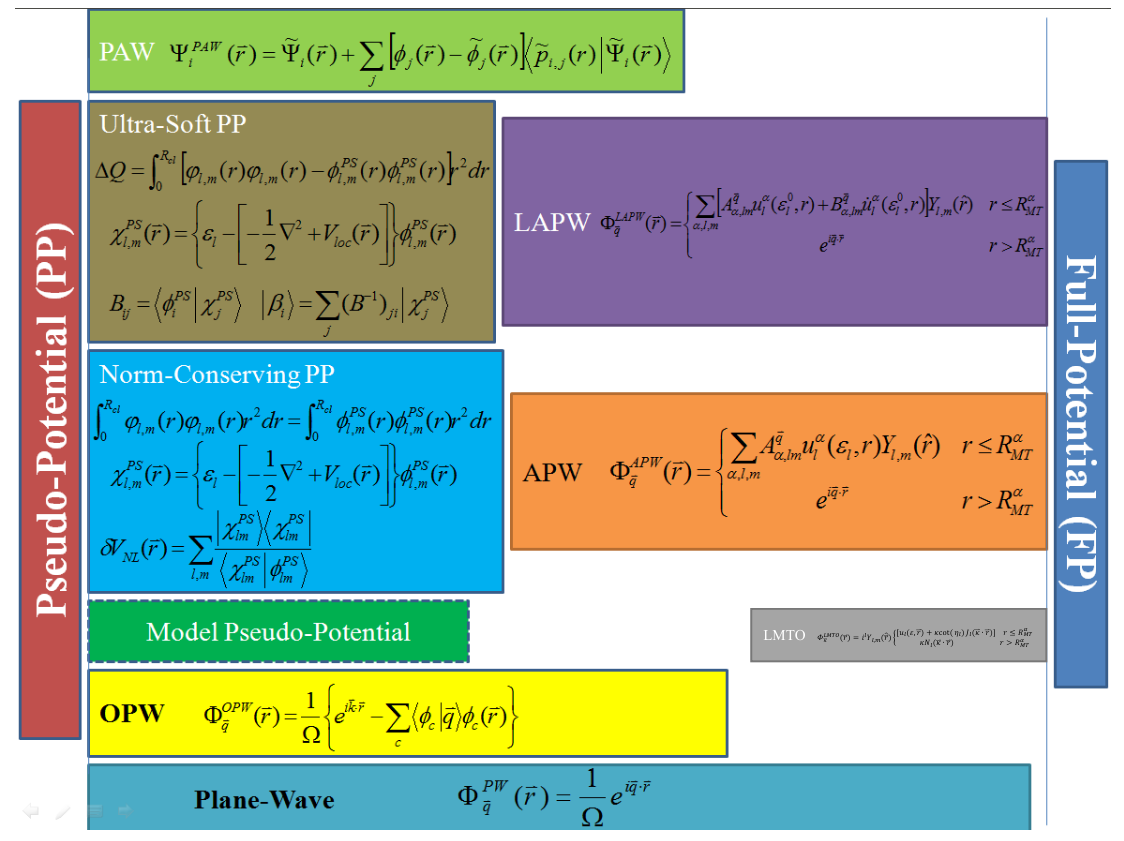
\includegraphics[height=2.80in,width=4.10in,viewport=0 0 1150 850,clip]{Figures/Pseudo-Full_Potential-2.png}
%\caption{\tiny \textrm{Pseudopotential for metallic sodium, based on the empty core model and screened by the Thomas-Fermi dielectric function.}}%(与文献\cite{EPJB33-47_2003}图1对比)
\label{Pseudo-Full_Poential}
\end{figure}
}

\subsection{赝势理论}       %Bookmark
%\section{Induction on DFT and solid-state physics}       %Bookmark
\frame
{
%\frametitle{The methods on band structure calculation}
	\frametitle{由\textrm{OPW~}到赝势}
%\vskip 10pt
%\textrm{The mainly difference of all these methods below: the basis sets and the construction of the potential}
\begin{itemize}
%\setlength{\itemsep}{5pt}
	\item 完全平面波基组\\{\fontsize{7.5pt}{5.5pt}\selectfont{少数平面波就可以很好地描述波函数在原子间的行为,近核波函数则需要大量平面波展开}}%。因此完全平面波基组虽然方便,但求体系本征态对角化的矩阵非常巨大,计算变得异常耗时。
	\item 正交平面波(\textrm{Orthogonalized plane wave, OPW})方法\\{\fontsize{7.5pt}{5.5pt}\selectfont{价电子用与芯层波函数正交的平面波展开
		\begin{displaymath}
			\phi_{\textrm{OPW}}^{\vec k+\vec G}(\vec r)=\phi_{\textrm{PW}}^{\vec k+\vec G}(\vec r)-\sum_c\langle\varphi_c|\phi_{\textrm{PW}}^{\vec k+\vec G}\rangle\varphi_c(\vec r)
		\end{displaymath}}}
	{\fontsize{7.5pt}{5.5pt}\selectfont{构造赝波函数
		\begin{displaymath}
			\tilde{\phi}_v(\vec r)=\phi_v(\vec r)+\sum_c\langle\varphi_c|\tilde{\phi}_v\rangle\varphi_c(\vec r)
		\end{displaymath}
	代入\textrm{Schr\"odinger}方程
		$$\hat H|\tilde{\phi}_v\rangle-\sum_c\langle\varphi_c|\tilde{\phi}_v\rangle\hat H|\varphi_c\rangle=\varepsilon_v|\tilde{\phi}_v\rangle-\varepsilon_v\sum_c\langle\varphi_c|\tilde{\phi}_v\rangle|\varphi_c\rangle$$
		可有$$\hat H|\tilde{\phi}_v\rangle+\textcolor{blue}{V^R}|\tilde{\phi}_v\rangle=\textcolor{blue}{\varepsilon_v}|\tilde{\phi}_v\rangle$$
		这里排斥势是$$V^R(\vec r,\vec r^{\prime})=\sum_c(\varepsilon_v-\varepsilon_c)|\varphi_c(\vec r^{\prime})\rangle\langle\varphi_c(\vec r)|$$}}
\end{itemize}
}

\frame
{
	\frametitle{由\textrm{OPW~}到赝势}
	\textrm{Phillips-Kleinman}指出,赝势($V^{e\!f\!f}$)-赝波函数(可用$\phi_{PW}^{\vec k+\vec G}$展开)满足\textrm{Schr\"odinger}方程%\upcite{PR116-287_1959}
	$$\bigg(-\dfrac12\nabla^2+\textcolor{red}{V^{e\!f\!f}}\bigg)|\tilde{\phi}_v\rangle=\textcolor{blue}{\varepsilon_v}|\tilde{\phi}_v\rangle$$
	其中$\textcolor{red}{V^{e\!f\!f}}=V(\vec r)+\textcolor{blue}{V^R}$
	\begin{itemize}
		\item 赝势-赝波函数的本征值$\varepsilon_v$与真实体系的价电子能量本征值等价
		\item 赝势$\textcolor{red}{V^{e\!f\!f}}$比$V(\vec r)$平滑得多,并且$\textcolor{blue}{V^R}$是非局域的排斥势
			\begin{displaymath}
				\begin{aligned}
					\textcolor{blue}{V^R}f(\vec r)=&\sum_c(\varepsilon_v-\varepsilon_c)\varphi_c(\vec r)\int\varphi_c^{\ast}(\vec r^{\prime})f(\vec r^{\prime})\mathrm{d}\vec r^{\prime} \\
					=&\int V^R(\vec r,\vec r^{\prime})f(\vec r^{\prime})\mathrm{d}\vec r^{\prime}
				\end{aligned}
			\end{displaymath}
%			这里$$V^R(\vec r,\vec r^{\prime})=\sum_c(\varepsilon_v-\varepsilon_c)|\varphi_c(\vec r^{\prime})\rangle\langle\varphi_c(\vec r)|$$
	\end{itemize}
}

\frame
{
\frametitle{赝势的评估}
赝势(\textrm{Pseudo Potential, PP})方法是在正交平面波的基础上发展起来的,构造出平缓的势函数代替核的强吸引作用和芯层电子的排斥作用,用平缓的函数取代波函数近核时的震荡。
\begin{itemize}
\setlength{\itemsep}{5pt}
	\item 赝势-平面波方法,只需要少量平面波可展开赝波函数,大大提升了计算效率;但是赝波函数不能很好地反映与电子近核行为有关的性质。
	\item 赝势的构造并不唯一,考核构造赝势的两大指标:~\\“柔软程度”\textrm{(Soft)}与“可移植性”\textrm{(transferability)}
\end{itemize}
\begin{figure}[h!]
\centering
\vspace*{-0.10in}
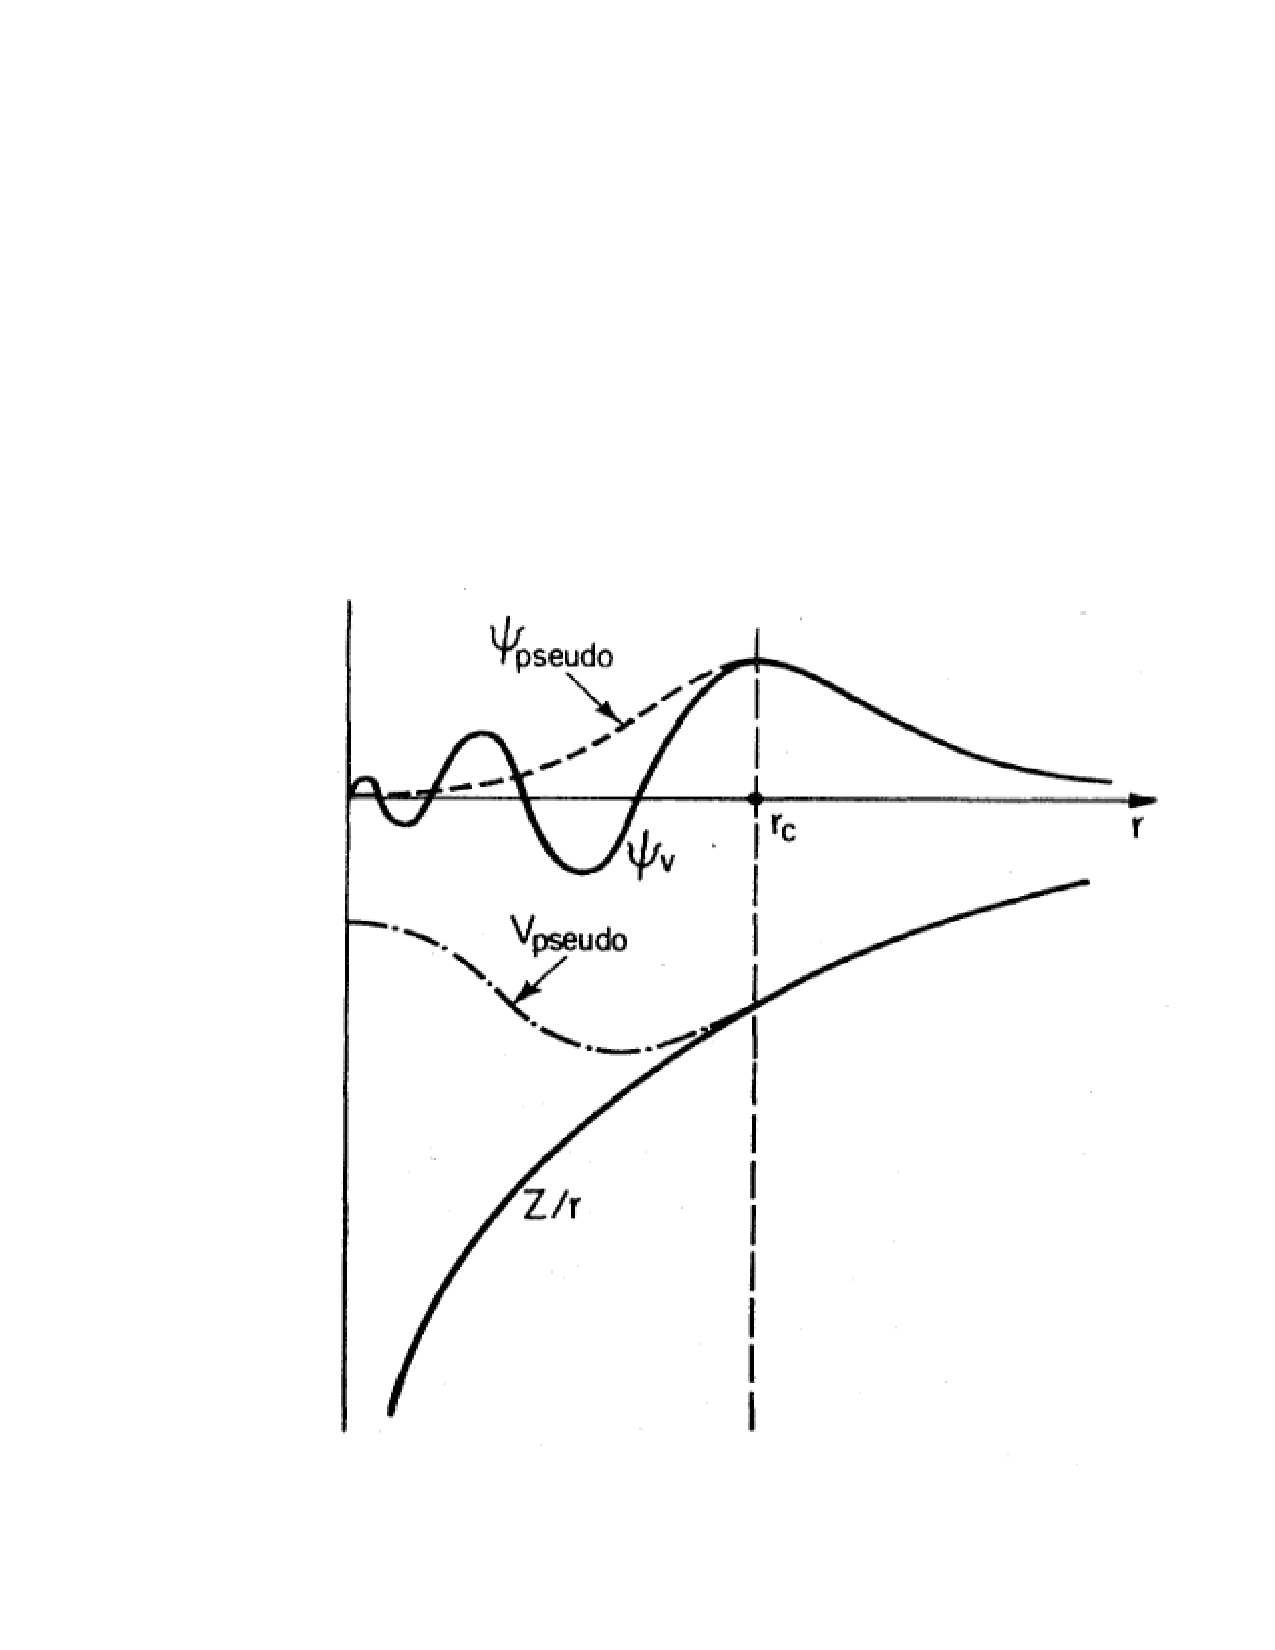
\includegraphics[height=1.35in,width=1.40in,viewport=154 100 562 508,clip]{Figures/Pseudo.pdf}
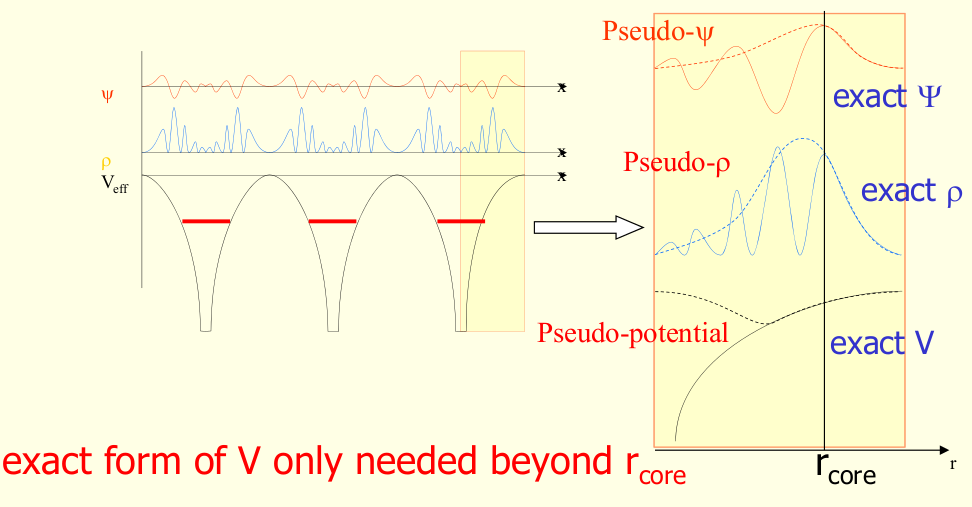
\includegraphics[height=1.35in,width=2.55in,viewport=1 1 980 500,clip]{Figures/Pseudo-2.png}
\caption{\tiny \textrm{The Pseudo wave function and Pseudo potential.}}%(与文献\cite{EPJB33-47_2003}图1对比)
\label{Pseudo_Potential-Wave}
\end{figure}
}

\frame
{
	\frametitle{第一原理赝势}
		由第一原理求解出全电子波函数(径向部分)$P_{n,l}(r)$
			\begin{displaymath}
				\bigg[-\dfrac12\dfrac{\mathrm{d}^2}{\mathrm{d}r^2}+\dfrac{l(l+1)}{2r^2}+V(\rho,r)\bigg]P_{n,l}(r)=\varepsilon_{n,l}P_{n,l}(r)
			\end{displaymath}
			这里$V(\rho,r)$是自洽单电子势
			$$V(\rho,r)=-\frac{Z}r+V_{\mathrm H}(\rho,r)+V_{XC}^{\mathrm{LDA}}(\rho(r))$$
			$V_{\mathrm H}(\rho,r)$是\textrm{Hartree}势,$V_{XC}^{\mathrm{LDA}}(\rho(r))$是交换-相关势

			由此构造赝波函数$P_l^{\mathrm{PP}}(r)$,满足
			$$P_l^{\mathrm{PP}}(r)=P_l^{\mathrm{AE}}(r),\quad r>r_{l}^c$$
			进而构造赝势$V_{\mathrm{src},l}^{\mathrm{PP}}(r)$
			$$V_{\mathrm{src},l}^{\mathrm{PP}}(r)=\varepsilon_l-\dfrac{l(l+2)}{2r^2}+\dfrac{1}{2P_l^{\mathrm{PP}}(r)}\dfrac{\mathrm{d}^2}{\mathrm{d}r^2}P_l^{\mathrm{PP}}(r),\quad r<r_{l}^c$$
}

\frame
{
	\frametitle{模守恒\textrm{(Norm-conserving)}条件}
%	构造赝势确定参数的边界(构造条件)
	\begin{enumerate}
		\item 价电子赝波函数的能量本征值与对应全电子波函数能量本征值相等:~$\varepsilon_l^{\mathrm{PP}}=\varepsilon_l^{\mathrm{AE}}$
		\item 价电子赝波函数与真实电子波函数的径向部分在截断半径$r_{c,l}$外相同:~$\psi_l^{\mathrm{PP}}(r)=\psi_l^{\mathrm{AE}}(r),\quad r>r_{l}^c$
		\item 价电子赝波函数与真实电子波函数的对数导数在截断半径$r_{c,l}$处相等:~$D_l^{\mathrm{PP}}(r)=D_l^{\mathrm{AE}}(r),\quad r\geqslant r_{l}^c$\\
		这里$D_l(\varepsilon,r)=r\frac{\psi_l^{\prime}(\varepsilon,r)}{\psi_l(\varepsilon,r)}=r\dfrac{\mathrm{d}}{\mathrm{d}r}\ln\psi_l(\varepsilon,r)$
		\item 价电子赝波函数与真实电子波函数在截断半径$r_{l}^c$内的积分电荷相等(\textcolor{red}{模守恒条件})
			$$Q_l=\int_0^{r_{l}^c}\mathrm{d}rr^2|\psi_l^{\mathrm{PP}}(r)|^2=\int_0^{r_{l}^c}\mathrm{d}rr^2|\psi_l^{\mathrm{AE}}(r)|^2$$
		\item 价电子赝波函数与真实电子波函数的对数导数一阶能量导数$\mathrm{d}D_l(\varepsilon,r)/\mathrm{d}\varepsilon$在截断半径$r_{l}^c$处及以外相等
	\end{enumerate}
}

\frame
{
	\frametitle{模守恒\textrm{(Norm-conserving)}条件}
\begin{figure}[h!]
\centering
\vspace*{-0.10in}
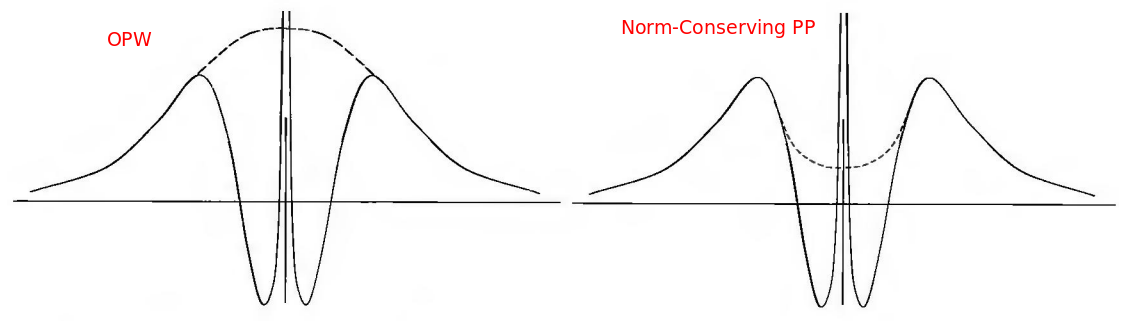
\includegraphics[height=1.30in,width=4.17in,viewport=0 0 1150 350,clip]{Figures/Pseudo-OPW_NCPP.png}
\caption{\tiny \textrm{Schematic example of a valence function that has the character of a $3s$ orbital near the nucleus and two examples of smooth functions (dashed lines) that equal the full wave-function outside the core region. Left: the smooth part of the valence function defined by OPW-like equation; Right: a smooth pseudo-function that satisfies the norm-conservation condition.}}%(与文献\cite{EPJB33-47_2003}图1对比)
\label{Pseudo-OPW_NCPP}
\end{figure}
}

\frame
{
	\frametitle{赝势去屏蔽}
	第一原理赝势建立了赝波函数与对应赝势的一一对应关系,但该赝势包含了电子屏蔽(原子、离子环境)信息,去屏蔽后的赝势对环境依赖更低,“可移植性”更好
	$$V_{\mathrm{ion},l}^{\mathrm{PP}}(r)=V_{\mathrm{src},l}^{\mathrm{PP}}(r)-V_{\mathrm{H},l}^{\mathrm{PP}}(r)-V_{XC,l}^{\mathrm{PP}}(r)$$
	去屏蔽过程中,特别需要注意$V_{XC,l}^{\mathrm{PP}}(r)$的处理
	$$V_{XC,l}^{\mathrm{PP}}(r)=V_{XC}^{\mathrm{PP}}([n_l^{\mathrm{PP}}],r)+\big[V_{XC}^{\mathrm{PP}}([n_l^{\mathrm{PP}}+n^{core}],r)-V_{XC}^{\mathrm{PP}}([n_l^{\mathrm{PP}}],r)\big]$$
}

\frame
{
\frametitle{超软赝势}
\begin{itemize}
\setlength{\itemsep}{5pt}
	\item 赝势构造的模守恒条件
%		\begin{displaymath}
%			\int_0^{r_c}\mathrm{d}\vec r\varphi^{\ast PS}(\vec r)\varphi^{PS}(\vec r)=\int_0^{r_c}\mathrm{d}\vec r\varphi^{\ast}(\vec r)\varphi(\vec r)
%		\end{displaymath}
	很好地解决了赝势可移植性问题,但对$1s$、$2p$、$3d$等轨道,模守恒方案构造的赝势过于“硬”,所需平面波基组依然非常大
	\item 超软\textrm{(Ultra-soft)}赝势,解除模守恒条件,实现对第一、第二周期元素的高效计算
\end{itemize}
\begin{figure}[h!]
\vspace*{-0.10in}
\centering
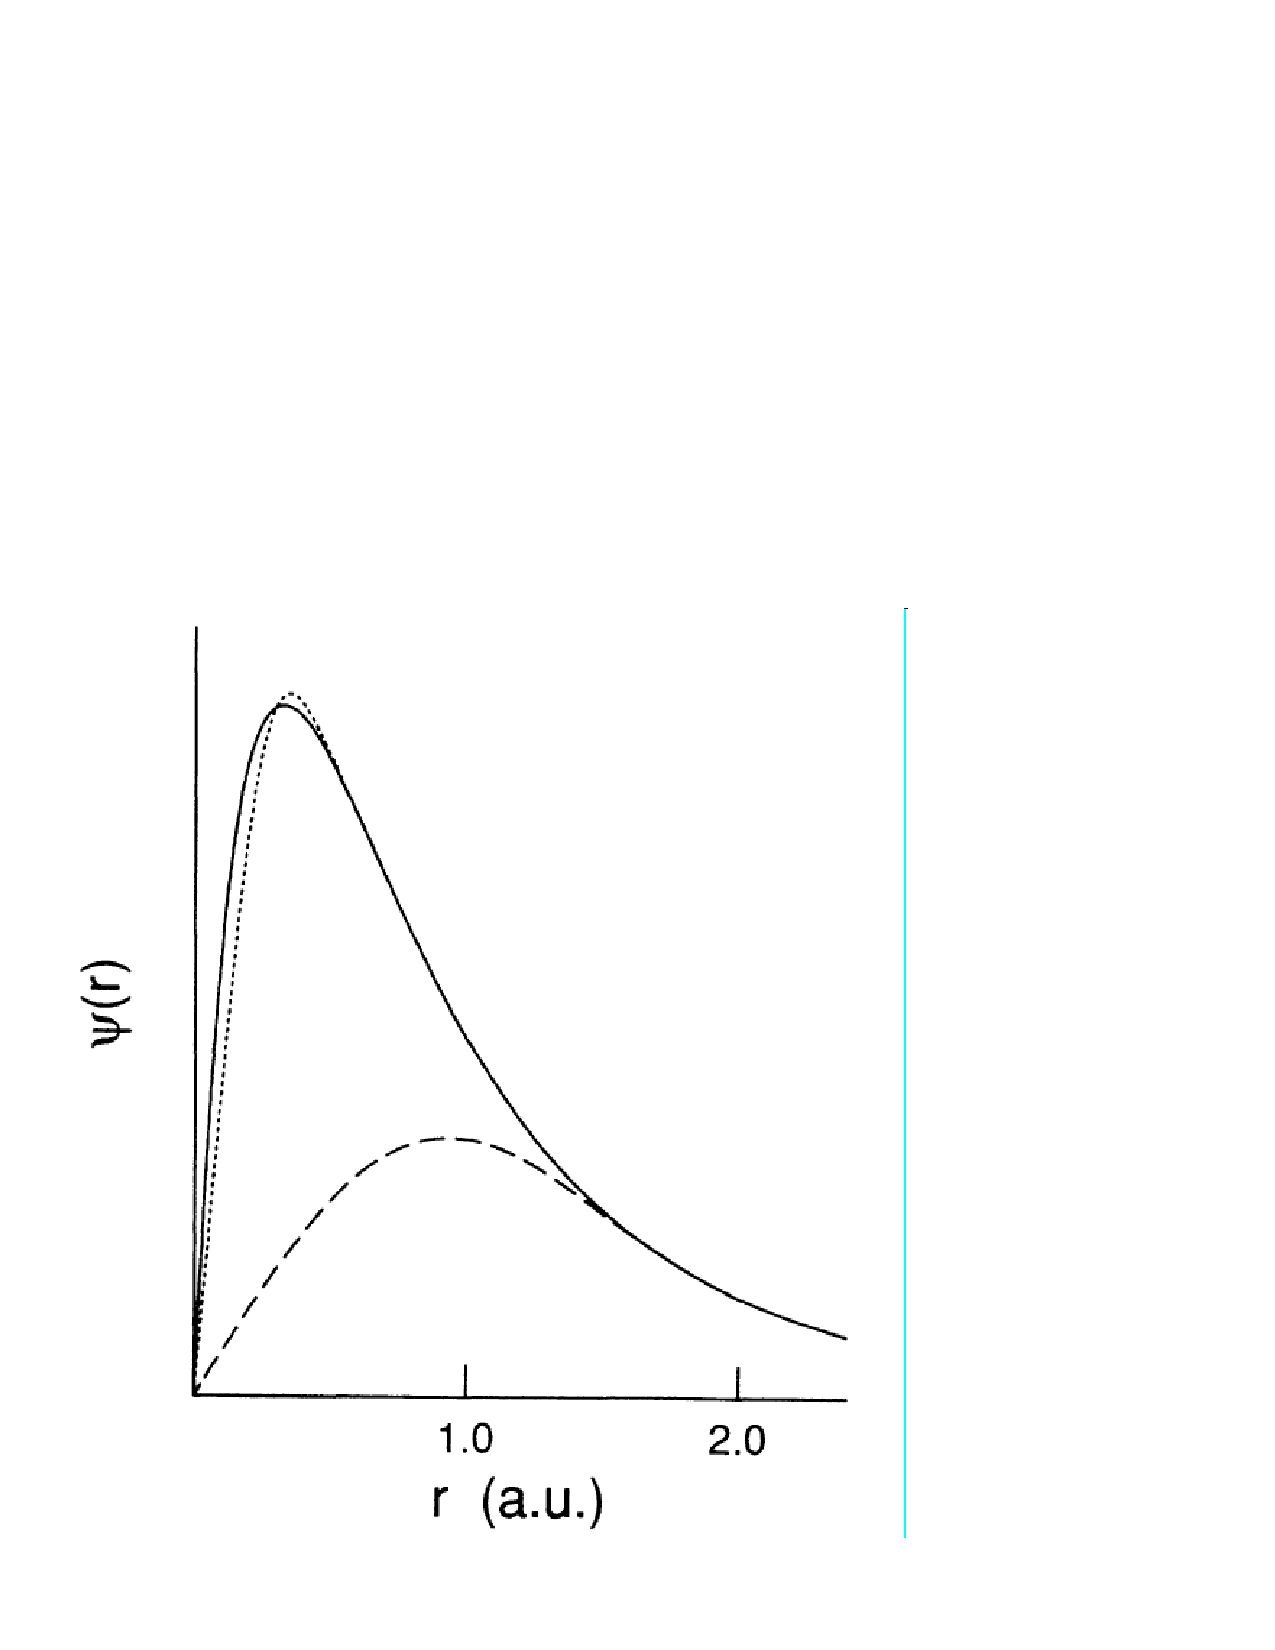
\includegraphics[height=1.35in,width=1.40in,viewport=30 55 415 500,clip]{Figures/Norm-US-wave.pdf}
\caption{\tiny \textrm{Oxygen 2} \textit{p} \textrm{radical wave function (solid), NC-pseudo-wave (dotted) and US-pseudo-wave (dashed).}}%(与文献\cite{EPJB33-47_2003}图1对比)
\label{Norm-US-wave}
\end{figure}
}

\frame
{
\frametitle{补偿电荷与多极矩}
根据电动力学定理:\\\textcolor{blue}{如果球\textrm{S}内的电荷密度分布$\rho(\vec r)$,在球外某点$\vec r$产生的势是由电荷密度的多极矩确定}:
\begin{figure}[h!]
\vspace*{-15pt}
\centering
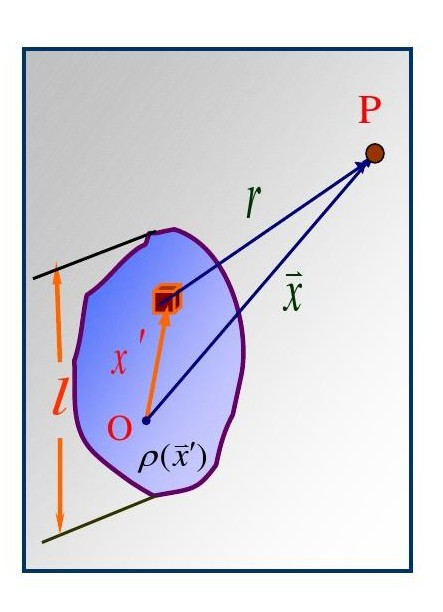
\includegraphics[height=1.25in,width=1.32in,viewport=1 22 507 575,clip]{Figures/potential_multipole.jpg}
%\caption{\tiny \textrm{From Muffin-tin Potential to Full Potential}}%(与文献\cite{EPJB33-47_2003}图1对比)
\label{Potential-multipole}
\end{figure}
\begin{displaymath}
	V(\vec r)=\sum_{l=0}^{\infty}\sum_{m=-l}^{l}\dfrac{4\pi}{2l+1}q_{lm}\dfrac{Y_{lm}(\hat{\vec r})}{r^{l+1}}
\end{displaymath}
其中多极矩$q_{lm}$由下式计算
\begin{displaymath}
	q_{lm}=\int_SY_{lm}^{\ast}(\hat{\vec r})r^l\rho(\vec r)\mathrm{d}^3r
\end{displaymath}
}

\frame
{
\frametitle{超软赝势的构造}
\textrm{Vanderbilt}建议构造赝波函数时放弃模守恒约束条件,只要求价电子赝波函数与真实电子波函数的径向部分在截断半径$r_{l}^c$外相同,由此得到的赝势显然非\textrm{Hermitian},但是通过构造\\\textcolor{blue}{\textrm{Hermitian}重叠算符}
\begin{displaymath}
	\mathbf{S}=\mathbf{1}+\sum_{i,j}Q_{ij}|\beta_j\rangle\langle\beta_i|
\end{displaymath}
以及\textcolor{blue}{\textrm{Hermitian}赝势算符}
\begin{displaymath}
	\tilde V^{\mathrm{NL}}=\sum_{i,j}\mathbf{D}_{i,j}|\beta_j\rangle\langle\beta_i|
\end{displaymath}
这里\textcolor{blue}{
\begin{displaymath}
	\mathbf{D}_{ij}=B_{ij}+\varepsilon_iQ_{ij}
\end{displaymath}}
模守恒约束下的标准本征值方程将变成广义本征值方程
\begin{displaymath}
	(T+V_{\mathrm{loc}}+\tilde V^{\mathrm{NL}}-\varepsilon\mathbf{S})|\phi\rangle=0
\end{displaymath}
}

\frame
{
\frametitle{超软赝势的特点}
\textrm{Vanderbilt}的超软赝势构造方案最大的优点是
\begin{itemize}
	\item \textcolor{purple}{解除模守恒约束}:~有助于增加赝波函数的截断半径,系统提高赝势的柔软程度
	\item \textcolor{purple}{引入多个参考能量$\varepsilon_l$}:~使得模守恒条件下只在特定参考能量$\varepsilon$处成立的对数导数连续条件,扩展到参考能量$\varepsilon_l$区间范围内,这大大提高了赝势的适用范围(可移植性)
\end{itemize}

相应的,超软赝势计算中,电子密度表达形式为
\begin{displaymath}
	n(r)=\sum_nf_n|\phi_n(r)|^2+\sum_{n,ij}f_n\langle\phi_n|\beta_j\rangle\langle\beta_i|\phi_n\rangle Q_{ij}(r)
\end{displaymath}
这里补偿电荷$Q_{ij}(r)$定义为
\begin{displaymath}
	Q_{ij}(r)=\phi_i^{\mathrm{AE}}(r)\phi_j^{\mathrm{AE}}(r)^{\ast}-\phi_i^{\mathrm{US}}(r)\phi_j^{\mathrm{US}}(r)^{\ast}
\end{displaymath}
}

\subsection{\rm{APW~}与\rm{LAPW~}方法}
\frame
{
\frametitle{\textrm{APW}方法}
\begin{figure}[h!]
\centering
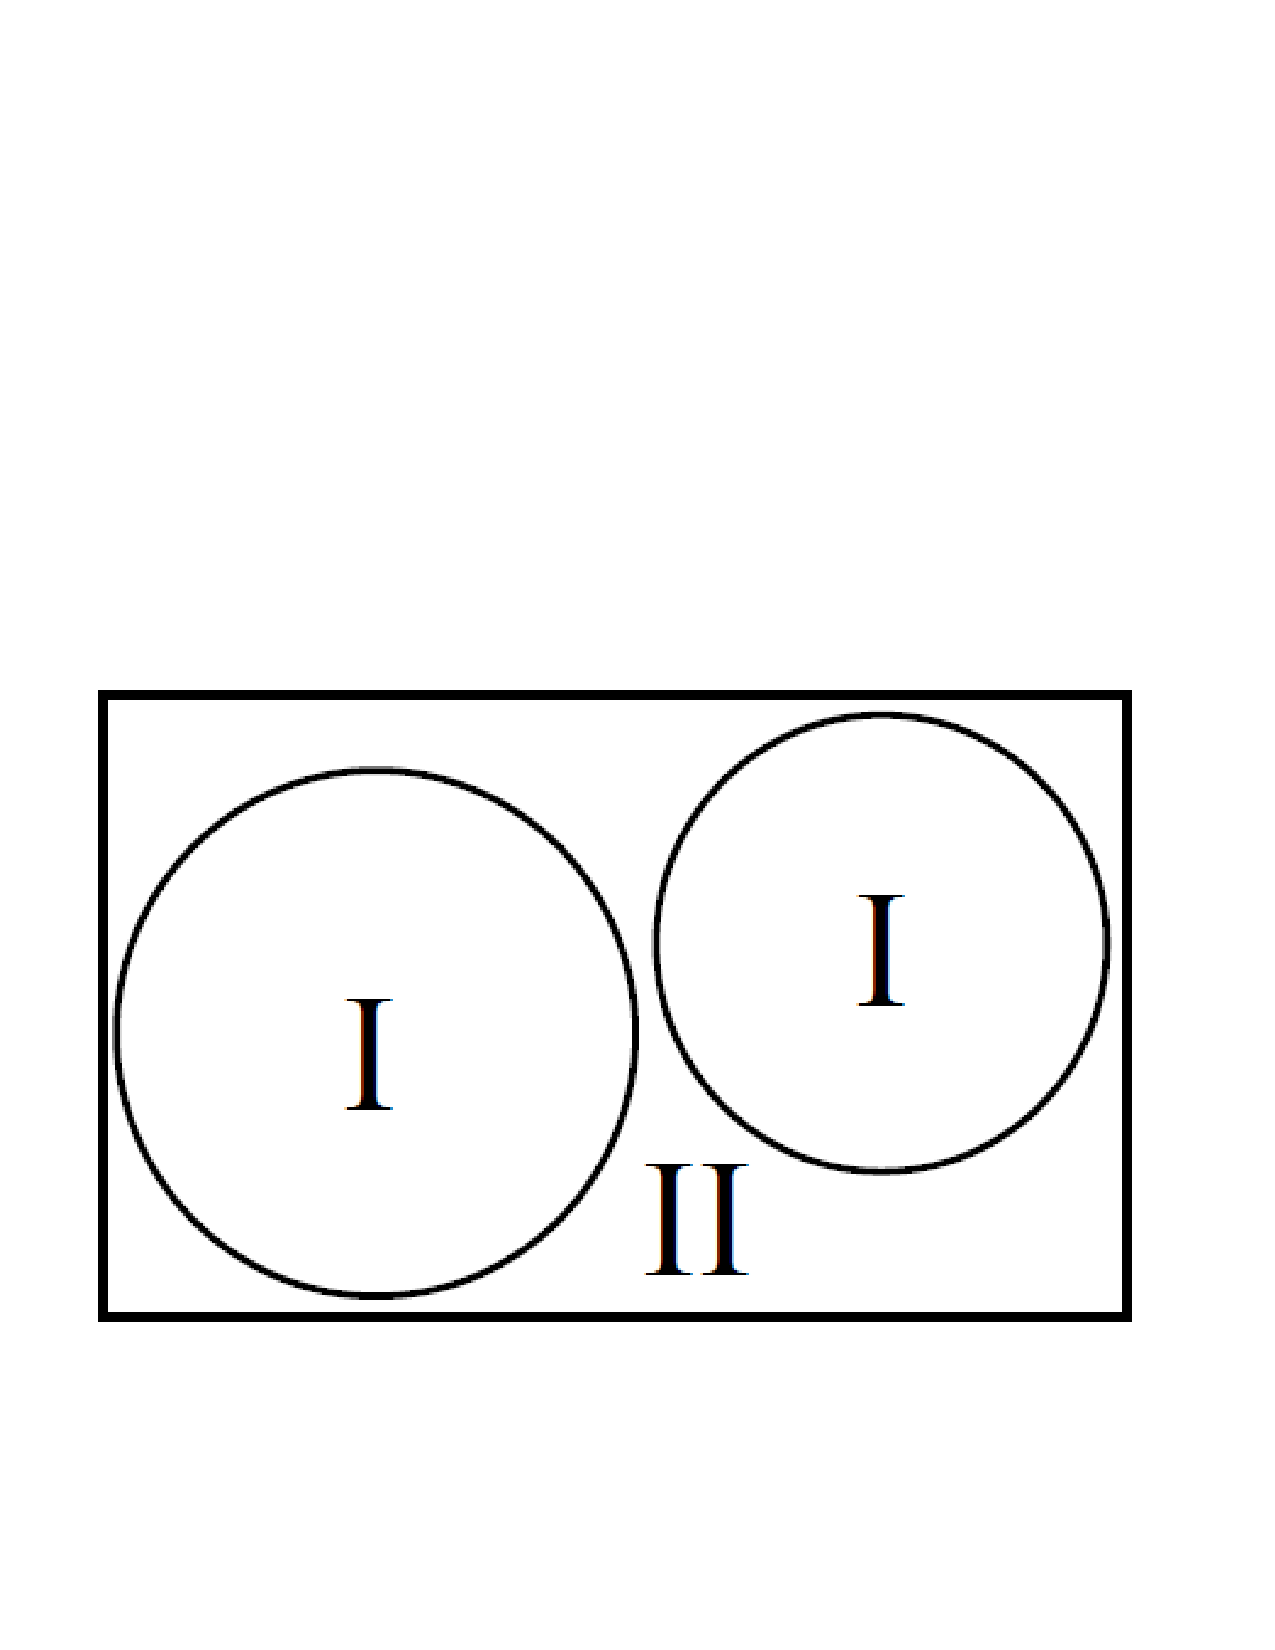
\includegraphics[height=1.10in,width=1.80in,viewport=40 150 545 465,clip]{Figures/Muffin_tin.pdf}
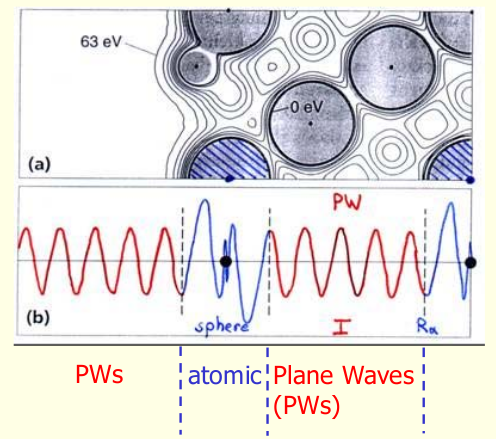
\includegraphics[height=1.10in,width=1.45in,viewport=1 20 485 435,clip]{Figures/APW.png}
\caption{\tiny \textrm{Partitioning of the unit cell into atomic spheres(I) and an interstitial region(II)}}%(与文献\cite{EPJB33-47_2003}图1对比)
\label{Muffin_tin-2}
\end{figure}
\begin{displaymath}
\hskip -28pt\footnotesize \varphi(\vec k_j,\vec r)=\left\{
  \begin{aligned}
    &\Omega^{-1/2}\exp[i\vec k_j\cdot\vec r],&|\vec r-\vec r_s|>R_{\mathrm{MT}}^s\\
    &\sum_{lm}A_{lm}^{\vec k_j}u_l(|\vec r-\vec r_s|,E)Y_{lm}(\widehat{\vec r-\vec r_s}),&|\vec r-\vec r_s|\leqslant R_{\mathrm{MT}}^s
  \end{aligned}
\right.
\end{displaymath}
}

\frame
{
	\frametitle{空间两部分函数在球面上的衔接}
	\textrm{Huygens}原理:~\textcolor{blue}{平面波可以在各个原子球中心用球谐函数展开}:
	\begin{displaymath}
		\mathrm{e}^{\mathrm{i}\vec k\cdot\vec r}=4\pi\sum_{l=0}^{\infty}\sum_{m=-l}^l\mathrm{i}^lj_l(|\vec k|r)Y_{lm}^{\ast}(\hat{\vec k})Y_{lm}(\hat{\vec r})
	\end{displaymath}
	其中$j_l(|\vec k|r)$是$l$-阶球\textrm{Bessel}函数,$\hat{\vec k}$和$\hat{\vec r}$分别是矢量$\vec k$和$\vec r$与直角坐标$z$-轴的夹角$\theta$和$\varphi$

	要求空间中不同区域函数在球面上连续,可调参数$A_{lm}^{\vec k}$可为下式确定
\begin{displaymath}
	A_{lm}^{\vec k}=4\pi\mathrm{e}^{\mathrm{i}\vec k\cdot\vec r_s}\mathrm{i}^lY_{lm}^{\ast}(\hat{\vec k})j_l(|\vec k|R_{MT}^s)/u_l(R_{MT}^s,E)
\end{displaymath}
\textrm{APW}的问题:\textcolor{blue}{球面参数$A_{lm}^{\vec k}$对能量$E$依赖,由此构造的久期方程\footnote{\fontsize{7.2pt}{6.2pt}\selectfont{久期方程\textrm{secular~equation},\textrm{secular}来自拉丁语\textrm{saeculum},本意为一代人、一个时期、一个时代、一个世界等意思。其名词在拉丁语中就作为世纪讲。汉译\textrm{secular}为久期,是取\textrm{long-term}的意思(实为慢,\textrm{slow~in~comparison~to~the~annual~motion}的意思),与期待\textrm{(expectation)}无关。}}非线性的}
}

\frame
{
\frametitle{\textrm{LAPW}方法}
%\small\textrm{APW}方法的困难,久期方程不能化成广义本征值方程的形式(久期方程对能量$E$是非线性的)为了克服这一困难,人们提出线性化方法,
\textrm{O.~K.~Andersen~}提出\textrm{LAPW}方法\upcite{Singh}:将$u_l(r,E)$在某一合适的$E_l$值附近对$E$的一阶微商{$\left.\dfrac{\textrm{d}u_l(r,E)}{\textrm{d}E}\right|_{E_l}\equiv\dot u_l(r,E_l)$}\\代入\textrm{APW}基函数中可得\textrm{LAPW}方法的基函数:
{\fontsize{7.5pt}{3.3pt}\selectfont
$$\hskip -14pt \varphi(\vec k_j,\vec r)=\left\{
  \begin{aligned}
    &\Omega^{-1/2}\exp[i\vec k_j\cdot\vec r],&|\vec r-\vec r_s|>R_{\mathrm{MT}}^s\\
    &\sum_{lm}[A^{\vec k_j}_{lm}u_l(|\vec r-\vec r_s|,E_l)+B^{\vec k_j}_{lm}\dot u_l(|\vec r-\vec r_s|,E_l)]Y_{lm}(\widehat{\vec r-\vec r_s}),&|\vec r-\vec r_s|\leqslant R_{\mathrm{MT}}^s
  \end{aligned}
\right.$$
%$$\Psi_{\vec k}(\vec r)=\int_{\Omega}\tilde G_{\vec k}(\vec r-\vec r\,^\prime;E)V(\vec r\,^\prime)\Psi_{\vec k}(\vec r\,^\prime)\textrm{d}\vec r\,^\prime$$
根据基函数在\textrm{MT}球面上连续到一阶,确定系数$A^{\vec k}_{lm}$,$B^{\vec k}_{lm}$的值。}
\begin{figure}[h!]
	\vskip -3pt
\centering
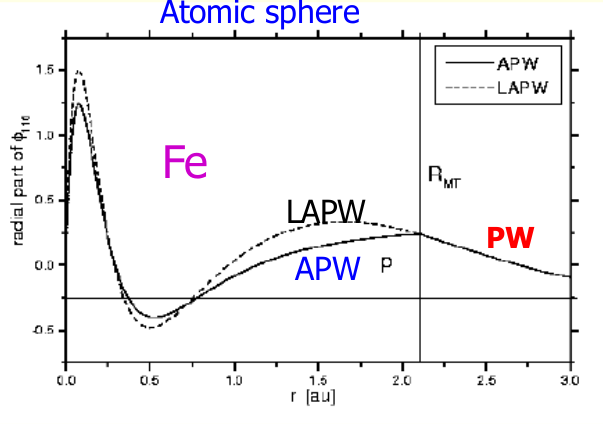
\includegraphics[height=1.10in,width=1.88in,viewport=1 20 585 435,clip]{Figures/WIEN2k-LAPW.png}
\caption{\tiny \textrm{Partitioning of the unit cell into atomic spheres(I) and an interstitial region(II)}}%(与文献\cite{EPJB33-47_2003}图1对比)
\label{Muffin_tin-3}
\end{figure}
}

\subsection{\rm{MTO~}与\rm{LMTO~}方法}
\frame
{
\frametitle{\textrm{MTO}方法}
\textrm{MTO (Muffin-tin Orbial)}方法是\textrm{Andersen}于\textrm{1971}年提出的局域缀加基函数方案\upcite{Andersen_Book}
%\textrm{MTO}的
\vskip 5pt
\textcolor{blue}{目的:~用最小基组方法解析电子结构}
\begin{itemize}
	\item \textcolor{red}{物理图像}:~和\textrm{APW}方法类似,要求基函数在\textrm{MT}球内、外分区域表示,并且在球面上连续
	\item \textcolor{red}{数学形式}:~基函数是最小优化基组
\end{itemize}
\begin{figure}[h!]
	\vspace{-5pt}
\centering
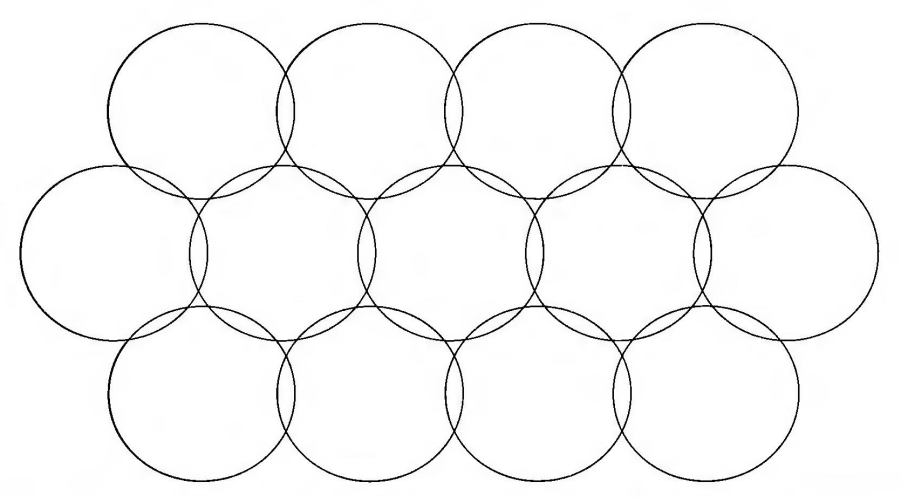
\includegraphics[height=1.20in,width=2.42in,viewport=5 0 1005 495,clip]{Figures/Atomic_sphere-appro.png}
\caption{\fontsize{6.2pt}{4.2pt}\selectfont\textrm{Atomic sphere approximation (ASA) in which the MT spheres are chosen to have the same volume as the Wigner-Seitz cell, which leads to overlapping spheres.}}
\label{Atomic_sphere-appro}
\end{figure}
}

\frame
{
	\frametitle{\textrm{MTO}方法的基函数}
\begin{figure}[h!]
	\vspace{-13pt}
\centering
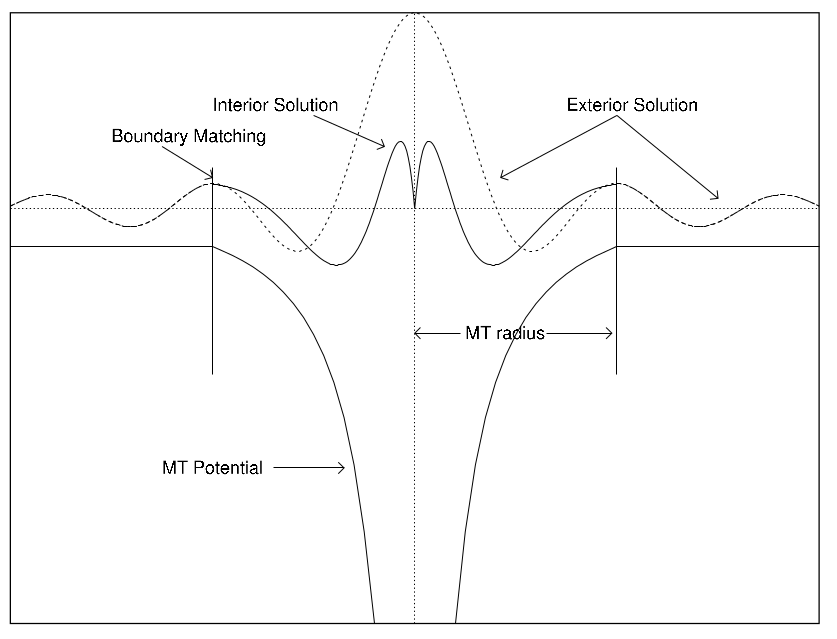
\includegraphics[height=1.25in,width=1.95in,viewport=0 0 845 635,clip]{Figures/MTO-envelope-1.png}
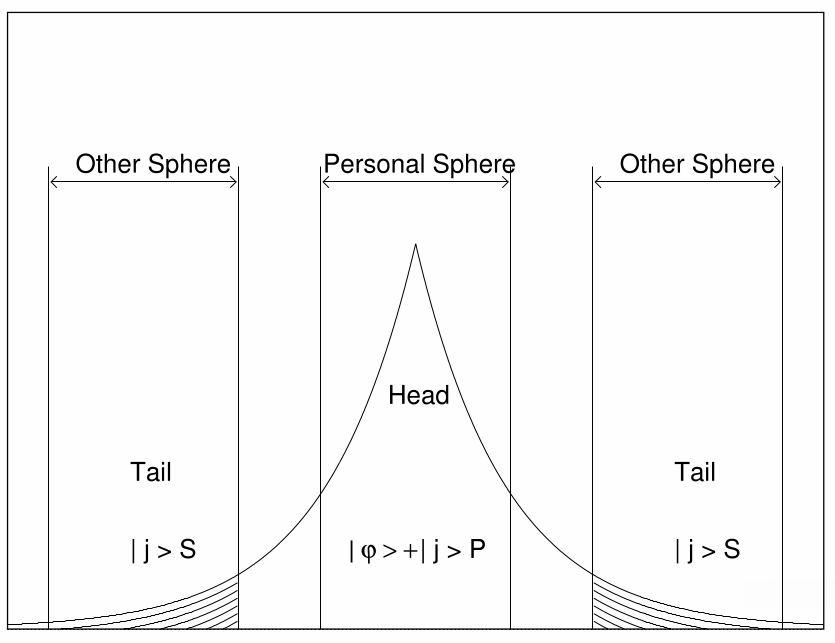
\includegraphics[height=1.25in,width=1.95in,viewport=0 0 885 635,clip]{Figures/MTO-envelope-2.png}
\caption{\tiny \textrm{The radial function of MTO expressed in different region.}}%(与文献\cite{EPJB33-47_2003}图1对比)
\label{MTO-envelope}
\end{figure}
当$q_0=0$时,构成最简单的\textrm{MTO}基函数
		\begin{displaymath}
			\hspace*{-12pt}\chi_L^{\mathrm{MTO}}(\varepsilon,0,\vec r)=\mathrm{i}^lY_L(\hat{\vec r})u_l(\varepsilon,S)\left\{
			\begin{aligned}
				&\dfrac{u_l(\varepsilon,r)}{u_l(\varepsilon,S)}-\dfrac{D_l(\varepsilon)+l+1}{2l+l}\left(\dfrac rS\right)^l&\, r\leqslant S\\
				&+\dfrac{l-D_l(\varepsilon)}{2l+1}\left(\dfrac Sr\right)^{l+1}&\, r>S
			\end{aligned}\right.
		\end{displaymath}
}

\frame
{
	\frametitle{\textrm{MTO}轨道的“尾部抵消”}
\begin{figure}[h!]
	\vspace*{-0.7in}
\centering
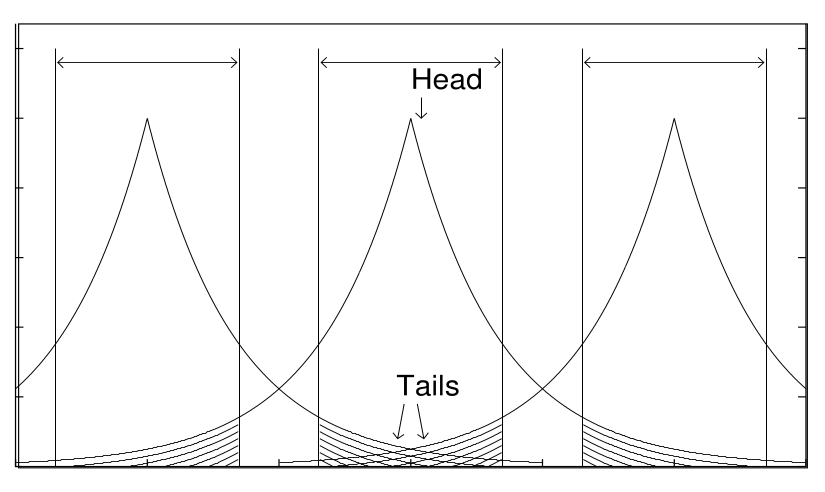
\includegraphics[height=2.55in,width=3.15in,viewport=0 0 845 635,clip]{Figures/MTO-Tail_cancellation.png}
\caption{\tiny \textrm{The wavefunction in the spere at the origin is the sum of the ``head function'' in that sphere plus the tails from neighboring spheres. The schematic illustration of the ``tail cancellation'' of the MTO.}}%(与文献\cite{EPJB33-47_2003}图1对比)
\label{MTO-tail-candellation}
\end{figure}
}

\frame
{
	\frametitle{\textrm{LMTO}方法}
	与\textrm{LAPW}方法类似,在给定能量$\varepsilon_v$和衰减常数$q_0$附近,\textrm{LMTO}的基函数球内部分用函数$\psi_l(\varepsilon_v,r)$及其对能量导数$\dot\psi(\varepsilon_v,r)$表示\\
\textcolor{blue}{\textrm{LMTO}与\textrm{MTO}基函数的区别}
	\begin{itemize}
		\item 球内部分的$\psi(\varepsilon,r)$是主要部分:~由$\psi(\varepsilon_v,r)$和$\dot\psi(\varepsilon_v,r)$线性组合
		\item 球内来自其它\textrm{MT}球的函数尾部贡献被$\dot\psi(\varepsilon_v,r)$的线性组合替代
	\end{itemize}
	由此根据物理直觉,可以把\textrm{LMTO}基函数的形式表示成
		\begin{displaymath}
			\hspace*{-12pt}\chi_L^{\mathrm{LMTO}}(\varepsilon,q_0,\vec r)=\mathrm{i}^lY_L(\hat{\vec r})\left\{
			\begin{aligned}
				&u_l(\varepsilon,r)-q_0\cot(\eta_l(\varepsilon))J_l(q_0r)&\, r\leqslant S\\
				&q_0N_l(q_0r)&\, r>S
			\end{aligned}\right.
		\end{displaymath}
		实际应用中,选定函数$J_l$和$N_l$与球\textrm{Bessel}函数$j_l$和\textrm{Neumann}函数$n_l$相似
}

\frame
{
	\frametitle{\textrm{LMTO~.vs.~LAPW}}
\begin{figure}[h!]
\centering
\vspace*{-0.15in}
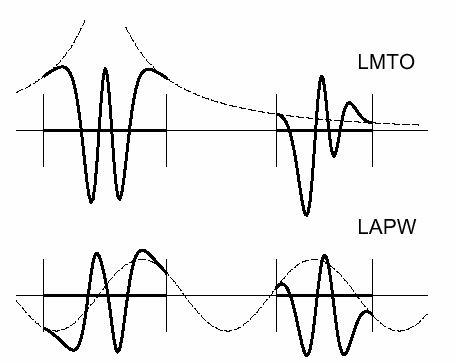
\includegraphics[height=2.50in,width=3.30in,viewport=0 0 440 350,clip]{Figures/LMTO-vs-LAPW.png}
\caption{\fontsize{5.5pt}{4.2pt}\selectfont{\textrm{Schematic illustration of LMTO vs LAPW.}}}%(与文献\cite{EPJB33-47_2003}图1对比)
\label{LMTO-vs-LAPW}
\end{figure}
}

\subsection{\rm{PAW}方法}
\frame
{
	\frametitle{\textrm{PAW}方法概要}
\begin{itemize}
	\item 与芯层态正交的全部价电子构成的\textrm{Hilbert}空间%,价电子彼此的正交使得波函数在\textrm{Muffin-tin}球内振荡
	\item 作\textcolor{red}{线性空间变换},全电子波函数$|\Psi\rangle$与赝波函数$|\tilde\Psi\rangle$满足:
		$$|\Psi\rangle=\mathbf{\tau|}\tilde\Psi\rangle$$
%	$$\tau=\mathbf{1}+\sum_{\mathrm R}\hat\tau_{\mathrm R}$$
	\item 在原子核附近的$r_c$范围内,波函数用原子分波函数展开:
	$$|\Psi\rangle=|\tilde\Psi\rangle+\sum_i(|\phi_i\rangle-|\tilde\phi_i\rangle)\langle\tilde p_i|\tilde\Psi\rangle$$
	\item 在$r_c$外$|\tilde\Psi\rangle$与$|\Psi\rangle$变换前后保持不变,因此线性变换$\mathbf{\tau}$可表示为:
	$$\mathbf{\tau}=\mathbf{1}+\sum_i(|\phi_i\rangle-|\tilde\phi_i\rangle)\langle\tilde p_i|$$
\end{itemize}
其中$|\tilde p_i\rangle$是\textrm{MT}球内的投影函数\\
$i$表示原子位置$\vec R$、原子轨道($l,m$)和能级$\epsilon_k$的指标。
}

\frame
{
%	\frametitle{\textrm{PAW}原子数据集}
	\frametitle{\textrm{PAW}方法的基本思想}
\begin{figure}[h!]
\centering
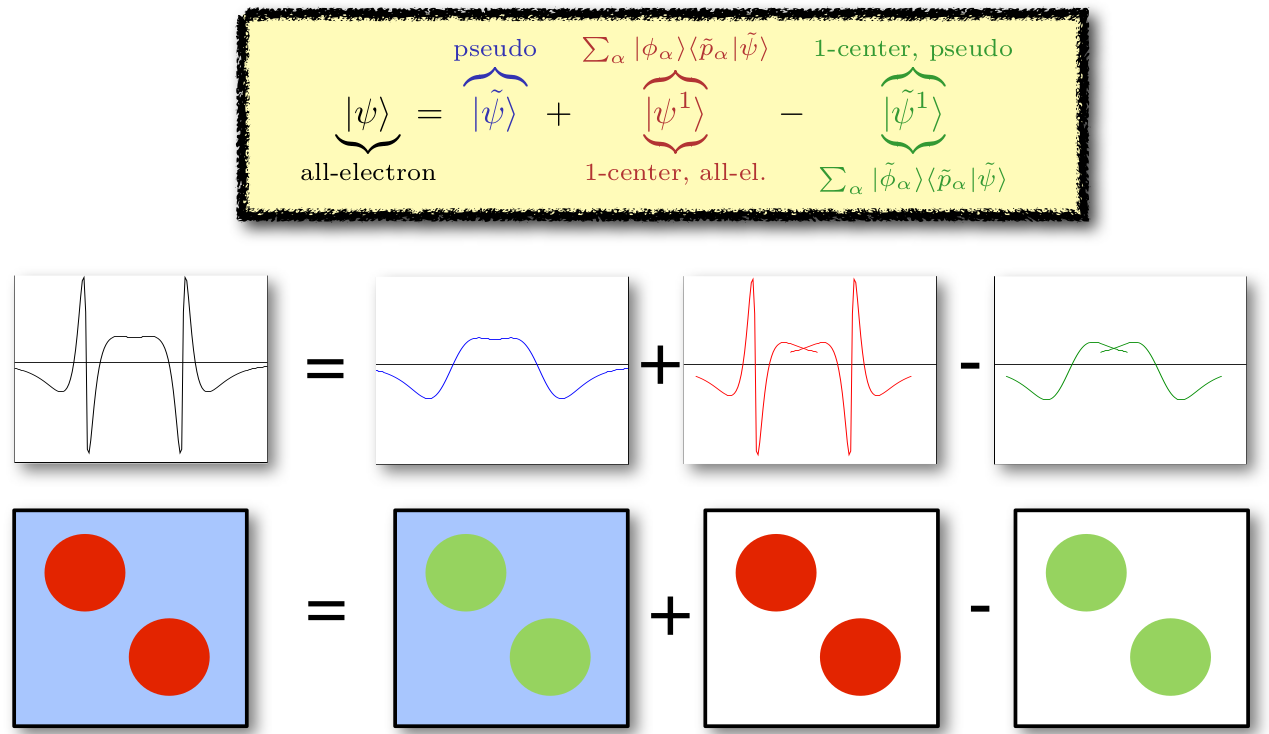
\includegraphics[height=2.3in,width=4.0in,viewport=0 0 1280 745,clip]{Figures/PAW-baseset.png}
\caption{\tiny \textrm{The Augmentation of PAW.}}%(与文献\cite{EPJB33-47_2003}图1对比)
\label{PAW_baseset}
\end{figure}
}

\frame
{
\frametitle{\textrm{PAW}方法的基本思想}
	在赝波函数$|\tilde\Psi\rangle$表象下,算符期望值计算满足$$\langle A \rangle=\langle\Psi|\mathbf{A}|\Psi\rangle=\langle\tilde\Psi|\mathbf{\tau}^{\dag}\mathbf{A}\mathbf{\tau}|\tilde\Psi\rangle=\langle\tilde\Psi|\tilde{\mathrm{A}}|\tilde\Psi\rangle$$
\begin{itemize}
	\item 一般赝算符$\tilde A$表示为
		$$\tilde A=\mathbf{A}+\sum_i|\tilde p_i\rangle(\langle\phi_i|\mathbf{A}|\phi_i\rangle-\langle\tilde\phi_i|\mathbf{A}|\tilde\phi_i\rangle)\langle\tilde p_i|$$
	\item 赝重叠算符$\tilde O$表示为
		$$\tilde O=\mathbf{1}+\sum_i|\tilde p_i\rangle(\langle\phi_i|\phi_i\rangle-\langle\tilde\phi_i|\tilde\phi_i\rangle)\langle\tilde p_i|$$
\end{itemize}
}

\frame
{
\frametitle{\textrm{PAW}方法密度计算}
在\textrm{PAW}框架下,将密度算符$|\vec r\rangle\langle\vec r|$代入,可知密度表达式为
$$n(\vec r)=\tilde n(\vec r)+n^1(\vec r)-\tilde n^1(\vec r)$$
这里
$$\tilde n(\vec r)=\sum_nf_n\langle\tilde\Psi_n|\vec r\rangle\langle\vec r|\tilde\Psi_n\rangle$$ 
$$n^1(\vec r)=\sum_{n,(i,j)}f_n\langle\tilde\Psi_n|\tilde p_i\rangle\langle\phi_i|\vec r\rangle\langle\vec r|\phi_j\rangle\langle\tilde p_j|\tilde\Psi_n\rangle$$
$$\tilde n^1(\vec r)=\sum_{n,(i,j)}f_n\langle\tilde\Psi_n|\tilde p_i\rangle\langle\tilde\phi_i|\vec r\rangle\langle\vec r|\tilde\phi_j\rangle\langle\tilde p_j|\tilde\Psi_n\rangle$$
}

%\frame
%{
%	\frametitle{\textrm{PAW Augmentation}}
%\begin{figure}[h!]
%\centering
%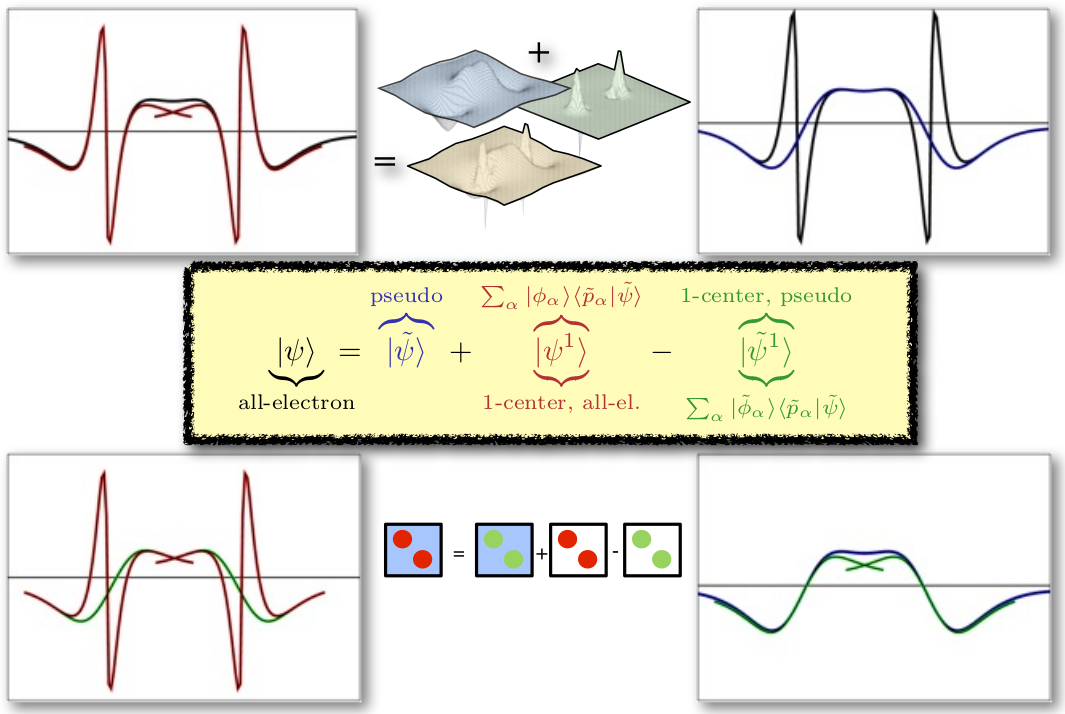
\includegraphics[height=2.3in,width=4.0in,viewport=0 0 1100 745,clip]{Figures/PAW-projector.png}
%\caption{\tiny \textrm{The projector of PAW.}}%(与文献\cite{EPJB33-47_2003}图1对比)
%\label{PAW_projector}
%\end{figure}
%}

\frame
{
\frametitle{电荷密度的重新分解}
\textrm{PAW}方法提出后有很长一段时间没有能够得到广泛应用,直到\textrm{G. Kresse}等将\textrm{Bl\"ochl}的原始方案中电荷密度计算方案重新组合后,明确了\textrm{PAW}方法与\textrm{USPP}方法的内在联系。
\begin{itemize}
	\item 芯层电荷与核电荷构成离子实电荷:$n_{Zc}=n_Z+n_c$
\end{itemize}
\begin{figure}[h!]
\centering
\vspace{-10.5pt}
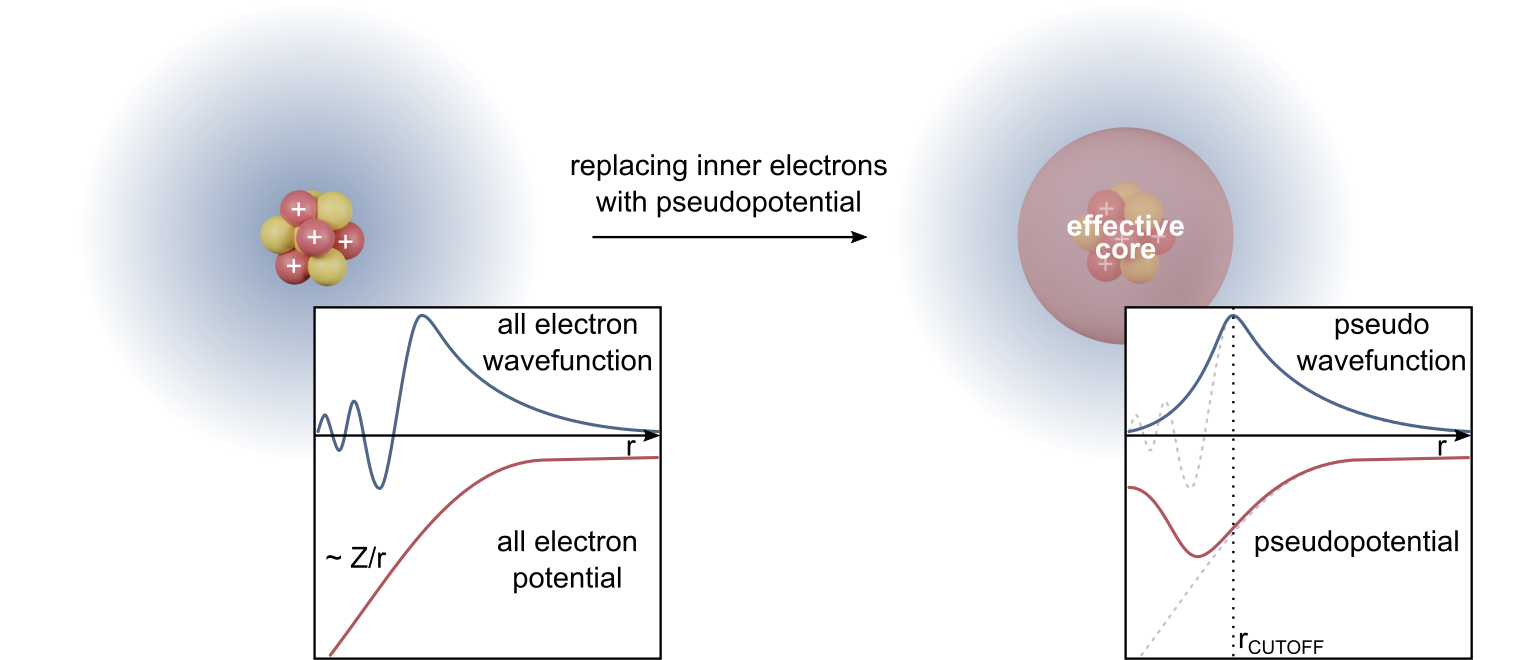
\includegraphics[height=1.5in,width=3.0in,viewport=0 0 380 190,clip]{Figures/Pseudo-potential_charge.png}
\caption{\tiny \textrm{The difference of the electron-density distributing from P.~Bl\"ochl  and from G.~Kresse.}}%(与文献\cite{EPJB33-47_2003}图1对比)
\label{PAW_Pseudo-Charge}
\end{figure}
}

		\frame[allowframebreaks]
{
\frametitle{主要参考文献}

\begin{thebibliography}{99}
{\tiny
        \bibitem{Singh}\textrm{D. J. Singh. \textit{Plane Wave, PseudoPotential and the LAPW method} (Kluwer Academic, Boston,USA, 1994)}					%
	\bibitem{PRB41-7892_1990}\textrm{D. Vanderbilt. \textit{Phys. Rev.} B, \textbf{41} (1990), 7892} 
	\bibitem{JPCM6-8245_1994}\textrm{G. Kresse and J. Hafner. J. Phys: \textit{Condens. Matter}, \textbf{6} (1994), 8245}
	\bibitem{LMTO_Book}\textrm{H. Skriver. \textit{The LMTO method} (Springer, New York, USA, 1984)}
	\bibitem{PRB50-17953_1994}\textrm{P. E. Bl\"ochl. \textit{Phys. Rev.} B, \textbf{50} (1994), 17953}
	\bibitem{PRB59-1758_1999}\textrm{G. Kresse and D. Joubert \textit{Phys. Rev.} B, \textbf{59} (1999), 1758}
	\bibitem{Andersen_Book}\textrm{O. K. Andersen. \textit{Computational Methods in Band Theory} (Plenum, New York, USA, 1971)}
	\bibitem{Nemoshkalenko-Antonov}\textrm{V. V. Nemoshkalenko and V. N. Antonov. \textit{Computational Methods in Solid State Physics} (Gordon and Breach Science Publisher, Amsterdam, The Netherlands, 1998)}
	\bibitem{Xie-Lu}谢希德、陆栋\:主编, {\textit{固体能带理论}}\:复旦大学出版社, 上海, 1998
	\bibitem{Elect_Stru}\textrm{Richard. M. Martin. \textit{Electronic Structure: Basic Theory and Practical Methods} (Cambridge University Press, Cambridge, England, 2004)}
	\bibitem{Comp_Phys}\textrm{J. M. Thijssen. \textit{Computational Physics}~\textrm{(2nd Edition)} (Cambridge University Press, Cambridge, England, 2007)}
}
\end{thebibliography}
%\nocite*{}
}

\section{计算示例:~\rm{Materials~Studio}计算}
\subsection{\rm{Materials~Studio}的安装}
\frame
{
	\frametitle{\textrm{Materials~Studio}的安装}
\begin{figure}[h!]
	\vspace{-10pt}
\centering
%\caption{\tiny \textrm{The Nolbel Prize in Chemistry 1998 Summary.}}%(与文献\cite{EPJB33-47_2003}图1对比)
\includemovie[poster, controls, mouse, url]{0.9\textwidth}{0.56\textwidth}{Figures/BIOVIA-Materials_Studio-Installation-Video-on-Windows.mp4}     %
\label{Materials-Studio_Install}
\end{figure}
}

\subsection{\rm{Materials Studio}的界面框架}
\frame
{
	\frametitle{\textrm{MS}的界面框架}
\begin{figure}[h!]
\centering
\vspace*{-0.31in}
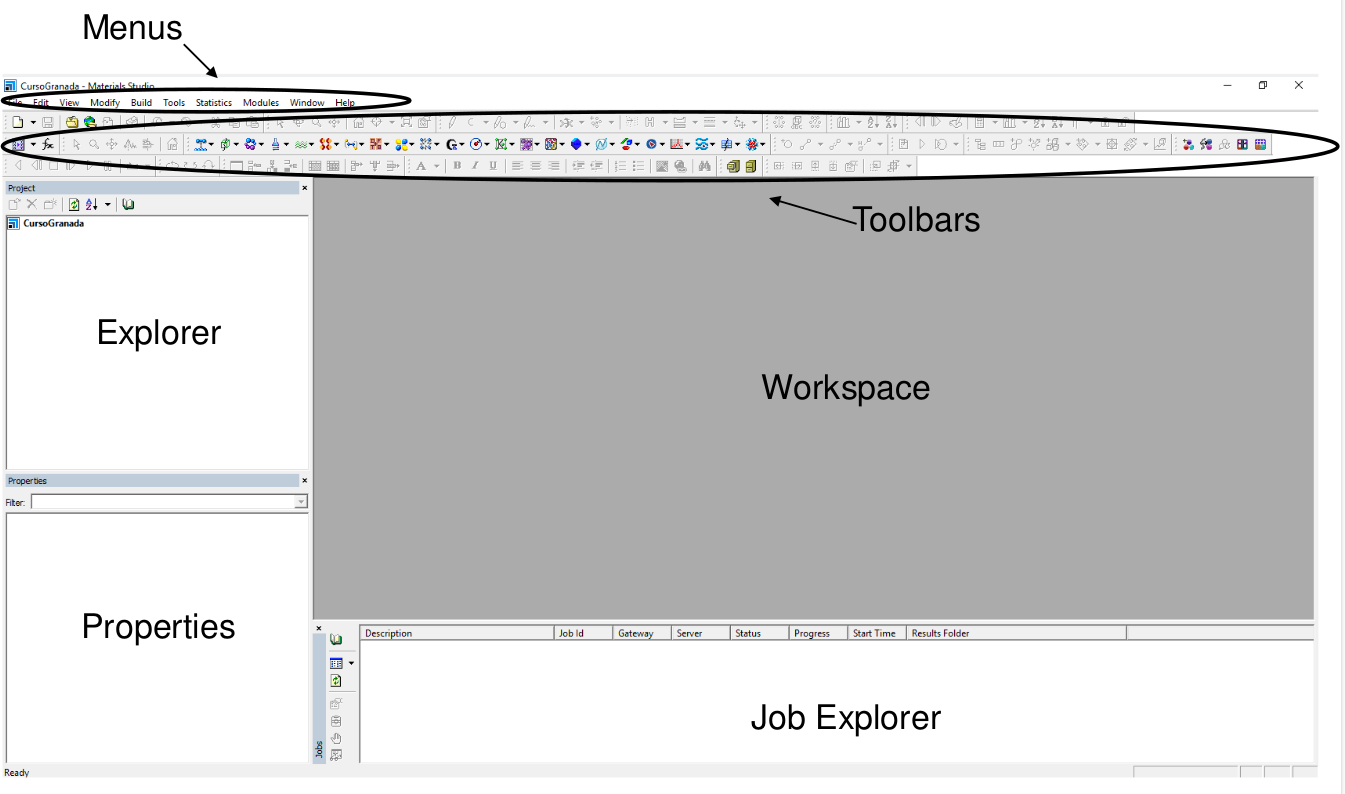
\includegraphics[height=2.45in,width=4.10in,viewport=0 0 1340 800,clip]{Figures/MS-Frame.png}
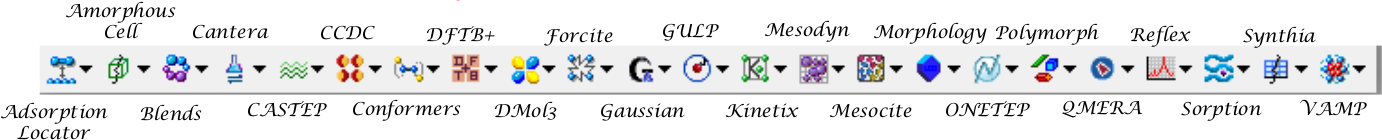
\includegraphics[height=0.45in,width=4.15in,viewport=0 0 1400 147,clip]{Figures/MS-Frame_calculators.png}
\caption{\tiny \textrm{The frame of Materials studio.}}%(与文献\cite{EPJB33-47_2003}图1对比)
\label{MS-Frame}
\end{figure}
}

\frame
{
	\frametitle{\textrm{MS}的界面框架:~\textrm{Indigo}}
\begin{figure}[h!]
\centering
\vspace*{-0.28in}
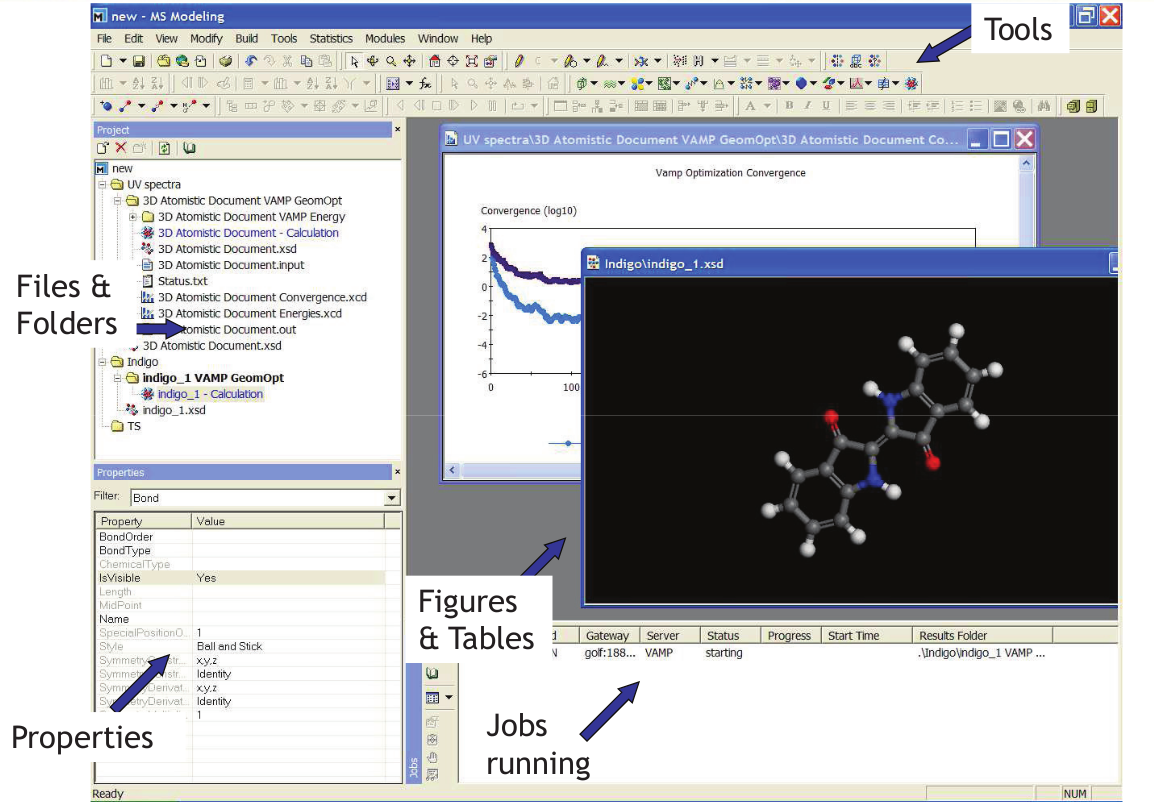
\includegraphics[height=2.85in,width=4.15in,viewport=0 0 1140 800,clip]{Figures/MS-Frame_example.png}
\caption{\tiny \textrm{The frame of Materials studio:~Example Indigo.}}%(与文献\cite{EPJB33-47_2003}图1对比)
\label{MS-Frame_example}
\end{figure}
}

\frame
{
	\frametitle{\textrm{MS:~Quick Start-01}}
\begin{figure}[h!]
\centering
\vspace*{-0.21in}
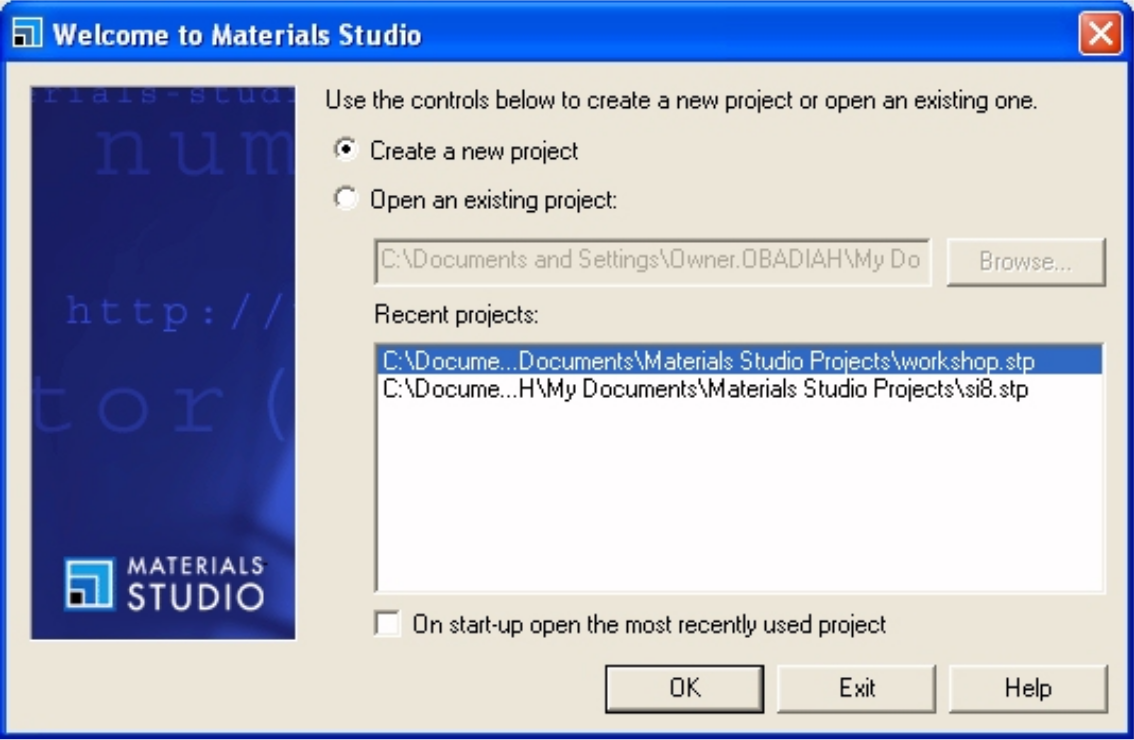
\includegraphics[height=2.70in,width=4.10in,viewport=0 0 1134 740,clip]{Figures/MS-New_Project-01.png}
\caption{\tiny \textrm{Quick Start for Materials studio:~Step-01.}}%(与文献\cite{EPJB33-47_2003}图1对比)
\label{MS-Quick_Start-01}
\end{figure}
}

\frame
{
	\frametitle{\textrm{MS:~Quick Start-02}}
\begin{figure}[h!]
\centering
\vspace*{-0.10in}
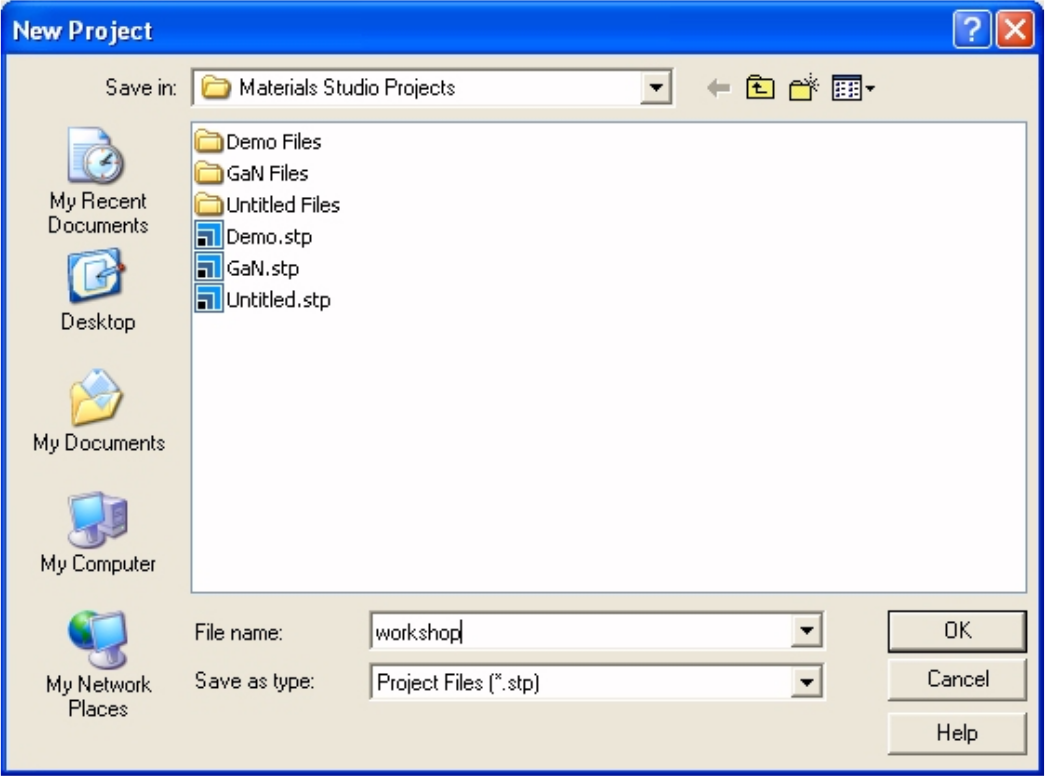
\includegraphics[height=2.70in,width=4.00in,viewport=0 0 1045 776,clip]{Figures/MS-New_Project-02.png}
\caption{\tiny \textrm{Quick Start for Materials studio:~Step-02.}}%(与文献\cite{EPJB33-47_2003}图1对比)
\label{MS-Quick_Start-02}
\end{figure}
}

\frame
{
	\frametitle{\textrm{MS:~Quick Start-03}}
\begin{figure}[h!]
\centering
\vspace*{-0.10in}
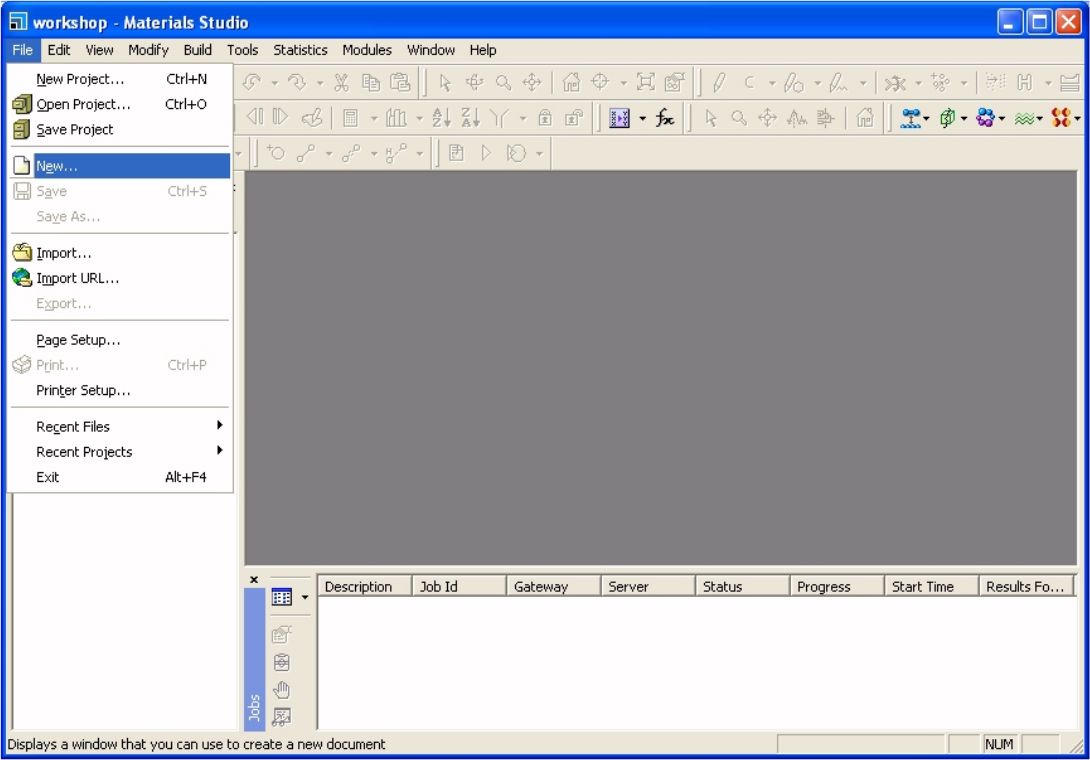
\includegraphics[height=2.68in,width=4.00in,viewport=0 0 1090 760,clip]{Figures/MS-New_Project-03.png}
\caption{\tiny \textrm{Quick Start for Materials studio:~Step-03.}}%(与文献\cite{EPJB33-47_2003}图1对比)
\label{MS-Quick_Start-03}
\end{figure}
}

%\subsection{\rm{Materials Studio:~Modelling}}
\frame
{
	\frametitle{\textrm{MS:~Quick Start-Modelling-01}}
\begin{figure}[h!]
\centering
\vspace*{-0.10in}
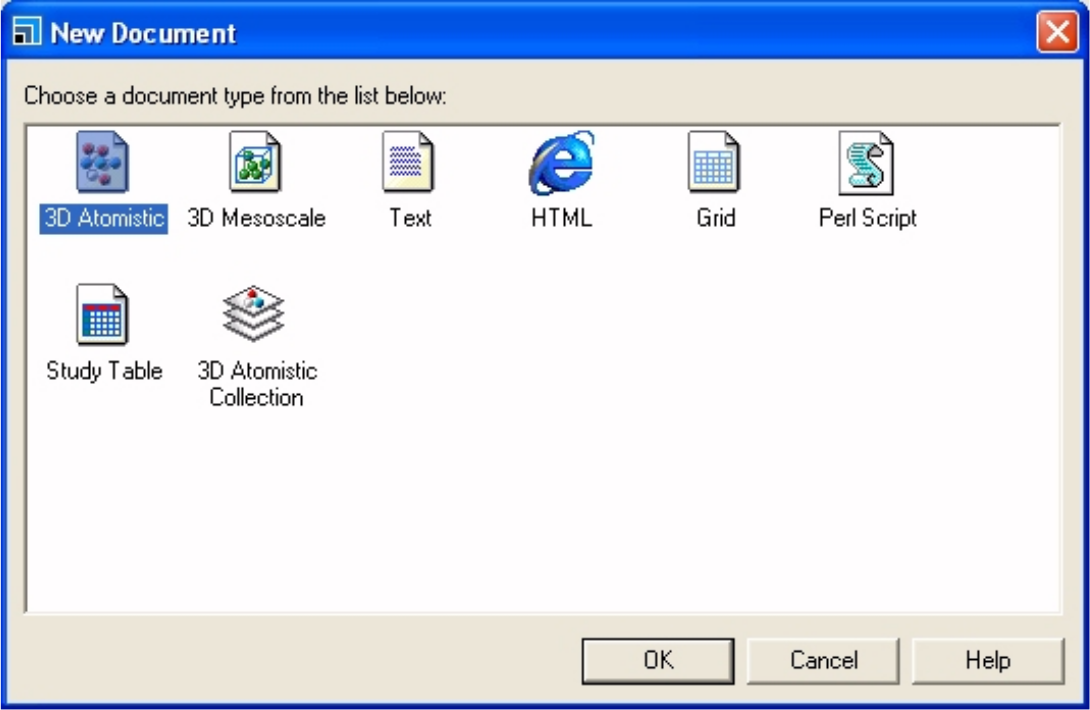
\includegraphics[height=2.60in,width=4.00in,viewport=0 0 1090 710,clip]{Figures/MS-New_Project-04.png}
\caption{\tiny \textrm{Quick Start for Materials studio:~Modelling-01.}}%(与文献\cite{EPJB33-47_2003}图1对比)
\label{MS-Quick_Start-Modelling-01}
\end{figure}
}

\frame
{
	\frametitle{\textrm{MS:~Quick Start-Modelling-02}}
\begin{figure}[h!]
\centering
\vspace*{-0.10in}
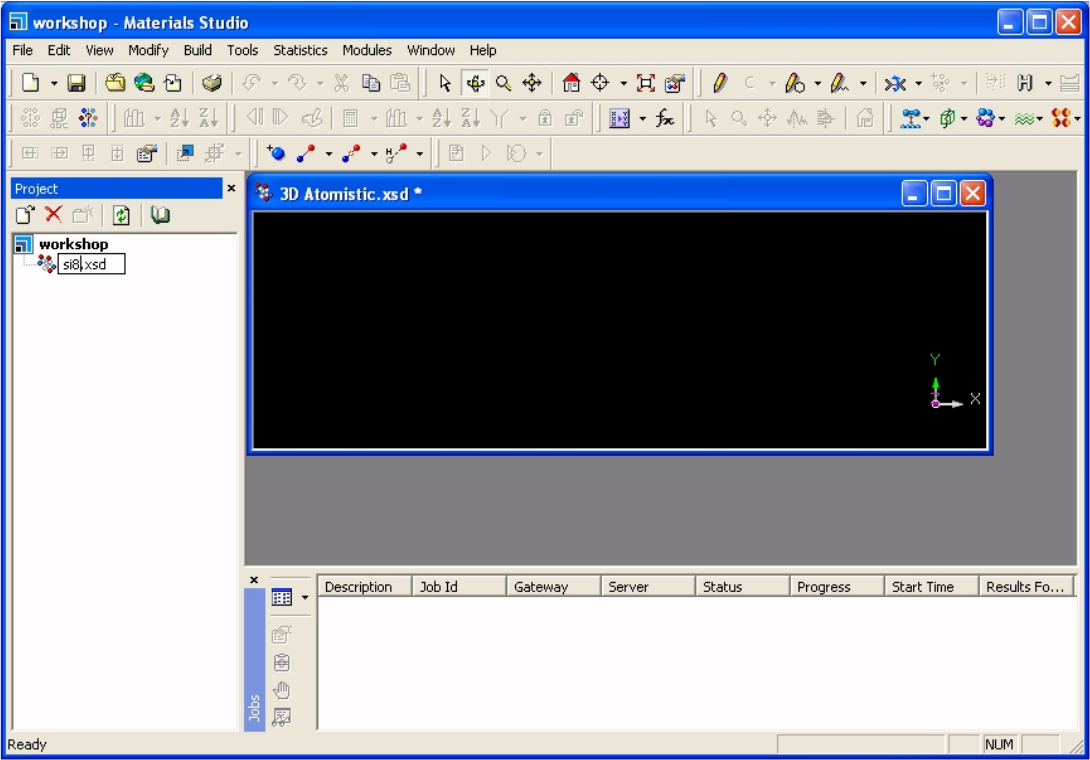
\includegraphics[height=2.68in,width=4.00in,viewport=0 0 1090 760,clip]{Figures/MS-New_Project-05.png}
\caption{\tiny \textrm{Quick Start for Materials studio:~Modelling-02.}}%(与文献\cite{EPJB33-47_2003}图1对比)
\label{MS-Quick_Start-Modelling-02}
\end{figure}
}

\frame
{
	\frametitle{\textrm{MS:~Modelling Crystal-01}}
\begin{figure}[h!]
\centering
\vspace*{-0.10in}
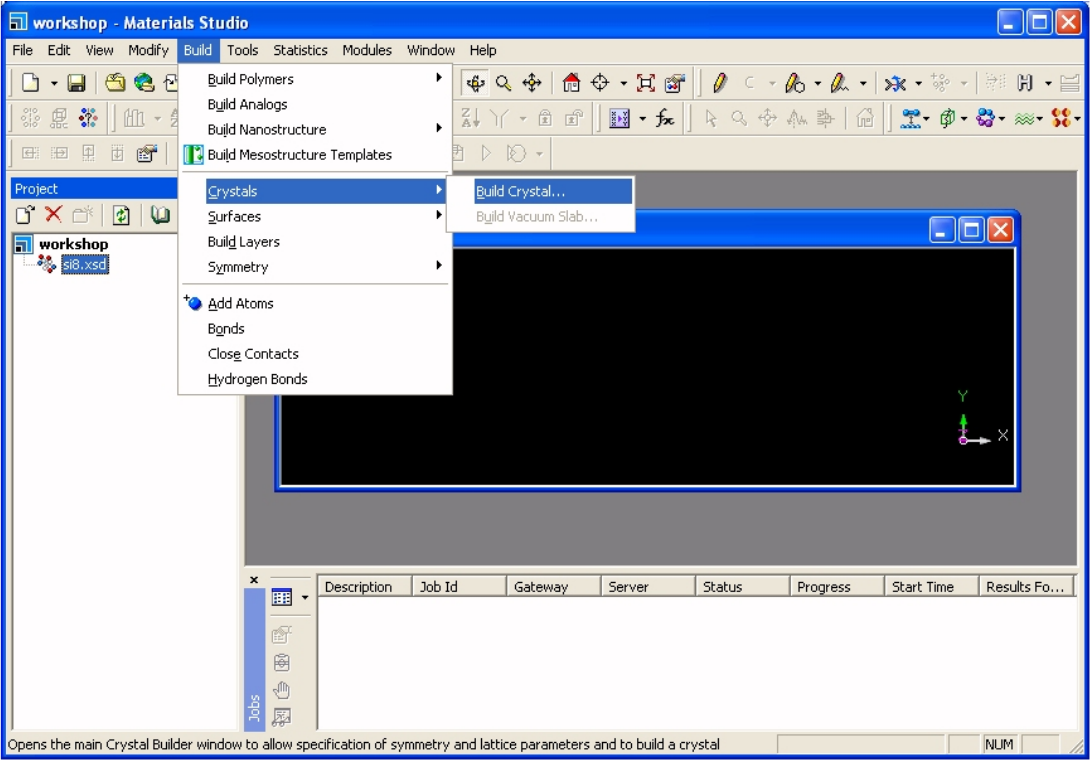
\includegraphics[height=2.68in,width=4.00in,viewport=0 0 1090 760,clip]{Figures/MS-New_Project-06.png}
\caption{\tiny \textrm{Modelling crystal by Materials studio.}}%(与文献\cite{EPJB33-47_2003}图1对比)
\label{MS-Modelling-Crystal-01}
\end{figure}
}

\frame
{
	\frametitle{\textrm{MS:~Modelling Crystal-02}}
\begin{figure}[h!]
\centering
\vspace*{-0.15in}
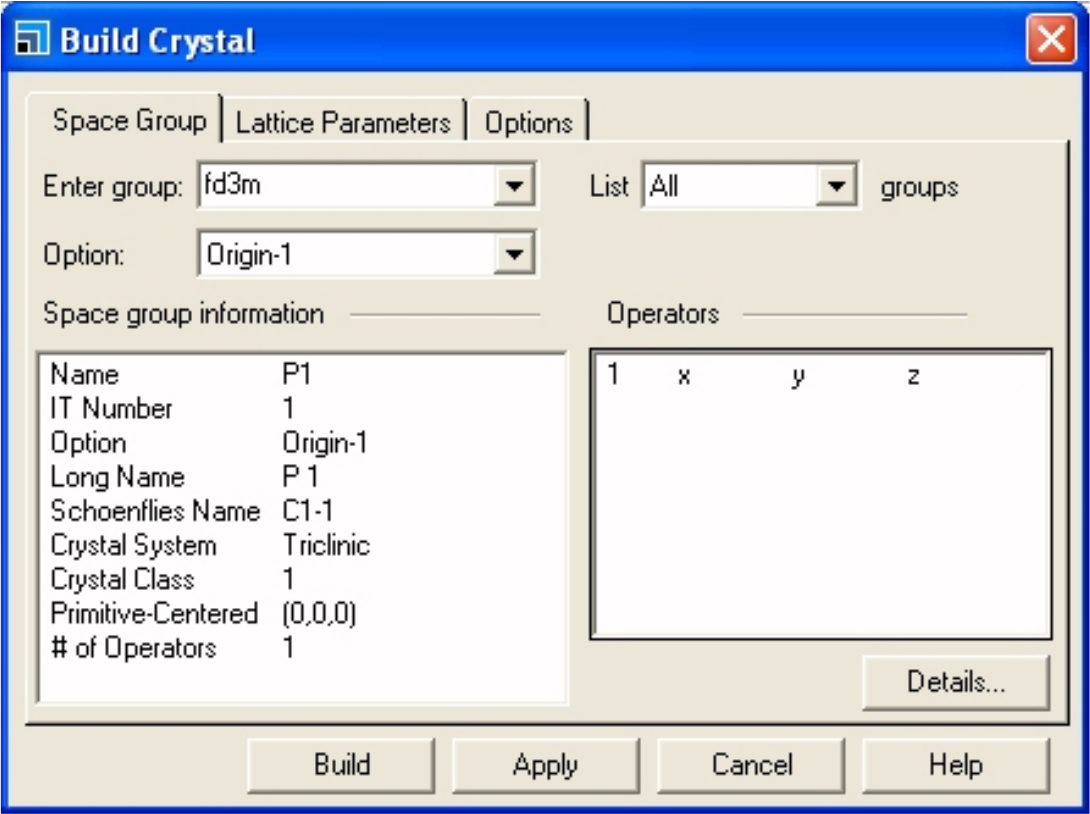
\includegraphics[height=2.75in,width=4.00in,viewport=0 0 1090 814,clip]{Figures/MS-New_Project-07.png}
\caption{\tiny \textrm{Modelling crystal by Materials studio:~Parameters.}}%(与文献\cite{EPJB33-47_2003}图1对比)
\label{MS-Modelling-Crystal-02}
\end{figure}
}

\subsection{\rm{Materials~Studio}建模}
\frame
{
	\frametitle{\textrm{MS~Modelling:~Polymers}}
\begin{figure}[h!]
\centering
\vspace*{-0.05in}
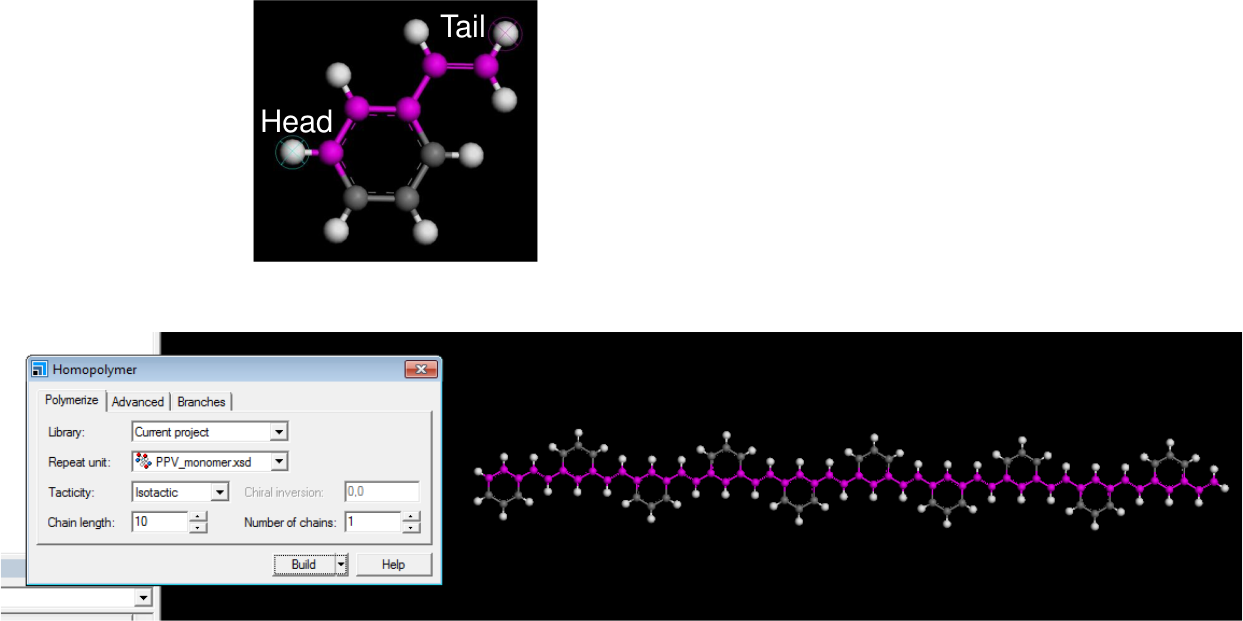
\includegraphics[height=2.10in,width=4.00in,viewport=0 0 1280 650,clip]{Figures/MS-Building_homopolymer.png}
\caption{\tiny \textrm{Building homopolymer for Materials studio.}}%(与文献\cite{EPJB33-47_2003}图1对比)
\label{MS-Building_homopolymer}
\end{figure}
}

\frame
{
	\frametitle{\textrm{MS~Modelling:~Polymers}}
\begin{figure}[h!]
\centering
\vspace*{-0.05in}
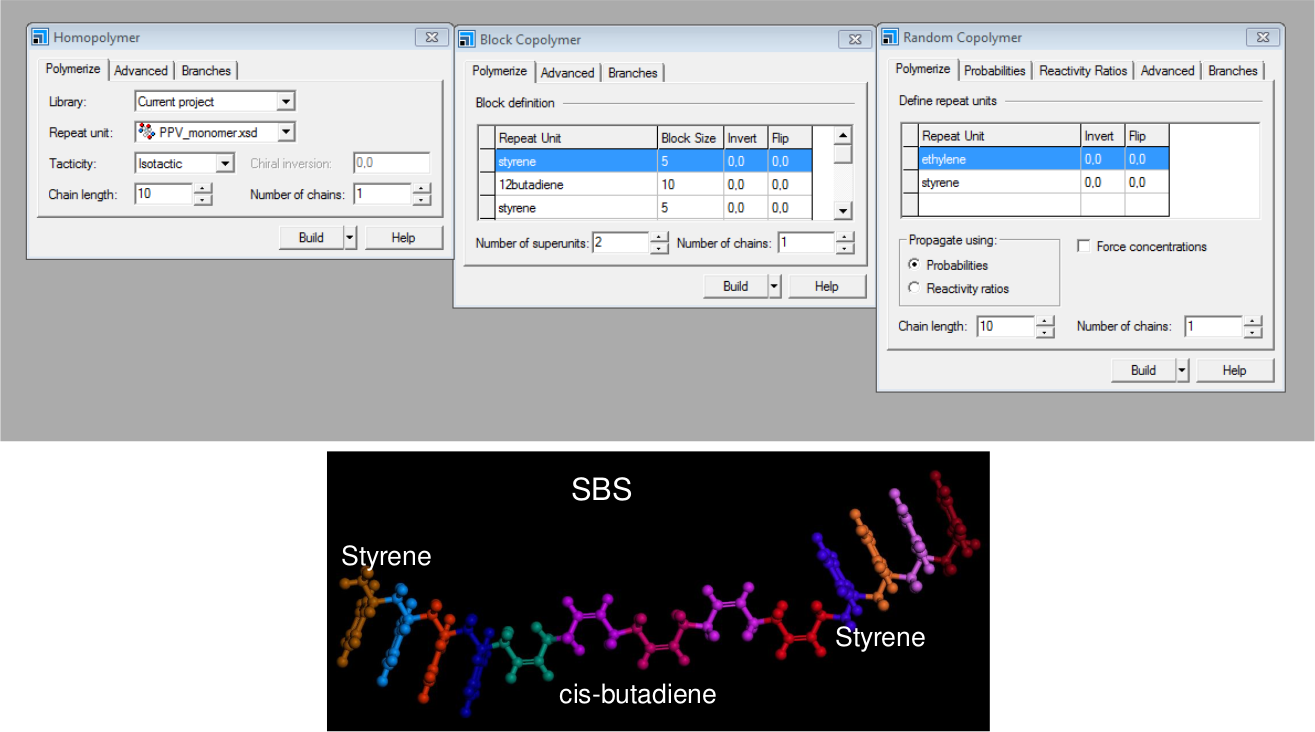
\includegraphics[height=2.20in,width=4.00in,viewport=0 0 1350 740,clip]{Figures/MS-Building_multypolymer.png}
\caption{\tiny \textrm{Building multi-polymer for Materials studio.}}%(与文献\cite{EPJB33-47_2003}图1对比)
\label{MS-Building_multypolymer}
\end{figure}
}

\frame
{
	\frametitle{\textrm{MS~Modelling:~amidoamine}}
\begin{figure}[h!]
\centering
\vspace*{-0.10in}
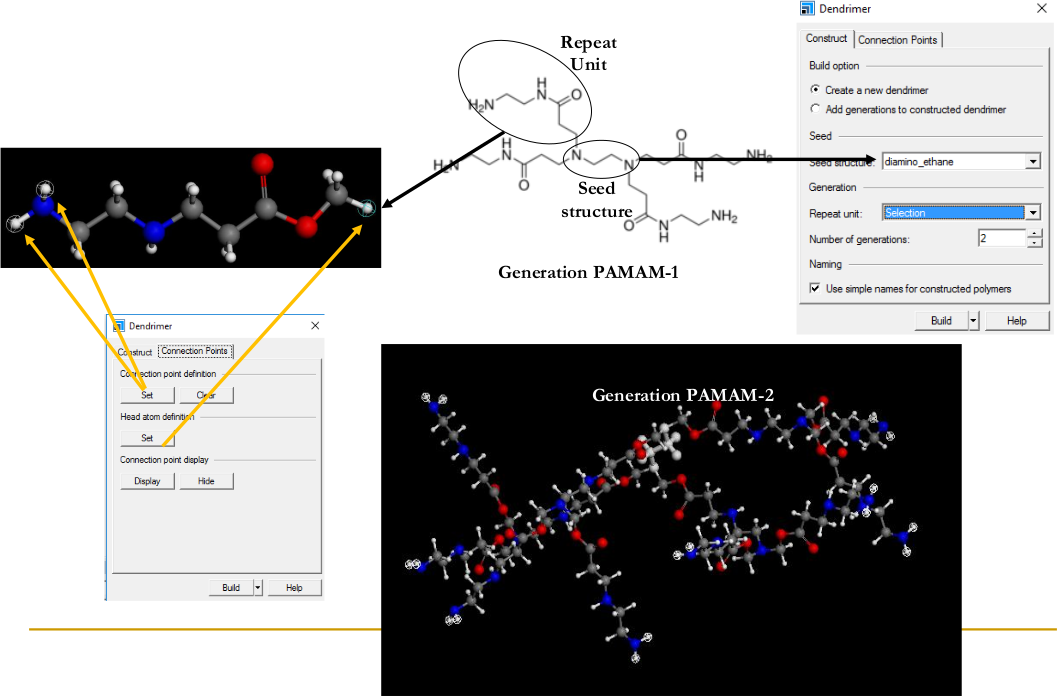
\includegraphics[height=2.45in,width=4.00in,viewport=0 0 1050 700,clip]{Figures/MS-Building_dendrimer.png}
\caption{\tiny \textrm{Building Poly-amidoamine (PAMAM) for Materials studio.}}%(与文献\cite{EPJB33-47_2003}图1对比)
\label{MS-Building_dendrimer}
\end{figure}
}

\frame
{
	\frametitle{\textrm{MS~Modelling:~from similar}}
\begin{figure}[h!]
\centering
\vspace*{-0.16in}
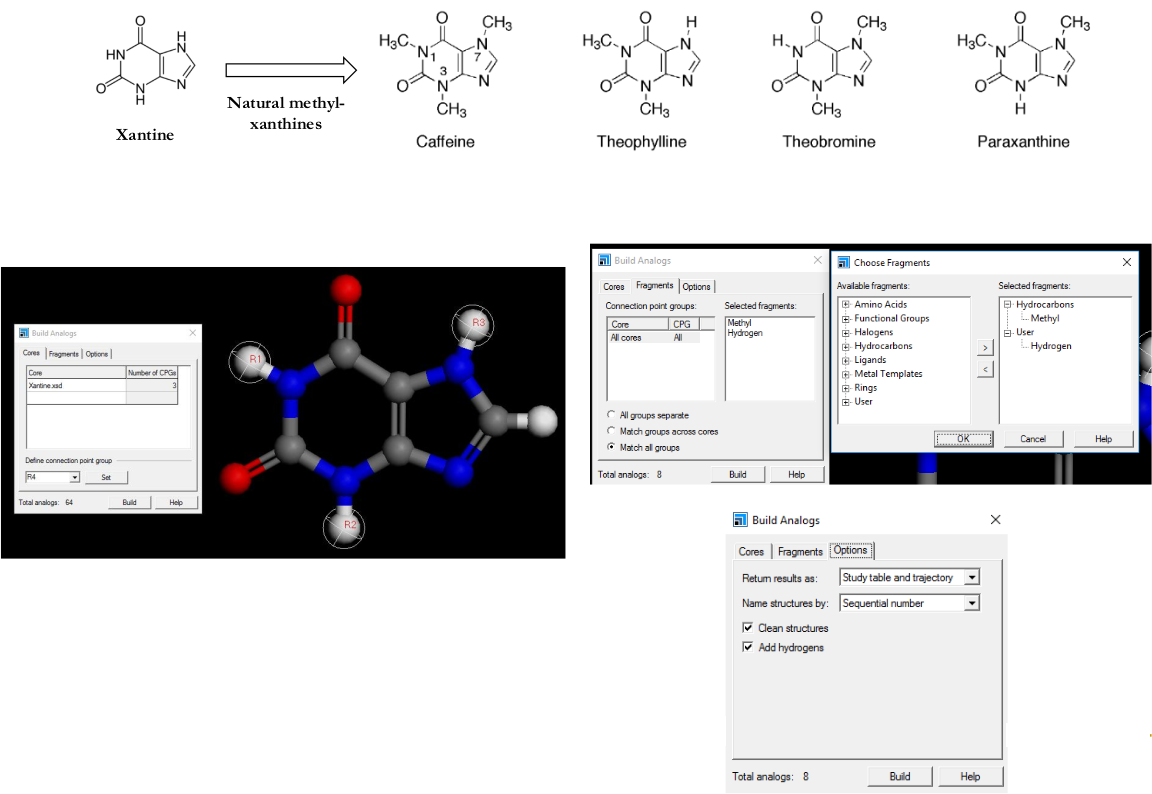
\includegraphics[height=2.65in,width=4.00in,viewport=0 0 1150 800,clip]{Figures/MS-Building_Analogs.png}
\caption{\tiny \textrm{Building from similar structure for Materials studio.}}%(与文献\cite{EPJB33-47_2003}图1对比)
\label{MS-Building_analogs}
\end{figure}
}

\frame
{
	\frametitle{\textrm{MS~Modelling:~from similar}}
\begin{figure}[h!]
\centering
%\vspace*{-0.10in}
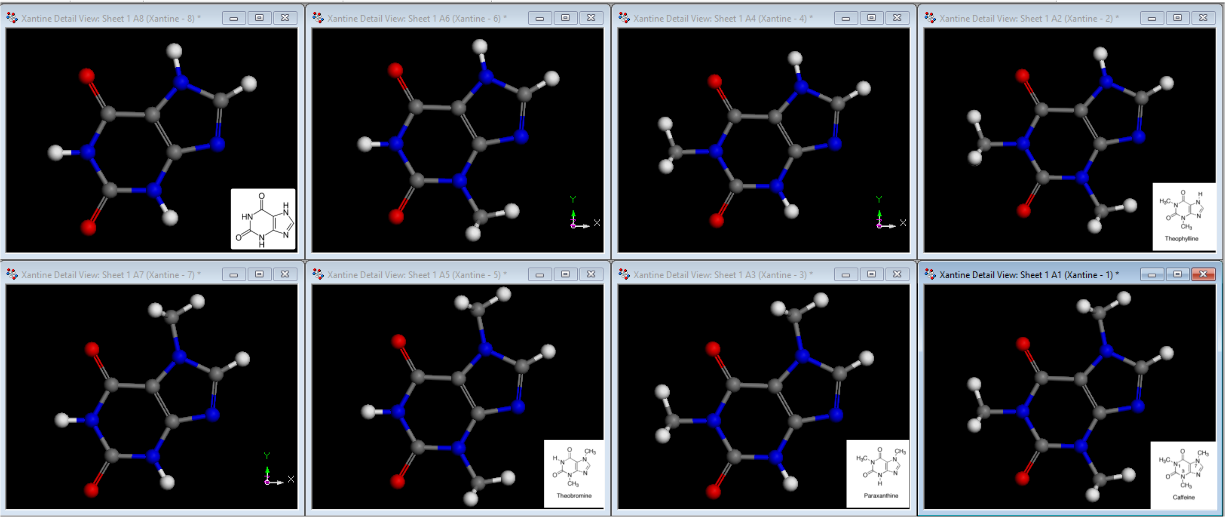
\includegraphics[height=1.70in,width=4.00in,viewport=0 0 1225 517,clip]{Figures/MS-Building_Analogs-examples.png}
\caption{\tiny \textrm{The similar structures in Materials studio.}}%(与文献\cite{EPJB33-47_2003}图1对比)
\label{MS-Building_analogs-examples}
\end{figure}
}

\frame
{
	\frametitle{\textrm{MS~Modelling:~Single-wall Nanotubes}}
\begin{figure}[h!]
\centering
\vspace*{-0.16in}
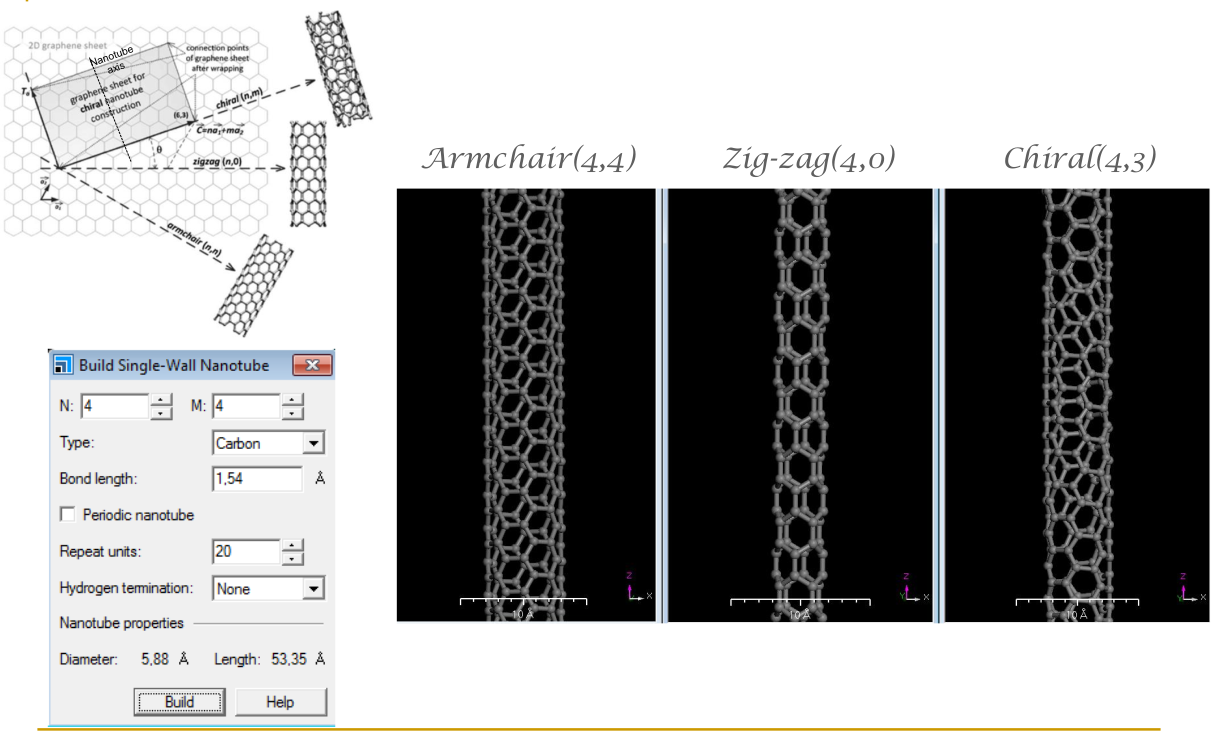
\includegraphics[height=2.60in,width=4.00in,viewport=0 0 1211 731,clip]{Figures/MS-Building_Single_wall-nanotube.png}
\caption{\tiny \textrm{Building Single-wall Nanotubes for Materials studio.}}%(与文献\cite{EPJB33-47_2003}图1对比)
\label{MS-Building_Single_wall-Nanotubes}
\end{figure}
}

\frame
{
	\frametitle{\textrm{MS~Modelling:~Single-wall Nanotubes}}
\begin{figure}[h!]
\centering
%\vspace*{-0.00in}
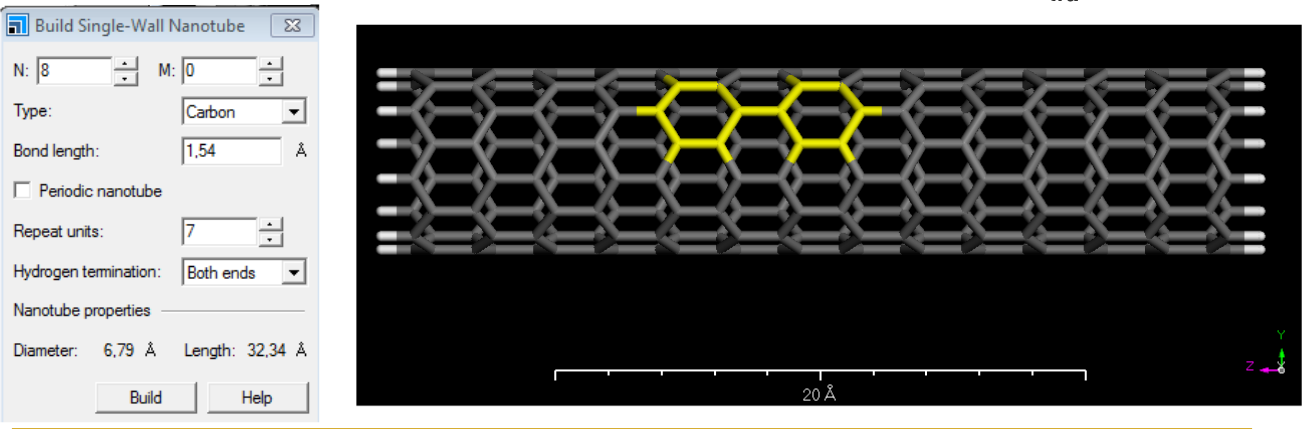
\includegraphics[height=1.32in,width=4.00in,viewport=0 0 1302 429,clip]{Figures/MS-Building_Single_wall-nanotube-example.png}
\caption{\tiny \textrm{Building Single-wall Nanobubes:~Select atoms for Materials studio.}}%(与文献\cite{EPJB33-47_2003}图1对比)
\label{MS-Building_Single_wall-Nanotubes-example}
\end{figure}
}

\frame
{
	\frametitle{\textrm{MS~Modelling:~Multi-wall Nanotubes}}
\begin{figure}[h!]
\centering
\vspace*{-0.16in}
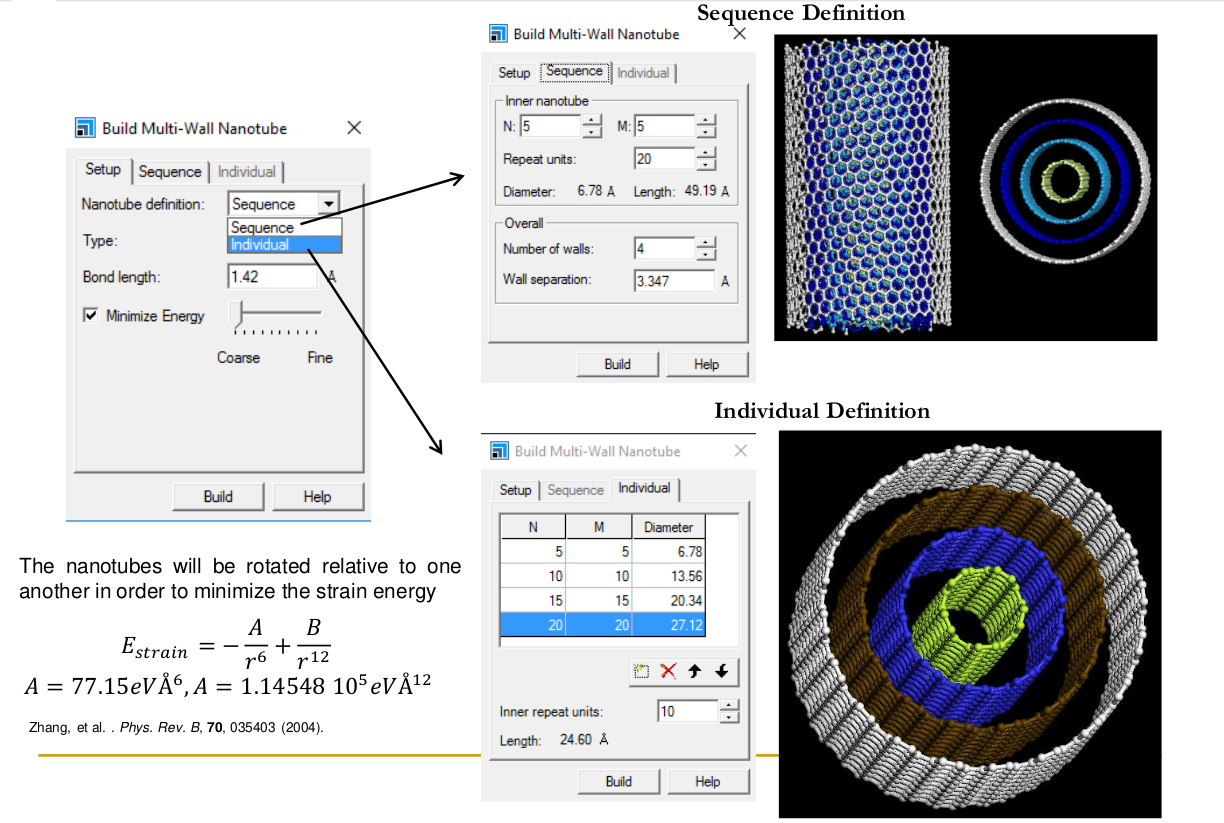
\includegraphics[height=2.68in,width=4.00in,viewport=0 0 1224 823,clip]{Figures/MS-Building_Multi_wall-nanotube.png}
\caption{\tiny \textrm{Building Multi-wall Nanotubes for Materials studio.}}%(与文献\cite{EPJB33-47_2003}图1对比)
\label{MS-Building_Multi_wall-Nanotubes}
\end{figure}
}

\frame
{
	\frametitle{\textrm{MS~Modelling:~Single-wall Nanotubes bundle}}
\begin{figure}[h!]
\centering
\vspace*{-0.18in}
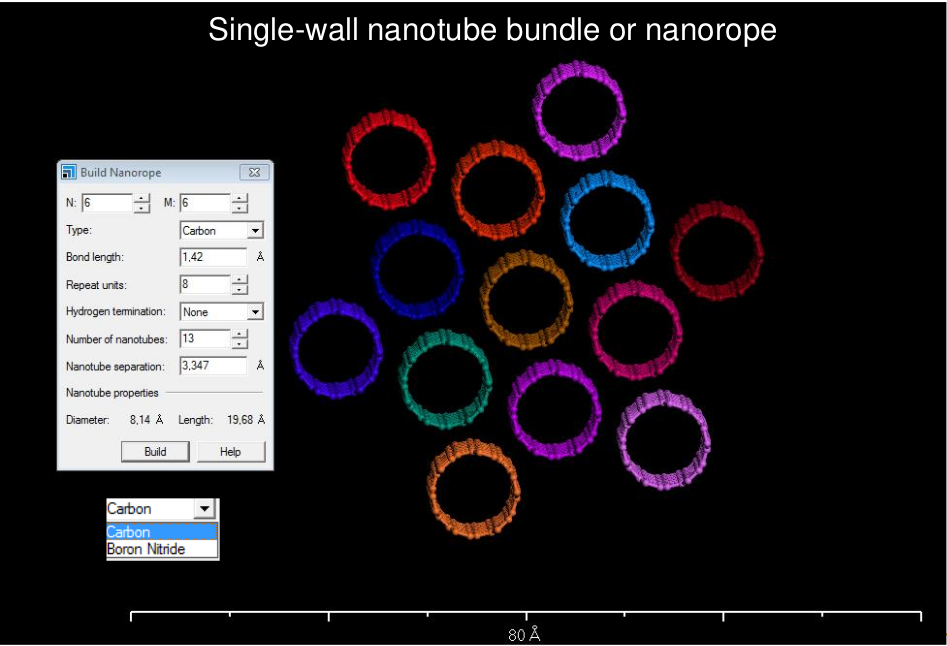
\includegraphics[height=2.70in,width=4.00in,viewport=0 0 947 646,clip]{Figures/MS-Building_Nanorope.png}
\caption{\tiny \textrm{Building Single-wall Nanotube bundle or nanorope for Materials studio.}}%(与文献\cite{EPJB33-47_2003}图1对比)
\label{MS-Building_Nanorope-bundle}
\end{figure}
}

\frame
{
	\frametitle{\textrm{MS~Modelling:~Construction of Nanocluster}}
\begin{figure}[h!]
\centering
\vspace*{-0.15in}
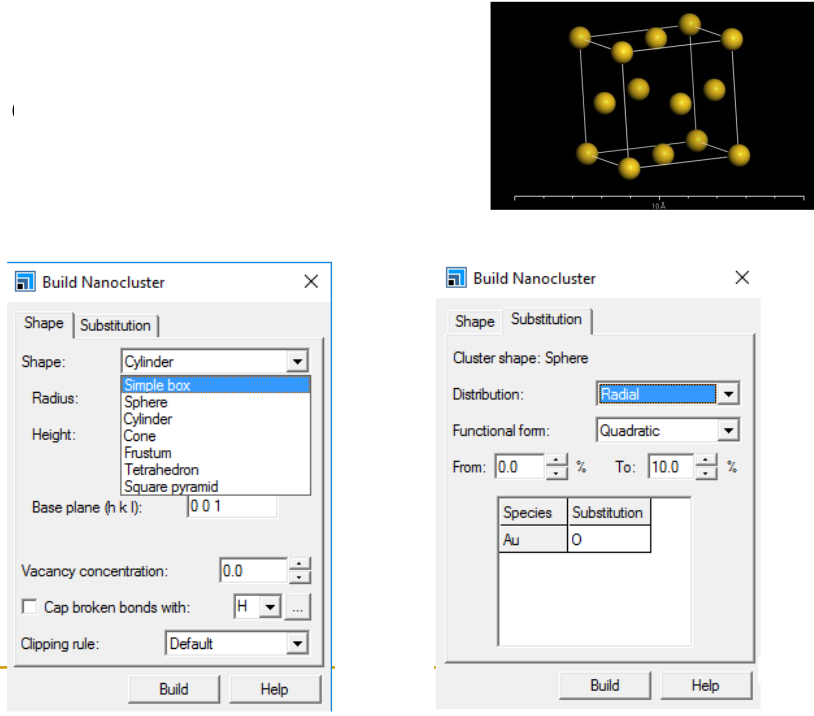
\includegraphics[height=2.45in,width=2.90in,viewport=0 0 814 716,clip]{Figures/MS-Building_Nanocluster.png}
\caption{\tiny \textrm{Building of Nanocluster for Materials studio.}}%(与文献\cite{EPJB33-47_2003}图1对比)
\label{MS-Building_Nanocluster}
\end{figure}
}

\frame
{
	\frametitle{\textrm{MS~Modelling:~Construction of Nanocluster}}
\begin{figure}[h!]
\centering
\vspace*{-0.10in}
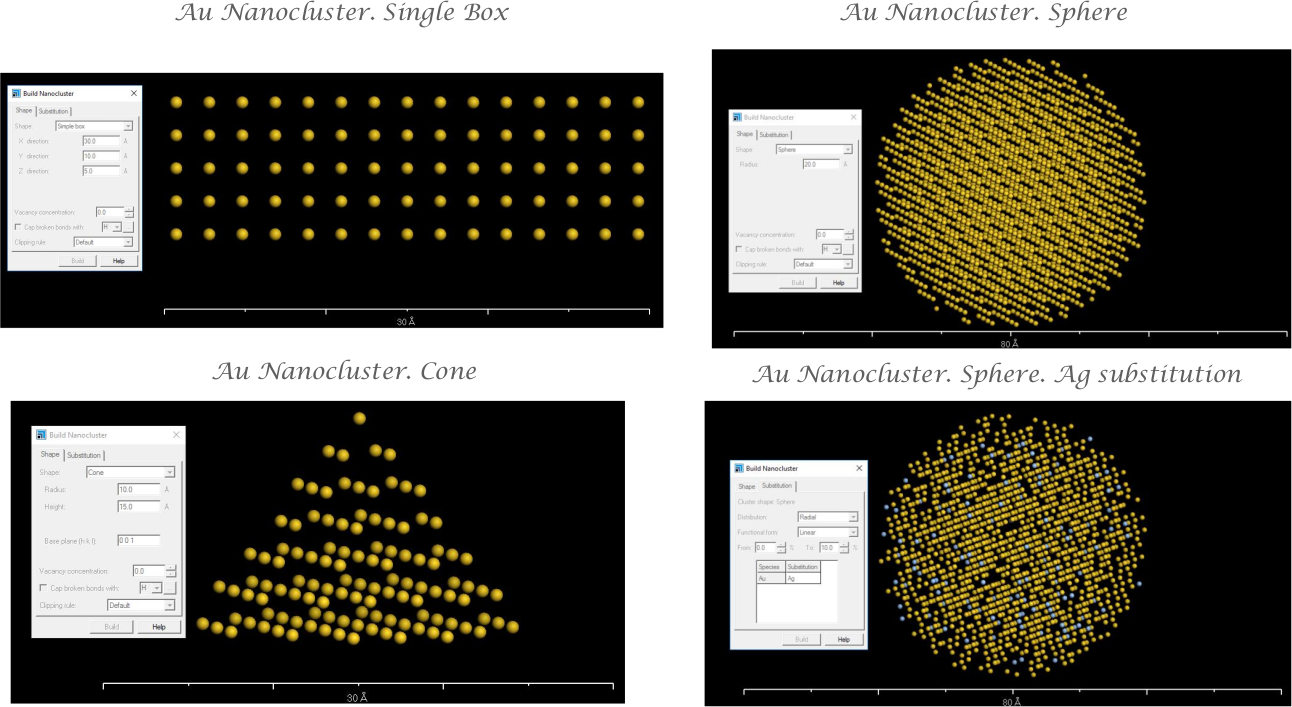
\includegraphics[height=2.20in,width=4.00in,viewport=0 0 1292 707,clip]{Figures/MS-Building_Nanocluster-examples.png}
\caption{\tiny \textrm{The Nanocluster structures in Materials studio.}}%(与文献\cite{EPJB33-47_2003}图1对比)
\label{MS-Building_Nanocluster-examples}
\end{figure}
}

\frame
{
	\frametitle{\textrm{MS~Modelling:~Meso-molecules}}
\begin{figure}[h!]
\centering
\vspace*{-0.12in}
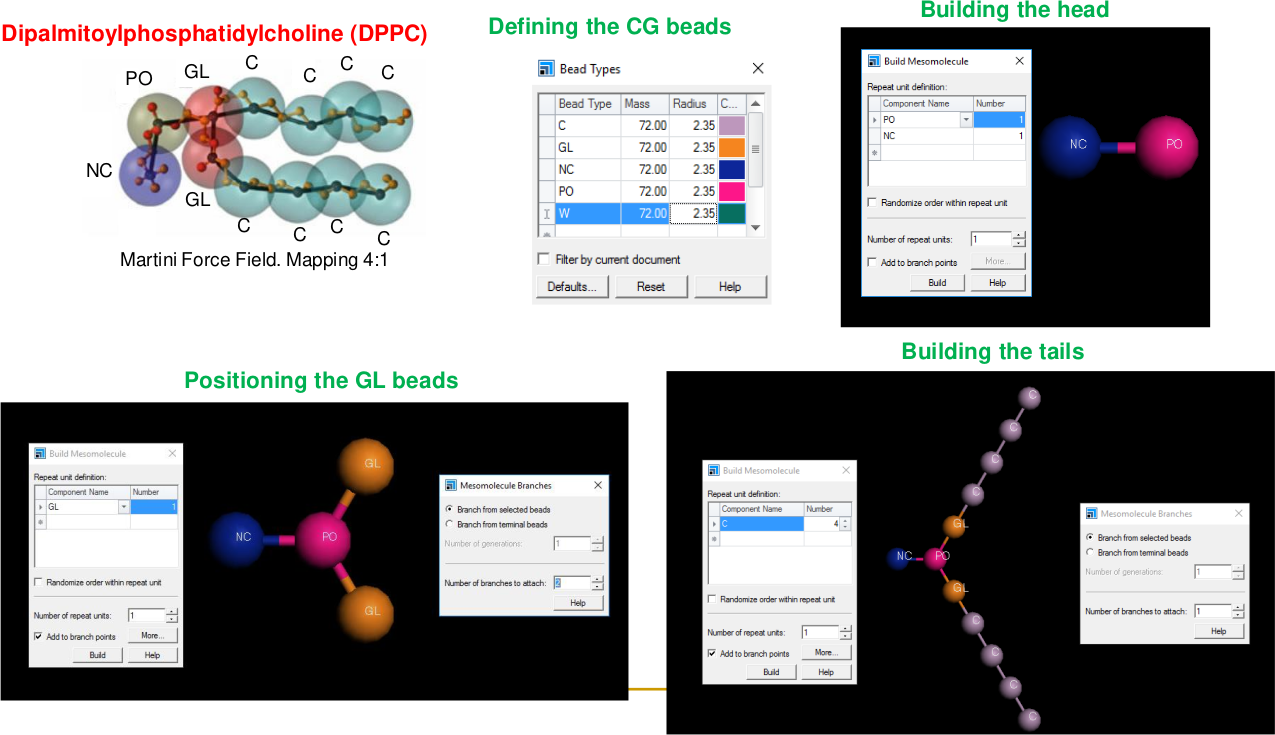
\includegraphics[height=2.31in,width=4.00in,viewport=0 0 1275 735,clip]{Figures/MS-Building_Mesomolecule.png}
\caption{\tiny \textrm{Building Meso-molecule structure for Materials studio.}}%(与文献\cite{EPJB33-47_2003}图1对比)
\label{MS-Building_Meso-molecules}
\end{figure}
}

\frame
{
	\frametitle{\textrm{MS~Modelling:~Meso-molecules by template}}
\begin{figure}[h!]
\centering
\vspace*{-0.12in}
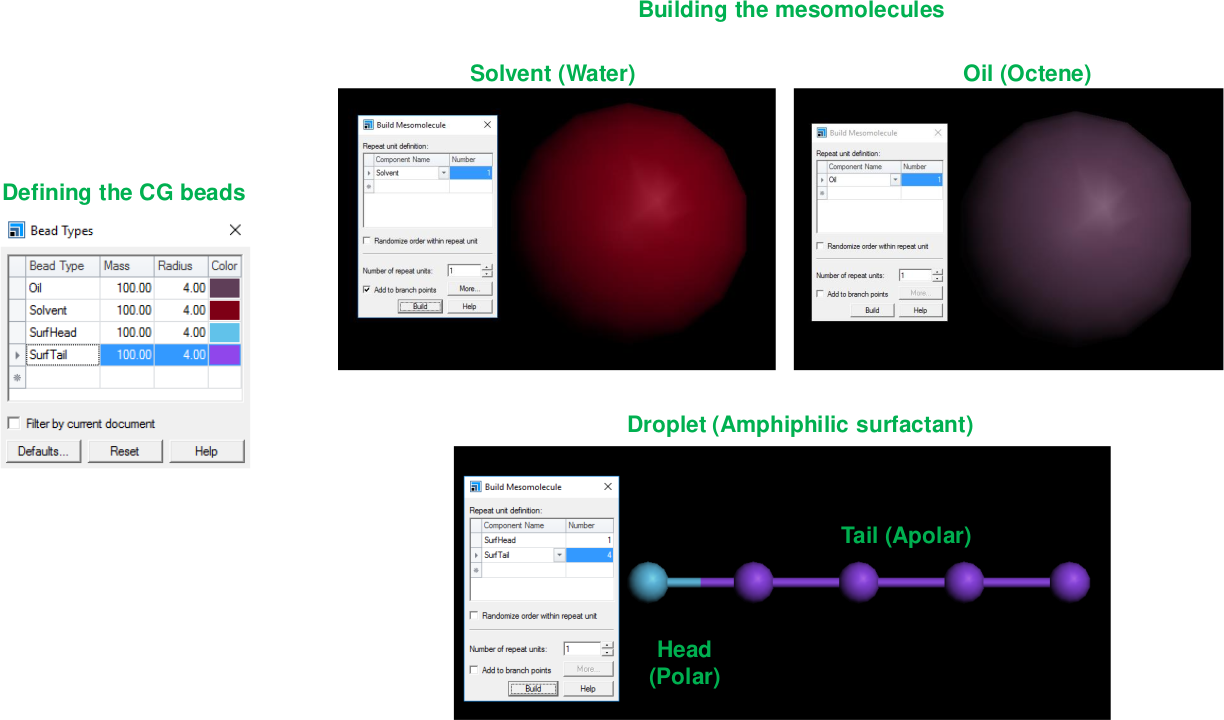
\includegraphics[height=2.36in,width=4.00in,viewport=0 0 1224 720,clip]{Figures/MS-Building_Mesomolecule-template.png}
\caption{\tiny \textrm{Building Meso-molecule by temlapte for Materials studio.}}%(与文献\cite{EPJB33-47_2003}图1对比)
\label{MS-Building_Meso-molecules-template}
\end{figure}
}

\frame
{
	\frametitle{\textrm{MS~Modelling:~Meso-molecules by template}}
\begin{figure}[h!]
\centering
\vspace*{-0.18in}
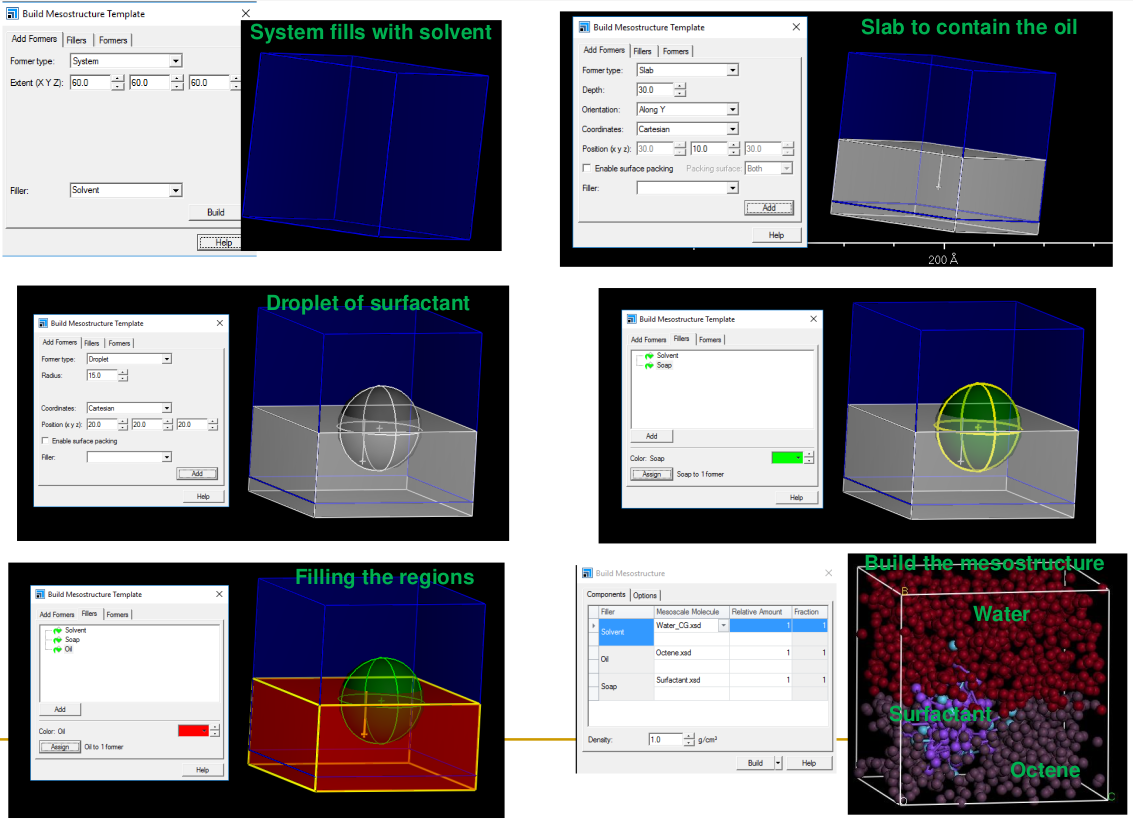
\includegraphics[height=2.70in,width=3.72in,viewport=0 0 1133 822,clip]{Figures/MS-Building_Mesomolecule-example.png}
\caption{\tiny \textrm{Building Meso-molecule by temlapte for Materials studio.}}%(与文献\cite{EPJB33-47_2003}图1对比)
\label{MS-Building_Meso-molecules-template-example}
\end{figure}
}

\frame
{
	\frametitle{\textrm{MS~Modelling:~MOF Crystals}}
\begin{figure}[h!]
\centering
\vspace*{-0.18in}
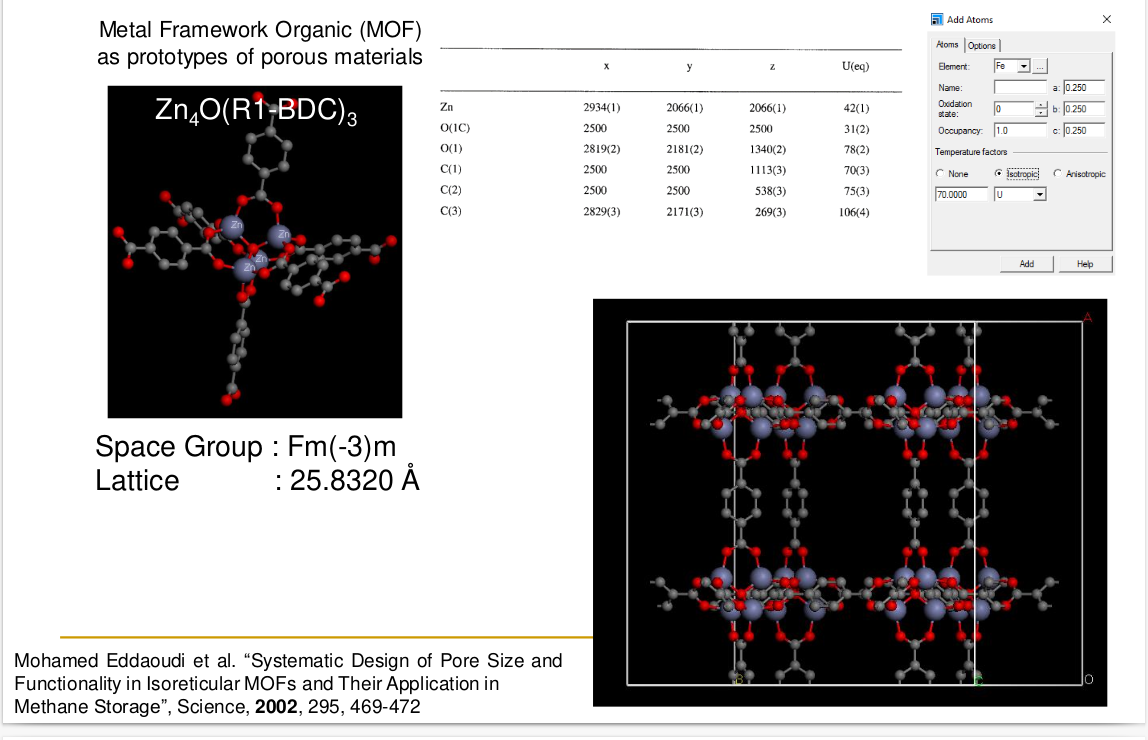
\includegraphics[height=2.60in,width=4.00in,viewport=0 0 1148 740,clip]{Figures/MS-Building_MOF.png}
\caption{\tiny \textrm{Building Metal Framework Orgainc (MOF) for Materials studio.}}%(与文献\cite{EPJB33-47_2003}图1对比)
\label{MS-Building_MOF}
\end{figure}
}

\frame
{
	\frametitle{\textrm{MS~Modelling:~Miller Planes in Crystals}}
\begin{figure}[h!]
\centering
\vspace*{-0.18in}
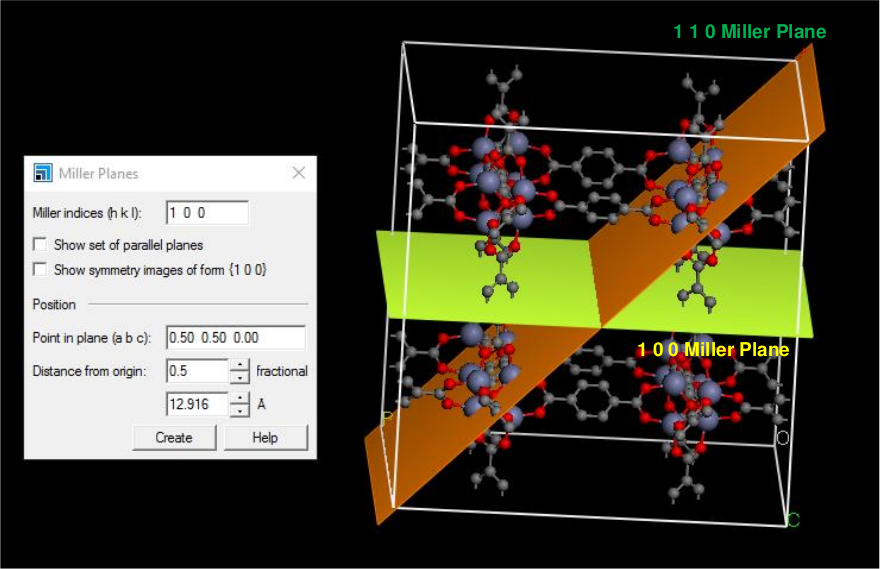
\includegraphics[height=2.60in,width=4.00in,viewport=0 0 880 569,clip]{Figures/MS-Building_Miller_Plane.png}
\caption{\tiny \textrm{Building Miller Planes in crystals for Materials studio.}}%(与文献\cite{EPJB33-47_2003}图1对比)
\label{MS-Building_Miller-Plane}
\end{figure}
}

\frame
{
	\frametitle{\textrm{MS~Modelling:~surface from Crystals}}
\begin{figure}[h!]
\centering
\vspace*{-0.10in}
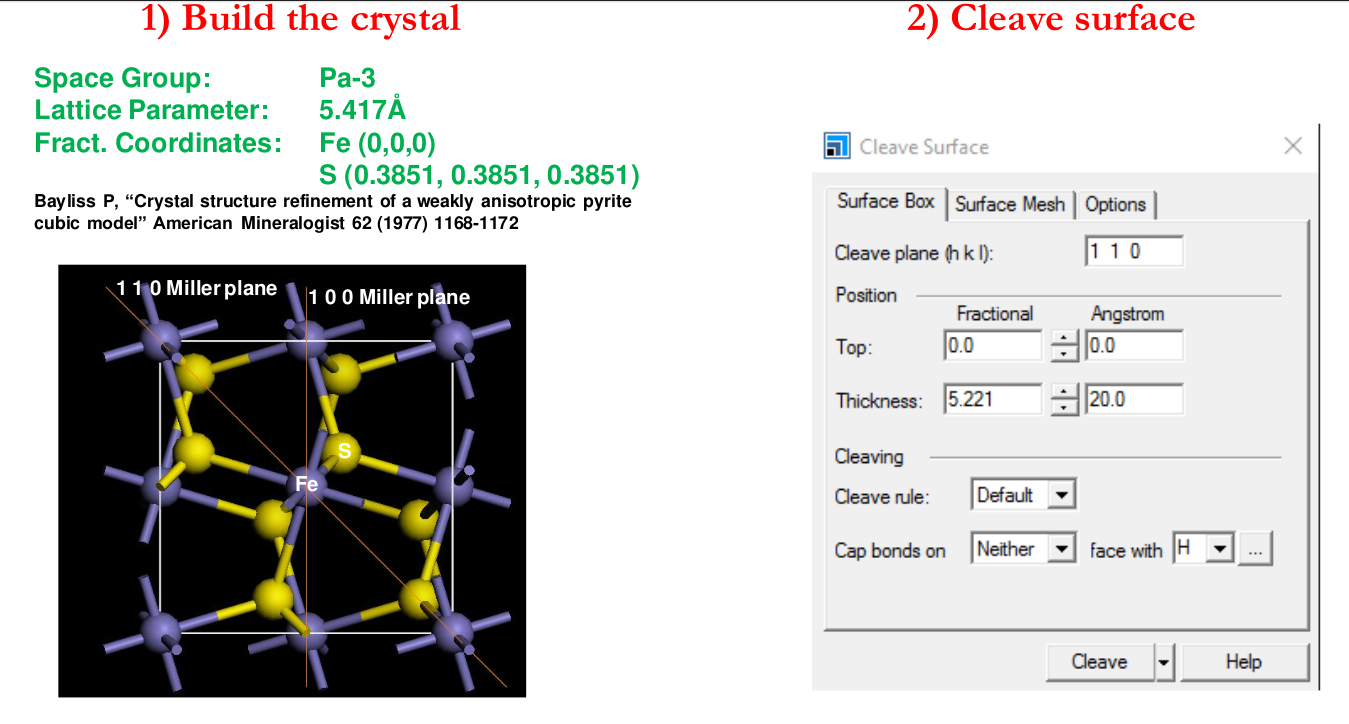
\includegraphics[height=2.20in,width=4.00in,viewport=0 0 1349 724,clip]{Figures/MS-Building_Cleave_Surface.png}
\caption{\tiny \textrm{Building surfaces from crystals for Materials studio.}}%(与文献\cite{EPJB33-47_2003}图1对比)
\label{MS-Building_Cleave_Surface}
\end{figure}
}

\frame
{
	\frametitle{\textrm{MS~Modelling:~surface in Crystals}}
\begin{figure}[h!]
\centering
\vspace*{-0.18in}
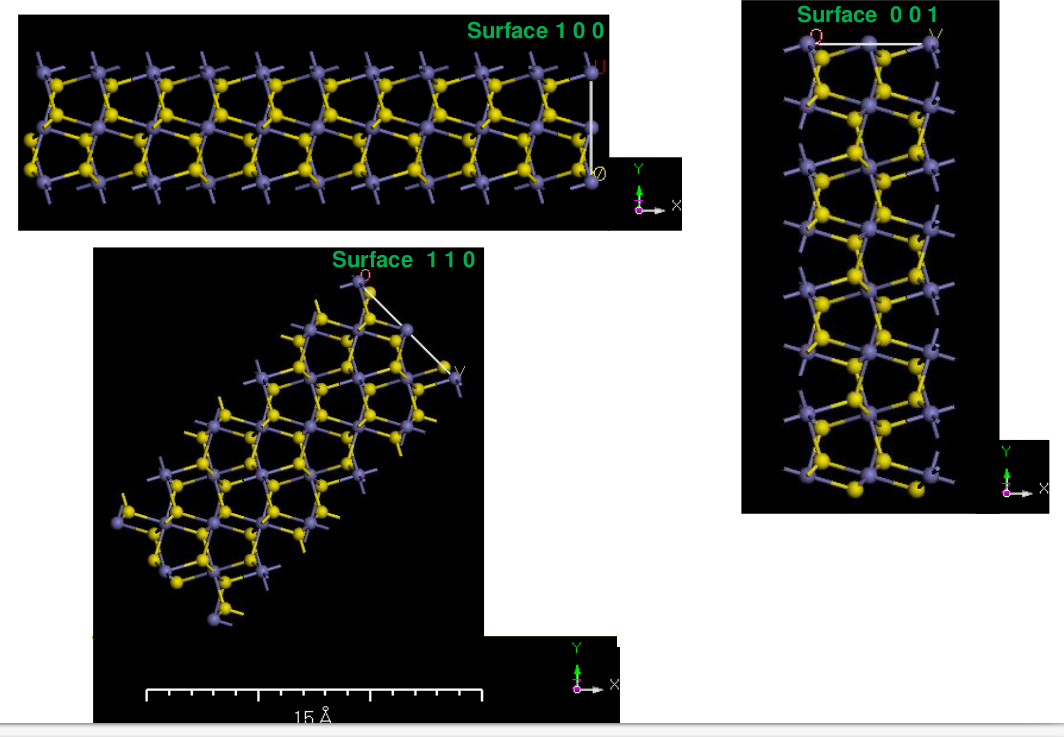
\includegraphics[height=2.70in,width=3.90in,viewport=0 0 1064 737,clip]{Figures/MS-Building_Surface.png}
\caption{\tiny \textrm{Building surfaces in crystals for Materials studio.}}%(与文献\cite{EPJB33-47_2003}图1对比)
\label{MS-Building_Surface}
\end{figure}
}

\frame
{
	\frametitle{\textrm{MS~Modelling:~layers and vacuum}}
\begin{figure}[h!]
\centering
\vspace*{-0.18in}
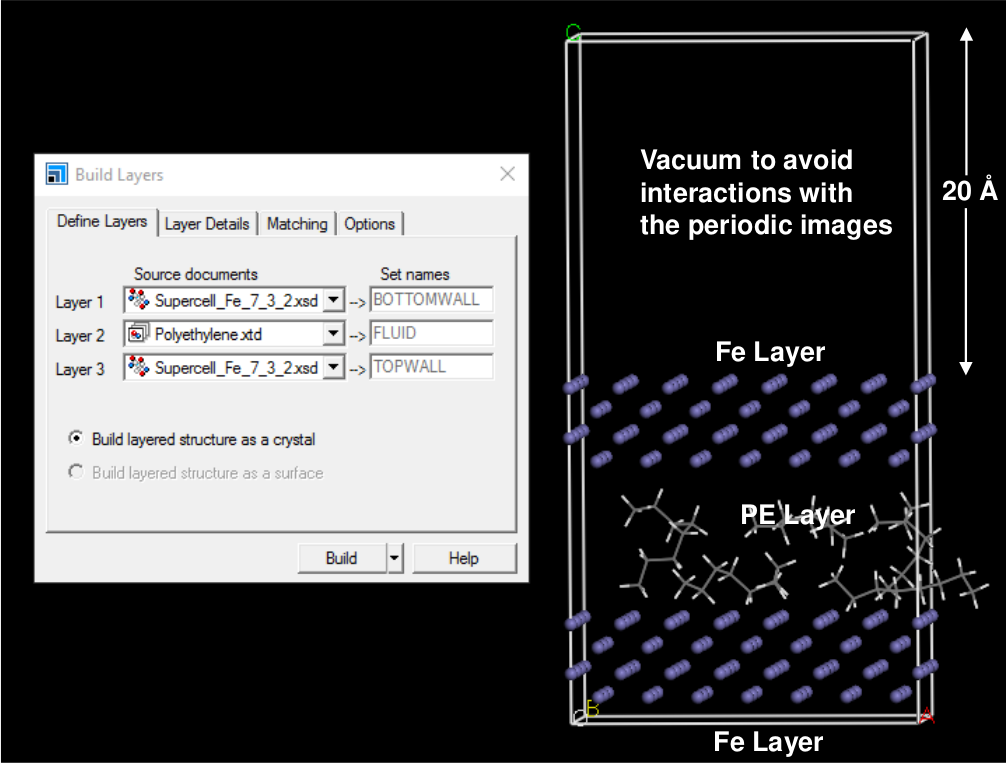
\includegraphics[height=2.70in,width=3.60in,viewport=0 0 1006 763,clip]{Figures/MS-Building_layer.png}
\caption{\tiny \textrm{Building metal-polymer-metal by multi-layers and vacuum for Materials studio.}}%(与文献\cite{EPJB33-47_2003}图1对比)
\label{MS-Building_layer}
\end{figure}
}

\frame
{
	\frametitle{\textrm{Quantum simulation:~Tools}}
\begin{figure}[h!]
\centering
\vspace*{-0.10in}
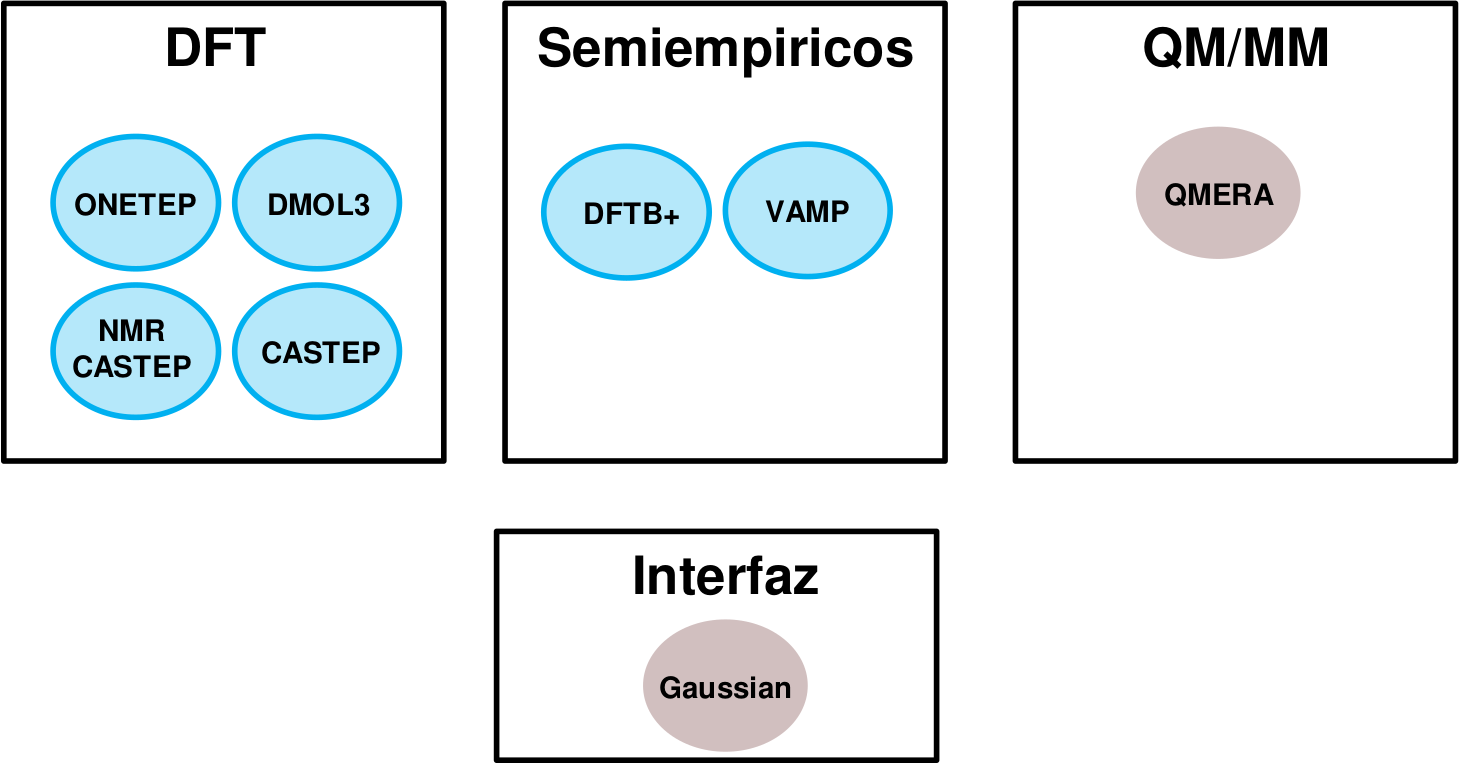
\includegraphics[height=2.10in,width=4.00in,viewport=0 0 1459 763,clip]{Figures/MS-Quantum_simulation-tools.png}
\caption{\tiny \textrm{Calculation modules for quantum simulation in Materials studio.}}%(与文献\cite{EPJB33-47_2003}图1对比)
\label{MS-Quantum_simulation}
\end{figure}
}

\frame
{
	\frametitle{\textrm{Ms~Calculation modules comparison}}
\begin{figure}[h!]
\centering
\vspace*{-0.10in}
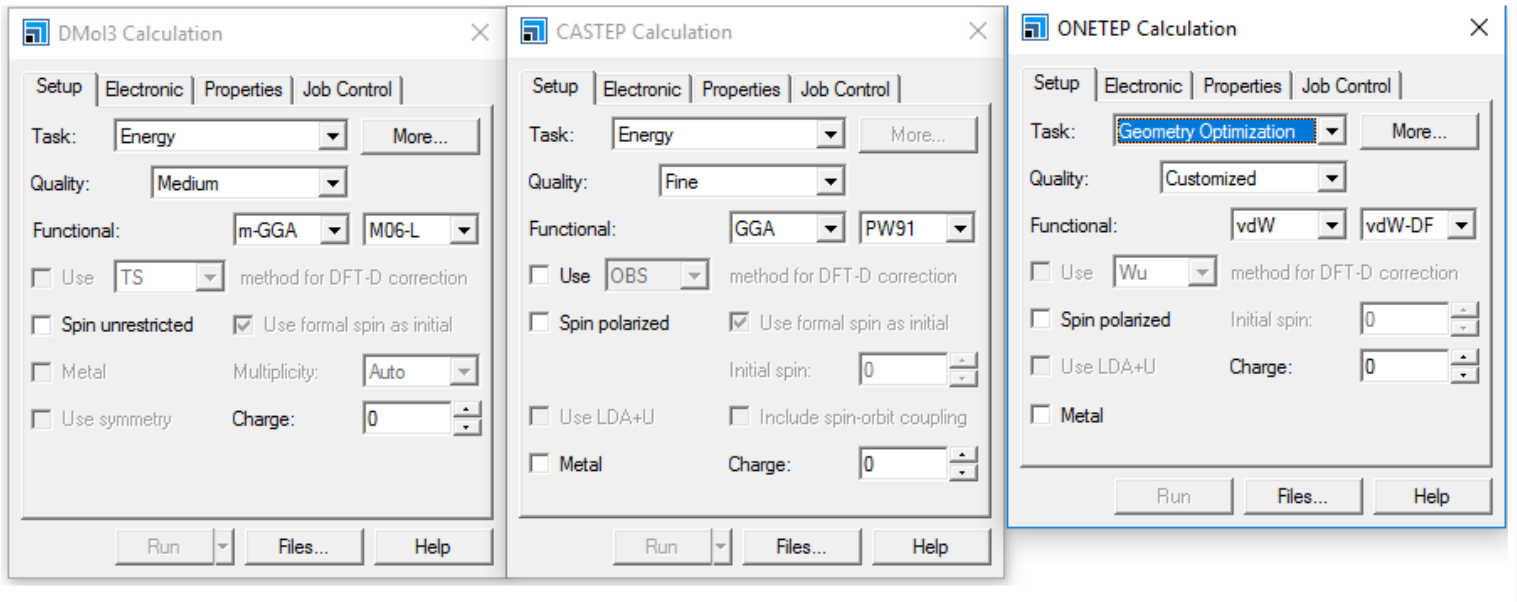
\includegraphics[height=1.60in,width=4.00in,viewport=0 0 1517 602,clip]{Figures/MS-Caluculator-compare-1.png}
\caption{\tiny \textrm{Calculation parameters comparison in Materials studio.}}%(与文献\cite{EPJB33-47_2003}图1对比)
\label{MS-Module_parameters}
\end{figure}
}

\frame
{
	\frametitle{\textrm{Ms~xc functional  comparison}}
\begin{figure}[h!]
\centering
\vspace*{-0.15in}
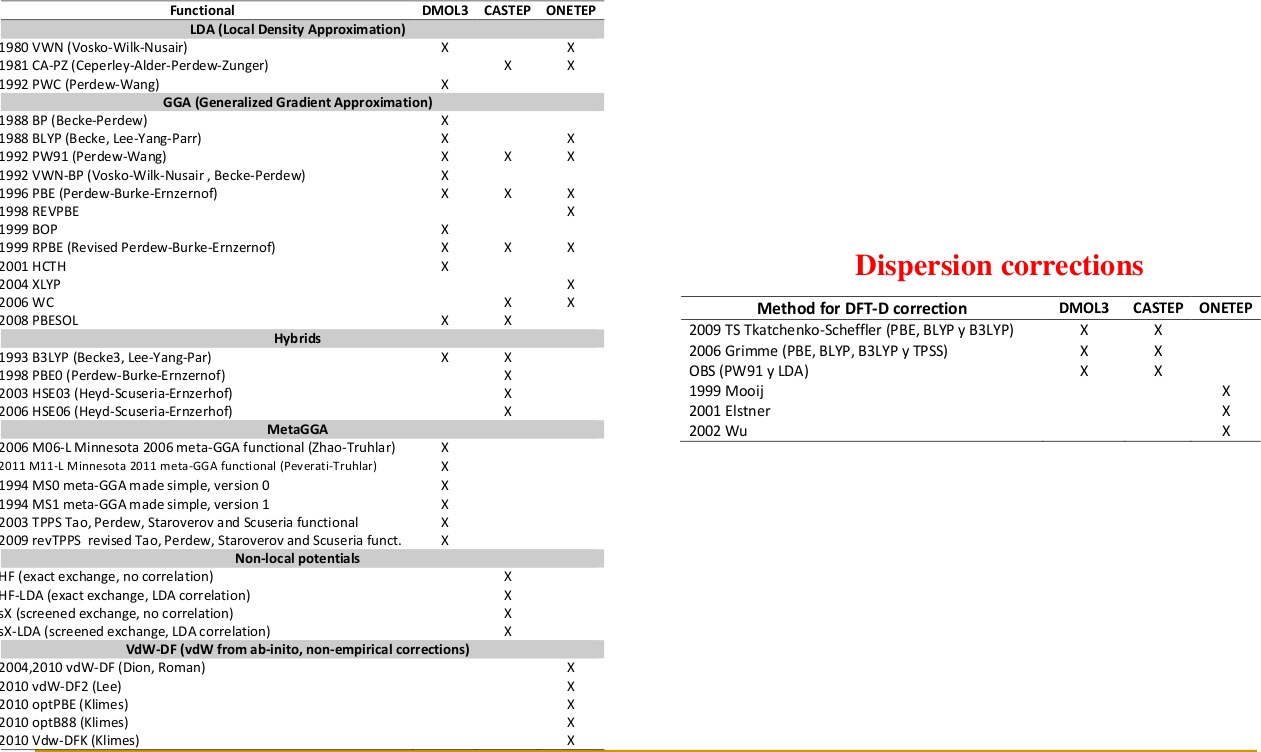
\includegraphics[height=2.40in,width=4.00in,viewport=0 0 1261 751,clip]{Figures/MS-xc_functional-compare.png}
\caption{\tiny \textrm{XC functional comparison in Materials studio.}}%(与文献\cite{EPJB33-47_2003}图1对比)
\label{MS-Module_xc-functional}
\end{figure}
}

\frame
{
	\frametitle{\textrm{Ms~Calculation modules comparison}}
\begin{figure}[h!]
\centering
\vspace*{-0.18in}
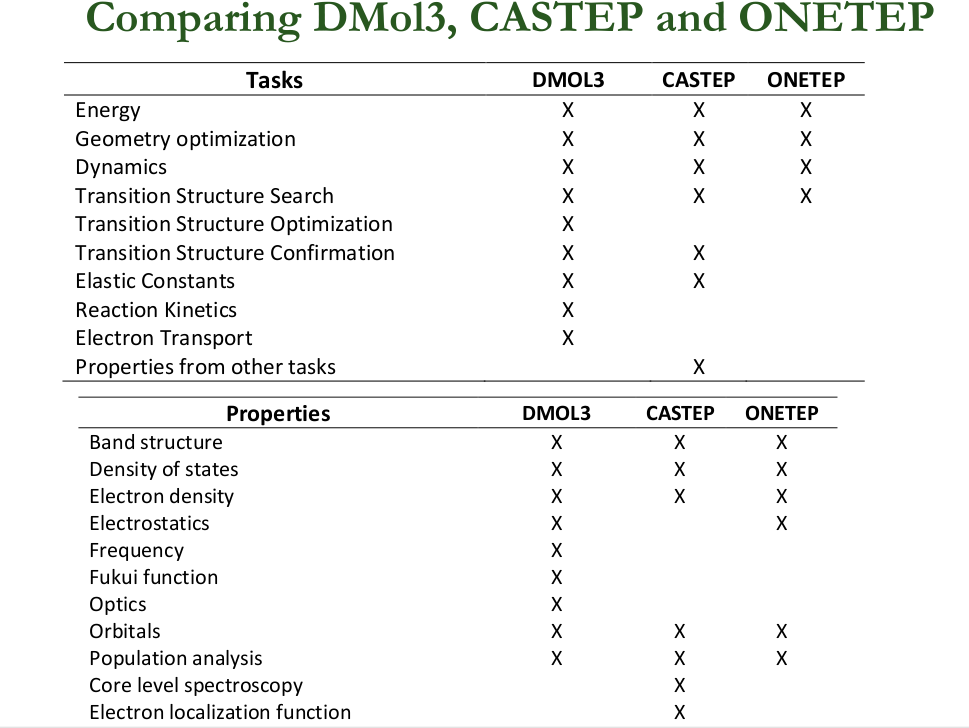
\includegraphics[height=2.70in,width=3.60in,viewport=0 0 969 728,clip]{Figures/MS-Caluculator-compare-2.png}
\caption{\tiny \textrm{Calculation modules comparison in Materials studio.}}%(与文献\cite{EPJB33-47_2003}图1对比)
\label{MS-Module_xc-functional}
\end{figure}
}

\frame
{
	\frametitle{\textrm{MS~Calculation:~ONETEP}}
\begin{figure}[h!]
\centering
\vspace*{-0.12in}
\includegraphics[height=2.15in,width=2.14in,viewport=0 0 646 650,clip]{Figures/MS-Caluculator_ONETEP-parameter.png}
\includegraphics[height=2.15in,width=1.68in,viewport=0 0 605 776,clip]{Figures/MS-Caluculator_ONETEP-analysis.png}
\caption{\tiny \textrm{Calculation module ONETEP in Materials studio.}}%(与文献\cite{EPJB33-47_2003}图1对比)
\label{MS-Calculation_ONETEP}
\end{figure}
}

\frame
{
	\frametitle{\textrm{MS~Calculation:~DFTB+ \& VAMP}}
\begin{figure}[h!]
\centering
\vspace*{-0.15in}
\includegraphics[height=2.00in,width=1.90in,viewport=0 0 635 671,clip]{Figures/MS-Caluculator_DFTB-parameter.png}
\includegraphics[height=2.00in,width=1.96in,viewport=0 0 723 739,clip]{Figures/MS-Caluculator_VAMP-parameter.png}
\caption{\tiny \textrm{Calculation parameters for module DFTB+ and VAMP in Materials studio.}}%(与文献\cite{EPJB33-47_2003}图1对比)
\label{MS-Calculation_DFTB-VAMP}
\end{figure}
}

\frame
{
	\frametitle{\textrm{MS~Calculation:~QMERA}}
\begin{figure}[h!]
\centering
\vspace*{-0.18in}
\includegraphics[height=2.58in,width=4.00in,viewport=0 0 1161 746,clip]{Figures/MS-Caluculator_QMERA-parameter.png}
\caption{\tiny \textrm{Calculation parameters for module QMERA in Materials studio.}}%(与文献\cite{EPJB33-47_2003}图1对比)
\label{MS-QMERA}
\end{figure}
}

\frame
{
	\frametitle{\textrm{Classical simulation:~Tools}}
\begin{figure}[h!]
\centering
\vspace*{-0.10in}
\includegraphics[height=1.91in,width=4.00in,viewport=0 0 1494 711,clip]{Figures/MS-Classical_simulation-tools.png}
\caption{\tiny \textrm{Calculation modules for classical simulation in Materials studio.}}%(与文献\cite{EPJB33-47_2003}图1对比)
\label{MS-Classical_simulation-}
\end{figure}
}

\frame
{
	\frametitle{\textrm{MS~Calculation:~Forcite Plus}}
\begin{figure}[h!]
\centering
\vspace*{-0.18in}
\includegraphics[height=2.70in,width=3.08in,viewport=0 0 845 741,clip]{Figures/MS-Caluculator_Forcite-parameter.png}
\caption{\tiny \textrm{Calculation modules Forcite in Materials studio.}}%(与文献\cite{EPJB33-47_2003}图1对比)
\label{MS-Forcite_Plus}
\end{figure}
}

\frame
{
	\frametitle{\textrm{MS~Calculation:~Adsorption Lactor}}
\begin{figure}[h!]
\centering
\vspace*{-0.18in}
\includegraphics[height=2.67in,width=4.00in,viewport=0 0 1093 728,clip]{Figures/MS-Caluculator_Adsorption-Lactor-example.png}
\caption{\tiny \textrm{Calculation modules Adsorption Lactor in Materials studio.}}%(与文献\cite{EPJB33-47_2003}图1对比)
\label{MS-Adsorption_Lactor}
\end{figure}
}

\frame
{
	\frametitle{\textrm{MS~Calculation:~Amorphous Cell}}
\begin{figure}[h!]
\centering
\vspace*{-0.18in}
\includegraphics[height=2.67in,width=2.53in,viewport=0 0 702 750,clip]{Figures/MS-Caluculator_Amorphous-Cell-parameter.png}
\caption{\tiny \textrm{Calculation modules Amorphous cell in Materials studio.}}%(与文献\cite{EPJB33-47_2003}图1对比)
\label{MS-Amorphous_cell}
\end{figure}
}

\frame
{
	\frametitle{\textrm{MS~Calculation:~Blends}}
\begin{figure}[h!]
\centering
\vspace*{-0.14in}
\includegraphics[height=2.43in,width=4.00in,viewport=0 0 1358 822,clip]{Figures/MS-Caluculator_Blends-example.png}
\caption{\tiny \textrm{Calculation modules Blends in Materials studio.}}%(与文献\cite{EPJB33-47_2003}图1对比)
\label{MS-Blends}
\end{figure}
}

\frame
{
	\frametitle{\textrm{MS~Calculation:~Conformers}}
\begin{figure}[h!]
\centering
\vspace*{-0.14in}
\includegraphics[height=2.33in,width=4.00in,viewport=0 0 1278 743,clip]{Figures/MS-Caluculator_Conformers-parameter.png}
\caption{\tiny \textrm{Calculation modules Conformers in Materials studio.}}%(与文献\cite{EPJB33-47_2003}图1对比)
\label{MS-Conformer}
\end{figure}
}

\frame
{
	\frametitle{\textrm{Mesoescale simulation:~Tools}}
\begin{figure}[h!]
\centering
%\vspace*{-0.10in}
\includegraphics[height=1.40in,width=4.00in,viewport=0 0 1391 482,clip]{Figures/MS-Mesoescale_simulation-tools.png}
\caption{\tiny \textrm{Calculation modules for mesoescale simulation in Materials studio.}}%(与文献\cite{EPJB33-47_2003}图1对比)
\label{MS-Mesoescale_simulation-}
\end{figure}
}

\frame
{
	\frametitle{\textrm{MS~Calculation:~Mesocite}}
\begin{figure}[h!]
\centering
%\vspace*{-0.14in}
\includegraphics[height=1.65in,width=4.00in,viewport=0 0 1188 488,clip]{Figures/MS-Caluculator_Mesocite-parameter.png}
\caption{\tiny \textrm{Calculation modules Mesocite in Materials studio.}}%(与文献\cite{EPJB33-47_2003}图1对比)
\label{MS-Mesocite}
\end{figure}
}

\frame
{
	\frametitle{\textrm{MS~Analytical and crystallization tools}}
\begin{figure}[h!]
\centering
\vspace*{-0.18in}
\includegraphics[height=2.70in,width=2.61in,viewport=0 0 850 821,clip]{Figures/MS-Analysis-cry_tools.png}
\caption{\tiny \textrm{Analytical and crystallization tools in Materials studio.}}%(与文献\cite{EPJB33-47_2003}图1对比)
\label{MS-Analysis-cry}
\end{figure}
}

\frame
{
	\frametitle{\textrm{MS~Analysis:~Reflex}}
\begin{figure}[h!]
\centering
%\vspace*{-0.14in}
\includegraphics[height=1.36in,width=4.00in,viewport=0 0 1374 467,clip]{Figures/MS-Analysis_Reflex.png}
\caption{\tiny \textrm{Analysis module Reflex overview in Materials studio.}}%(与文献\cite{EPJB33-47_2003}图1对比)
\label{MS-Analysis-Reflex-overview}
\end{figure}
}

\frame
{
	\frametitle{\textrm{MS~Analysis:~Reflex}}
\begin{figure}[h!]
\centering
\vspace*{-0.14in}
\includegraphics[height=2.47in,width=4.00in,viewport=0 0 1256 775,clip]{Figures/MS-Analysis_Reflex-example.png}
\caption{\tiny \textrm{Reflex pattern processing in Materials studio.}}%(与文献\cite{EPJB33-47_2003}图1对比)
\label{MS-Analysis-Reflex-example-1}
\end{figure}
}

\frame
{
	\frametitle{\textrm{Reflex:~Pattern Processing}}
\begin{figure}[h!]
\centering
\vspace*{-0.10in}
\includegraphics[height=1.63in,width=4.00in,viewport=0 0 1349 548,clip]{Figures/MS-Analysis_Reflex_Pattern-Processing.png}
\caption{\tiny \textrm{Pattern Processing parameters in Materials studio.}}%(与文献\cite{EPJB33-47_2003}图1对比)
\label{Reflex-Pattern-Processing}
\end{figure}
}

\frame
{
	\frametitle{\textrm{MS~Analysis:~Reflex}}
\begin{figure}[h!]
\centering
\vspace*{-0.14in}
\includegraphics[height=2.41in,width=4.00in,viewport=0 0 1270 764,clip]{Figures/MS-Analysis_Reflex_Powder-Diffraction-example.png}
\caption{\tiny \textrm{Reflex powder diffraction in Materials studio.}}%(与文献\cite{EPJB33-47_2003}图1对比)
\label{MS-Analysis-Reflex-example-2}
\end{figure}
}

\frame
{
	\frametitle{\textrm{Reflex:~Powder Diffraction}}
\begin{figure}[h!]
\centering
\vspace*{-0.10in}
\includegraphics[height=1.92in,width=4.00in,viewport=0 0 1343 644,clip]{Figures/MS-Analysis_Reflex_Powder-Diffraction-1.png}
\caption{\tiny \textrm{Powder Diffraction parameters in Materials studio.}}%(与文献\cite{EPJB33-47_2003}图1对比)
\label{Reflex-Powder_Diffraction-1}
\end{figure}
}

\frame
{
	\frametitle{\textrm{Reflex:~Powder Diffraction}}
\begin{figure}[h!]
\centering
\vspace*{-0.10in}
\includegraphics[height=1.70in,width=4.00in,viewport=0 0 1342 569,clip]{Figures/MS-Analysis_Reflex_Powder-Diffraction-2.png}
\caption{\tiny \textrm{Powder Diffraction parameters in Materials studio.}}%(与文献\cite{EPJB33-47_2003}图1对比)
\label{Reflex-Powder_Diffraction-2}
\end{figure}
}

\frame
{
	\frametitle{\textrm{Reflex:~Powder Indexing}}
\begin{figure}[h!]
\centering
\vspace*{-0.10in}
\includegraphics[height=1.63in,width=4.00in,viewport=0 0 1349 548,clip]{Figures/MS-Analysis_Reflex_Powder-Indexing.png}
\caption{\tiny \textrm{Powder Indexing parameters in Materials studio.}}%(与文献\cite{EPJB33-47_2003}图1对比)
\label{Reflex-Powder-Indexing}
\end{figure}
}

\frame
{
	\frametitle{\textrm{Reflex:~Powder Refinement}}
\begin{figure}[h!]
\centering
\vspace*{-0.18in}
\includegraphics[height=2.70in,width=2.30in,viewport=0 0 620 732,clip]{Figures/MS-Analysis_Reflex_Powder-Refinement.png}
\caption{\tiny \textrm{Powder Refinement parameters in Materials studio.}}%(与文献\cite{EPJB33-47_2003}图1对比)
\label{Reflex-Powder-Refinement}
\end{figure}
}

\frame
{
	\frametitle{\textrm{Reflex:~Powder QPA}}
\begin{figure}[h!]
\centering
%\vspace*{-0.18in}
\includegraphics[height=1.92in,width=4.00in,viewport=0 0 1296 621,clip]{Figures/MS-Analysis_Reflex_Powder-QPA.png}
\caption{\tiny \textrm{Powder QPA parameters in Materials studio.}}%(与文献\cite{EPJB33-47_2003}图1对比)
\label{Reflex-Powder-QPA}
\end{figure}
}

\frame
{
	\frametitle{\textrm{MS~Analysis:~Morphology}}
\begin{figure}[h!]
\centering
\vspace*{-0.18in}
\includegraphics[height=2.70in,width=3.06in,viewport=0 0 817 722,clip]{Figures/MS-Crystallization-example.png}
\caption{\tiny \textrm{Example:~Morphology calculation in Materials studio.}}%(与文献\cite{EPJB33-47_2003}图1对比)
\label{MS-Morphology}
\end{figure}
}

\appendix
\section{附录:~\rm{Linux}命令简介}
\frame
{
	\frametitle{与目录和文件有关的命令}
	\begin{itemize}
\setlength{\itemsep}{-10pt}
		\item \textcolor{blue}{mkdir}:~创建目录
\begin{figure}[h!]
\centering
\vspace{-11.5pt}
\includegraphics[height=1.2in,width=3.9in,viewport=0 220 800 470,clip]{Figures/Ubuntu-mkdir.png}
%\caption{\textrm{The wave-particle duality and Photoelectric effect}}
\label{Linux-command-mkdir}
\end{figure}
		\item \textcolor{blue}{cd}:~改变工作目录
\begin{figure}[h!]
\centering
\vspace{-9.5pt}
\includegraphics[height=0.8in,width=3.9in,viewport=0 310 800 470,clip]{Figures/Ubuntu-cd.png}
%\caption{\textrm{The wave-particle duality and Photoelectric effect}}
\label{Linux-command-cd}
\end{figure}
	\end{itemize}
}

\frame
{
	\frametitle{与目录和文件有关的命令}
	\begin{itemize}
		\item \textcolor{blue}{chmod}:~改变工作目录的权限
\begin{figure}[h!]
\centering
\vspace{-9.5pt}
\includegraphics[height=2.3in,width=3.9in,viewport=0 0 800 470,clip]{Figures/Ubuntu-chmod.png}
%\caption{\textrm{The wave-particle duality and Photoelectric effect}}
\label{Linux-command-chmod}
\end{figure}
	\end{itemize}
}

\frame
{
	\frametitle{与目录和文件有关的命令}
	\begin{itemize}
		\item \textcolor{blue}{chown}:~改变文件的属主
\begin{figure}[h!]
\centering
\vspace{-2.5pt}
\includegraphics[height=2.1in,width=3.9in,viewport=0 70 800 470,clip]{Figures/Ubuntu-chown.png}
%\caption{\textrm{The wave-particle duality and Photoelectric effect}}
\label{Linux-command-chown}
\end{figure}
	\end{itemize}
}

\frame
{
	\frametitle{与目录和文件有关的命令}
	\begin{itemize}
		\item \textcolor{blue}{cp}:~将文件\textrm{copy}到另一个文件或另一目录
\begin{figure}[h!]
\centering
\vspace{-2.5pt}
\includegraphics[height=2.2in,width=3.9in,viewport=0 0 800 470,clip]{Figures/Ubuntu-cp.png}
%\caption{\textrm{The wave-particle duality and Photoelectric effect}}
\label{Linux-command-cp}
\end{figure}
	\end{itemize}
}

\frame
{
	\frametitle{与目录和文件有关的命令}
	\begin{itemize}
\setlength{\itemsep}{-10pt}
		\item \textcolor{blue}{diff}:~逐行比较两个文件,列出不同
\begin{figure}[h!]
\centering
\vspace{-11.5pt}
\includegraphics[height=1.0in,width=3.9in,viewport=0 250 800 470,clip]{Figures/Ubuntu-diff.png}
%\caption{\textrm{The wave-particle duality and Photoelectric effect}}
\label{Linux-command-diff}
\end{figure}
		\item \textcolor{blue}{find}:~搜索文件\textrm{(\textcolor{magenta}{文件所在位置检索})}
\begin{figure}[h!]
\centering
\vspace{-11.5pt}
\includegraphics[height=1.0in,width=3.9in,viewport=0 270 800 470,clip]{Figures/Ubuntu-find.png}
%\caption{\textrm{The wave-particle duality and Photoelectric effect}}
\label{Linux-command-find}
\end{figure}
\end{itemize}
}

\frame
{
	\frametitle{与目录和文件有关的命令}
	\begin{itemize}
\setlength{\itemsep}{-10pt}
		\item \textcolor{blue}{grep}:~按给定模式搜索文件\textrm{(\textcolor{magenta}{文件所含内容搜索})}
\begin{figure}[h!]
\centering
\vspace{-12.5pt}
\includegraphics[height=1.0in,width=3.9in,viewport=0 250 800 470,clip]{Figures/Ubuntu-grep.png}
%\caption{\textrm{The wave-particle duality and Photoelectric effect}}
\label{Linux-command-grep}
\end{figure}
		\item \textcolor{blue}{head}:~显示指定文件前若干行
\begin{figure}[h!]
\centering
\vspace{-12.5pt}
\includegraphics[height=1.2in,width=3.9in,viewport=0 200 800 470,clip]{Figures/Ubuntu-head.png}
%\caption{\textrm{The wave-particle duality and Photoelectric effect}}
\label{Linux-command-head}
\end{figure}
\end{itemize}
}

\frame
{
	\frametitle{与目录和文件有关的命令}
	\begin{itemize}
		\item \textcolor{blue}{ln}:~建立文件链接\textrm{(link)}
\begin{figure}[h!]
\centering
\vspace{-18.5pt}
\includegraphics[height=2.0in,width=3.8in,viewport=0 50 800 470,clip]{Figures/Ubuntu-ln.png}
%\caption{\textrm{The wave-particle duality and Photoelectric effect}}
\label{Linux-command-ln}
\end{figure}
\vspace{-18.5pt}
\textcolor{red}{注意1:}~\textcolor{blue}{cp~-r}~会将链接文件\textrm{copy}成独立文件,如果需要保护文件符号链接\textrm{(软链接)}属性,建议用\textcolor{blue}{tar}命令\\
\textcolor{red}{注意2:}~不在同一文件系统\textrm{(如位于不同磁盘分区)}中的文件只能用符号链接,不能用硬链接
	\end{itemize}
}

\frame
{
	\frametitle{与目录和文件有关的命令}
	\begin{itemize}
		\item \textcolor{blue}{ls}:~列出目录中的内容
\begin{figure}[h!]
\centering
\vspace{-2.5pt}
\includegraphics[height=2.2in,width=3.9in,viewport=0 0 800 470,clip]{Figures/Ubuntu-ls.png}
%\caption{\textrm{The wave-particle duality and Photoelectric effect}}
\label{Linux-command-ls}
\end{figure}
	\end{itemize}
}

\frame
{
	\frametitle{与目录和文件有关的命令}
\begin{minipage}{0.58\textwidth}
\begin{itemize}
	\item \textcolor{blue}{more:}~分屏显示信息
\begin{figure}[h!]
\centering
\hspace*{-32.5pt}
\vspace{-18.5pt}
\includegraphics[height=1.8in,width=2.7in,viewport=0 0 800 500,clip]{Figures/Ubuntu-more.png}
%\caption{\textrm{The wave-particle duality and Photoelectric effect}}
\label{Linux-command-more}
\end{figure}
	\end{itemize}
\end{minipage}
\begin{minipage}{0.38\textwidth}
	\begin{itemize}
		\item \textcolor{brown}{-c}~清屏而非滚屏
		\item \textcolor{brown}{-f}~遇长行不折回
		\item \textrm{i}空格~显示后续\textrm{i}行
		\item \textrm{q}或\textrm{Q}~退出\textcolor{blue}{more}
		\item \textrm{=}~显示当前行号
		\item \textrm{h}~帮助信息
	\end{itemize}
\end{minipage}
}

\frame
{
	\frametitle{与目录和文件有关的命令}
	\begin{itemize}
		\item \textcolor{blue}{mv}:~文件或目录的移动或更名
\begin{figure}[h!]
\centering
\vspace{-12.5pt}
\includegraphics[height=2.3in,width=3.9in,viewport=0 0 800 550,clip]{Figures/Ubuntu-mv.png}
%\caption{\textrm{The wave-particle duality and Photoelectric effect}}
\label{Linux-command-mv}
\end{figure}
	\end{itemize}
}

\frame
{
	\frametitle{与目录和文件有关的命令}
	\begin{itemize}
\setlength{\itemsep}{-10pt}
		\item \textcolor{blue}{pwd}:~显示当前目录绝对路径
\begin{figure}[h!]
\centering
\vspace{-15.5pt}
\includegraphics[height=0.6in,width=3.9in,viewport=0 0 800 160,clip]{Figures/Ubuntu-pwd.png}
%\caption{\textrm{The wave-particle duality and Photoelectric effect}}
\label{Linux-command-pwd}
\end{figure}
		\item \textcolor{blue}{rm}:~删除文件或目录
\begin{figure}[h!]
\centering
\vspace{-15.5pt}
\includegraphics[height=1.7in,width=3.9in,viewport=0 120 800 550,clip]{Figures/Ubuntu-rm.png}
%\caption{\textrm{The wave-particle duality and Photoelectric effect}}
\label{Linux-command-rm}
\end{figure}
\end{itemize}
}

\frame
{
	\frametitle{与目录和文件有关的命令}
\begin{minipage}{0.48\textwidth}
\begin{itemize}
	\item \textcolor{blue}{sort:}~对指定文件按行排序
\begin{figure}[h!]
\centering
\hspace*{-28.5pt}
\vspace{18.5pt}
\includegraphics[height=1.3in,width=2.1in,viewport=0 350 400 600,clip]{Figures/Ubuntu-sort.png}
%\caption{\textrm{The wave-particle duality and Photoelectric effect}}
\label{Linux-command-sort}
\end{figure}
	\end{itemize}
\end{minipage}
\begin{minipage}{0.50\textwidth}
	\begin{itemize}
		\item \textcolor{brown}{-b}~忽略开头的空格和制表符
		\item \textcolor{brown}{-d}~仅字母、数字、空格按字典排序
		\item \textcolor{brown}{-f}~不区分字母大小写
		\item \textcolor{brown}{-n}~按数字升序排列
		\item \textcolor{brown}{-r}~按当前顺序的逆序排序
		\item \textcolor{brown}{-u}~忽略重复行
		\item \textcolor{brown}{-o}~指定输出文件名
	\end{itemize}
\end{minipage}
}

\frame
{
	\frametitle{与目录和文件有关的命令}
	\begin{itemize}
		\item \textcolor{blue}{tail}:~显示指定文件的最后部分
\begin{figure}[h!]
\centering
\vspace{-12.5pt}
\includegraphics[height=2.3in,width=3.9in,viewport=0 0 800 480,clip]{Figures/Ubuntu-tail.png}
%\caption{\textrm{The wave-particle duality and Photoelectric effect}}
\label{Linux-command-tail}
\end{figure}
	\end{itemize}
}

\frame
{
	\frametitle{与目录和文件有关的命令}
	\begin{itemize}
		\item \textcolor{blue}{tar}:~将若干文件存档或读取存档文件
\begin{figure}[h!]
\centering
\vspace{-12.5pt}
\includegraphics[height=2.3in,width=3.9in,viewport=0 10 800 530,clip]{Figures/Ubuntu-tar.png}
%\caption{\textrm{The wave-particle duality and Photoelectric effect}}
\label{Linux-command-tar}
\end{figure}
	\end{itemize}
}

\frame
{
	\frametitle{与目录和文件有关的命令}
	\begin{itemize}
		\item \textcolor{blue}{wc}:~统计指定文件的行数、词数和字符数
\begin{figure}[h!]
\centering
\vspace{-12.5pt}
\includegraphics[height=2.3in,width=3.9in,viewport=0 60 800 560,clip]{Figures/Ubuntu-wc.png}
%\caption{\textrm{The wave-particle duality and Photoelectric effect}}
\label{Linux-command-wc}
\end{figure}
	\end{itemize}
}

\frame
{
	\frametitle{状态信息查询命令}
	\begin{itemize}
\setlength{\itemsep}{-10pt}
		\item \textcolor{blue}{date}:~显示日期与时间
\begin{figure}[h!]
\centering
\vspace{-15.5pt}
\includegraphics[height=0.6in,width=3.9in,viewport=0 0 800 130,clip]{Figures/Ubuntu-date.png}
%\caption{\textrm{The wave-particle duality and Photoelectric effect}}
\label{Linux-command-date}
\end{figure}
		\item \textcolor{blue}{df}:~查询磁盘空间使用情况
\begin{figure}[h!]
\centering
\vspace{-15.5pt}
\includegraphics[height=1.7in,width=3.9in,viewport=0 150 800 530,clip]{Figures/Ubuntu-df.png}
%\caption{\textrm{The wave-particle duality and Photoelectric effect}}
\label{Linux-command-df}
\end{figure}
\end{itemize}
}

\frame
{
	\frametitle{状态信息查询命令}
	\begin{itemize}
		\item \textcolor{blue}{du}:~统计目录或文件所占磁盘空间的大小
\begin{figure}[h!]
\centering
\vspace{-5.5pt}
\includegraphics[height=2.1in,width=3.6in,viewport=0 0 800 580,clip]{Figures/Ubuntu-du-1.png}
\includegraphics[height=0.6in,width=3.7in,viewport=0 0 880 150,clip]{Figures/Ubuntu-du-2.png}
%\caption{\textrm{The wave-particle duality and Photoelectric effect}}
\label{Linux-command-du}
\end{figure}
	\end{itemize}
}

\frame
{
	\frametitle{状态信息查询命令}
	\begin{itemize}
\setlength{\itemsep}{-15pt}
		\item \textcolor{blue}{ps}:~检查进程状态
\begin{figure}[h!]
\centering
\vspace{-10.5pt}
\includegraphics[height=0.9in,width=3.7in,viewport=0 20 850 230,clip]{Figures/Ubuntu-ps.png}
%\caption{\textrm{The wave-particle duality and Photoelectric effect}}
\label{Linux-command-ps}
\end{figure}
		\item \textcolor{blue}{time}:~统计程序或命令运行的时间
\begin{figure}[h!]
\centering
\vspace{-5.5pt}
\includegraphics[height=0.7in,width=3.7in,viewport=0 20 850 180,clip]{Figures/Ubuntu-time.png}
%\caption{\textrm{The wave-particle duality and Photoelectric effect}}
\label{Linux-command-time}
\end{figure}
		\item \textcolor{blue}{w}:~检查状态状态
\begin{figure}[h!]
\centering
\vspace{-18.5pt}
\includegraphics[height=0.7in,width=3.8in,viewport=0 0 850 150,clip]{Figures/Ubuntu-w.png}
%\caption{\textrm{The wave-particle duality and Photoelectric effect}}
\label{Linux-command-w}
\end{figure}
\end{itemize}
}

\frame
{
	\frametitle{状态信息查询命令}
	\begin{itemize}
		\item \textcolor{blue}{whereis}:~确定命令位置
		\item \textcolor{blue}{which}:~确定命令位置
		\item \textcolor{blue}{who}:~列出正在使用系统的用户
		\item \textcolor{blue}{whoami}:~显示正在使用本终端的用户名
	\end{itemize}
\begin{figure}[h!]
\centering
\vspace{-5.5pt}
\includegraphics[height=1.4in,width=3.9in,viewport=0 30 800 300,clip]{Figures/Ubuntu-which.png}
%\caption{\textrm{The wave-particle duality and Photoelectric effect}}
\label{Linux-command-which}
\end{figure}
}

\frame
{
	\frametitle{网络查询命令}
	\begin{itemize}
		\item \textcolor{blue}{arp}:~网络和\textrm{IP}地址查询
		\item \textcolor{blue}{ifconfig}:~网络和\textrm{MAC}地址查询
	\end{itemize}
\begin{figure}[h!]
\centering
\vspace{-5.5pt}
\includegraphics[height=2.1in,width=3.9in,viewport=0 0 800 470,clip]{Figures/Ubuntu-netip.png}
%\caption{\textrm{The wave-particle duality and Photoelectric effect}}
\label{Linux-command-netip}
\end{figure}
}

\frame
{
	\frametitle{远程登录命令}
	\begin{itemize}
		\item \textcolor{blue}{ssh}:~远程登录
\begin{figure}[h!]
\centering
\vspace{-10.5pt}
\includegraphics[height=2.4in,width=3.9in,viewport=0 0 800 550,clip]{Figures/Ubuntu-ssh.png}
%\caption{\textrm{The wave-particle duality and Photoelectric effect}}
\label{Linux-command-ssh}
\end{figure}
	\end{itemize}
}

\frame
{
	\frametitle{远程无密码登录}
\begin{figure}[h!]
\centering
\vspace{-13.2pt}
\includegraphics[height=3.02in,width=2.9in,viewport=0 0 1080 1130,clip]{Figures/Ubuntu-auto-ssh.png}
%\caption{\textrm{The wave-particle duality and Photoelectric effect}}
\label{Linux-command-auto-ssh}
\end{figure}
}

\frame
{
	\frametitle{远程传输命令}
	\begin{itemize}
		\item \textcolor{blue}{scp}:~远程传输
\begin{figure}[h!]
\centering
\vspace{-10.5pt}
\includegraphics[height=0.65in,width=3.9in,viewport=0 0 1080 200,clip]{Figures/Ubuntu-scp.png}
%\caption{\textrm{The wave-particle duality and Photoelectric effect}}
\label{Linux-command-scp}
\end{figure}
	\end{itemize}
}

\frame
{
	\frametitle{程序运行命令}
	\begin{itemize}
\setlength{\itemsep}{-10pt}
		\item \textcolor{blue}{echo}:~参数回应至标准输出
\begin{figure}[h!]
\centering
\vspace{-15.5pt}
\includegraphics[height=1.1in,width=3.9in,viewport=0 0 800 230,clip]{Figures/Ubuntu-echo.png}
%\caption{\textrm{The wave-particle duality and Photoelectric effect}}
\label{Linux-command-echo}
\end{figure}
		\item \textcolor{blue}{kill}:~终止指定进程
\begin{figure}[h!]
\centering
\vspace{-15.5pt}
\includegraphics[height=0.8in,width=3.9in,viewport=0 0 800 180,clip]{Figures/Ubuntu-kill.png}
%\caption{\textrm{The wave-particle duality and Photoelectric effect}}
\label{Linux-command-kill}
\end{figure}
\end{itemize}
}

\frame
{
	\frametitle{程序运行命令}
	\begin{itemize}
		\item \textcolor{blue}{tee}:~将标准输出同时复制到文件
\begin{figure}[h!]
\centering
\vspace{-10.5pt}
\includegraphics[height=1.15in,width=3.9in,viewport=0 0 800 260,clip]{Figures/Ubuntu-tee.png}
%\caption{\textrm{The wave-particle duality and Photoelectric effect}}
\label{Linux-command-tee}
\end{figure}
	\end{itemize}
}

\frame
{
	\frametitle{其它命令}
	\begin{itemize}
\setlength{\itemsep}{-5pt}
		\item \textcolor{blue}{cal}:~打印日历
\begin{figure}[h!]
\centering
\vspace{-5.5pt}
\includegraphics[height=1.7in,width=3.4in,viewport=0 110 700 480,clip]{Figures/Ubuntu-cal.png}
%\caption{\textrm{The wave-particle duality and Photoelectric effect}}
\label{Linux-command-cal}
\end{figure}
		\item \textcolor{blue}{passwd}:~变更当前账户的密码
\begin{figure}[h!]
\centering
\vspace{-5.5pt}
\includegraphics[height=0.55in,width=3.4in,viewport=0 0 700 120,clip]{Figures/Ubuntu-passwd.png}
%\caption{\textrm{The wave-particle duality and Photoelectric effect}}
\label{Linux-command-passwd}
\end{figure}
\end{itemize}
}

\frame
{
	\frametitle{其它命令}
	\begin{itemize}
		\item \textcolor{blue}{man}:~查询参考手册信息
	\end{itemize}
\begin{figure}[h!]
\centering
\vspace{-7.5pt}
\includegraphics[height=2.65in,width=4.0in,viewport=0 0 1410 860,clip]{Figures/Ubuntu-man.png}
%\caption{\textrm{The wave-particle duality and Photoelectric effect}}
\label{Linux-command-man}
\end{figure}
}

\frame
{
	\frametitle{\textrm{Ubuntu}下的软件安装与系统更新}
\begin{figure}[h!]
\centering
\vspace{-11.5pt}
\includegraphics[height=0.74\textwidth]{Figures/Ubuntu-apt-get.png}
%\caption{\fontsize{6.2pt}{5.2pt}\selectfont{欧阳修(1007-1072)~《欧阳文忠公文集$\cdot$归田录》~卷上}}
\label{Ubuntu-apt-get}
\end{figure}
}

\frame
{
	\frametitle{卖油翁:~\textcolor{red}{无他~但手熟尔}}
%陈康肃公尧咨善射,当世无双 ,公亦以此自矜。尝射于家圃,有卖油翁释担而立,睨之,久而不去。见其发矢十中八、九,但微颔之。康肃问曰:“汝亦知射乎?吾射不亦精乎?”翁曰:“无他,但手熟尔。”康肃忿然曰:“尔安敢轻吾射!”翁曰:“以我酌油知之。”乃取一葫芦置于地,以钱覆其口,徐以杓酌油沥之,自钱孔入而\footnote{一作“而入”}钱不湿。因曰:“\textcolor{red}{我亦无他,惟手熟尔}。”康肃笑而遣之。此与庄生所谓“解牛”、“斫轮”者何异?
\begin{figure}[h!]
\centering
\vspace{-10.5pt}
\includegraphics[height=0.65\textwidth]{Figures/Sale_Oil_Ouyang.png}
\hspace{1pt}
\includegraphics[height=0.65\textwidth]{Figures/Ouyang_Xiu-2.jpg}
\caption{\fontsize{6.2pt}{5.2pt}\selectfont{欧阳修(1007-1072)~《欧阳文忠公文集$\cdot$归田录》~卷上}}
\label{Sale_oil}
\end{figure}
}

